\documentclass[11pt,a4paper]{article}

% Preamble: packages, theorem environments, and page furniture.

\usepackage[T1]{fontenc}
\usepackage{lmodern}
\usepackage{microtype}

\usepackage[a4paper,margin=27mm]{geometry}
\usepackage{ragged2e}
\usepackage{amsmath}
\usepackage{amssymb}
\usepackage{amsthm}
\usepackage{booktabs}
\usepackage{longtable}
\usepackage{array}
\usepackage{enumitem}
\usepackage{verbatim}
\usepackage{xcolor}
\usepackage{fancyvrb}
\usepackage{tikz}
\usetikzlibrary{arrows.meta,positioning}

% Identifiers and paths set in \texttt are the only things in this document
% long enough to overflow a line; htt lets TeX hyphenate them, and the
% emergency stretch absorbs what is left.
\usepackage[htt]{hyphenat}
\setlength{\emergencystretch}{2.5em}

\usepackage[hidelinks]{hyperref}
\usepackage[capitalise,noabbrev]{cleveref}

% One shared counter for every numbered result, so a reference to "Theorem 12"
% can never collide with "Lemma 12" and the reader can find any of them by
% counting forwards.
\theoremstyle{plain}
\newtheorem{theorem}{Theorem}
\newtheorem{lemma}[theorem]{Lemma}
\newtheorem{proposition}[theorem]{Proposition}
\newtheorem{corollary}[theorem]{Corollary}

\theoremstyle{definition}
\newtheorem{definition}[theorem]{Definition}
\newtheorem{example}[theorem]{Example}
\newtheorem{obligation}[theorem]{Proof obligation}

\theoremstyle{remark}
\newtheorem{remark}[theorem]{Remark}

\crefname{obligation}{proof obligation}{proof obligations}
\Crefname{obligation}{Proof obligation}{Proof obligations}

% Pseudocode transcribed from the specification. Kept verbatim rather than
% reset in a pretty algorithm environment: the whole point is that the reader
% can diff it against SPEC.md by eye.
\DefineVerbatimEnvironment{speccode}{Verbatim}%
  {fontsize=\small,frame=leftline,framerule=0.6pt,%
   xleftmargin=10pt,framesep=8pt}

% Table columns hold package names, test identifiers and other unbreakable
% strings; ragged right is the only setting under which they do not overflow.
\newcolumntype{L}[1]{>{\RaggedRight\arraybackslash}p{#1}}

\setlist{itemsep=2pt,topsep=4pt,parsep=0pt}
\setlength{\parskip}{0.4em}
\setlength{\parindent}{0pt}

\hypersetup{
  pdftitle={The CCME release guarantees: a formal model and proofs},
  pdfsubject={Formal properties of the Conventional Commits Monorepo Extension release algorithm},
  pdfkeywords={release engineering, monorepo, semantic versioning, convergence, distributed transactions}
}

% One macro per notion of the specification. Nothing in this document types a
% symbol directly: if a definition changes, it changes here, and the appendix
% symbol table is written from this file.

% ---- cross-references into the sources -------------------------------------
% \textup so that small caps survive the italic body of a theorem environment,
% where T1/lmr/m/scit does not exist.
\newcommand{\SPEC}{\textup{\textsc{spec}}}
\newcommand{\spec}[1]{\SPEC~\S#1}
\newcommand{\specs}[2]{\SPEC~\S\S#1,~#2}
\newcommand{\code}[1]{\texttt{#1}}
\newcommand{\diag}[1]{\texttt{#1}}          % a diagnostic code, e.g. \diag{W208}

% ---- history ---------------------------------------------------------------
\newcommand{\Cmts}{\ensuremath{\mathcal{K}}}            % the set of commits
\newcommand{\Head}{\ensuremath{h}}                      % HEAD, fixed throughout
\newcommand{\Rch}[1]{\ensuremath{\mathrm{reach}(#1)}}   % ancestors-or-self
\newcommand{\anc}{\ensuremath{\preceq}}                 % ancestor-or-self

% ---- workspace -------------------------------------------------------------
\newcommand{\Pkgs}{\ensuremath{\mathcal{P}}}            % packages at HEAD
\newcommand{\Edges}{\ensuremath{E}}                     % dependency edges
\newcommand{\Dep}[1]{\ensuremath{\mathrm{dep}(#1)}}     % direct dependents of a package
\newcommand{\dist}[2]{\ensuremath{\delta(#1,#2)}}       % shortest edge count, set to package
\newcommand{\reachset}[2]{\ensuremath{R(#1,#2)}}        % the traversal of §9.2

% ---- bumps and versions ----------------------------------------------------
\newcommand{\Bumps}{\ensuremath{\mathbb{B}}}
\newcommand{\bnone}{\ensuremath{\mathsf{none}}}
\newcommand{\bpatch}{\ensuremath{\mathsf{patch}}}
\newcommand{\bminor}{\ensuremath{\mathsf{minor}}}
\newcommand{\bmajor}{\ensuremath{\mathsf{major}}}
\newcommand{\Vers}{\ensuremath{\mathcal{V}}}
\newcommand{\applyb}[2]{\ensuremath{\mathrm{apply}(#1,#2)}}
\newcommand{\coreof}[1]{\ensuremath{\mathrm{core}(#1)}}
\newcommand{\cntof}[1]{\ensuremath{\mathrm{cnt}(#1)}}

% ---- channels --------------------------------------------------------------
\newcommand{\Chans}{\ensuremath{\mathcal{C}\!h}}
\newcommand{\stable}{\ensuremath{\mathsf{stable}}}
\newcommand{\chanof}[1]{\ensuremath{\mathrm{ch}(#1)}}   % the channel of a version
\newcommand{\NONE}{\ensuremath{\bot}}                   % "proposes nothing"

% ---- state and its derived quantities --------------------------------------
\newcommand{\st}{\ensuremath{\sigma}}
\newcommand{\Win}[2]{\ensuremath{W_{#1}(#2)}}                  % train window
\newcommand{\Winf}[2]{\ensuremath{W^{\circ}_{#1}(#2)}}         % undelivered admission window
\newcommand{\base}[2]{\ensuremath{\mathrm{base}_{#1}(#2)}}
\newcommand{\basec}[2]{\ensuremath{\mathrm{basec}_{#1}(#2)}}   % commit of the baseline tag
\newcommand{\stbase}[2]{\ensuremath{\mathrm{sbase}_{#1}(#2)}}
\newcommand{\stcommit}[2]{\ensuremath{\mathrm{scom}_{#1}(#2)}}
\newcommand{\chanres}[2]{\ensuremath{\mathrm{chan}_{#1}(#2)}}  % channel(P), §13.8

% ---- units and their directives --------------------------------------------
\newcommand{\Units}{\ensuremath{\mathcal{U}}}
\newcommand{\cof}[1]{\ensuremath{c_{#1}}}                      % the commit carrying a unit
\newcommand{\scopef}[1]{\ensuremath{\mathrm{scope}(#1)}}
\newcommand{\bumpof}[1]{\ensuremath{\mathrm{bump}(#1)}}
\newcommand{\pbump}[1]{\ensuremath{\mathrm{pb}(#1)}}           % effective propagated bump
\newcommand{\pdepth}[1]{\ensuremath{\mathrm{pd}(#1)}}
\newcommand{\pscope}[1]{\ensuremath{\mathrm{ps}(#1)}}
\newcommand{\pchan}[1]{\ensuremath{\mathrm{pc}(#1)}}
\newcommand{\pcdepth}[1]{\ensuremath{\mathrm{pcd}(#1)}}
\newcommand{\pcscope}[1]{\ensuremath{\mathrm{pcs}(#1)}}

% ---- suppression, sources, admission ---------------------------------------
\newcommand{\disch}[3]{\ensuremath{\mathrm{disch}_{#1}(#2,#3)}}
\newcommand{\canc}[2]{\ensuremath{\mathrm{canc}(#1,#2)}}
\newcommand{\held}[1]{\ensuremath{\mathrm{held}(#1)}}
\newcommand{\srcp}[2]{\ensuremath{\mathrm{src}_{#1}(#2)}}
\newcommand{\srcch}[2]{\ensuremath{\mathrm{sch}_{#1}(#2)}}     % the source channel set, §9.3a
\newcommand{\resolv}[3]{\ensuremath{\mathrm{rsv}_{#1}(#2,#3)}}
\newcommand{\admit}[3]{\ensuremath{\mathrm{adm}_{#1}(#2,#3)}}

% ---- the plan --------------------------------------------------------------
\newcommand{\dirb}[2]{\ensuremath{\mathrm{dir}_{#1}(#2)}}
\newcommand{\propb}[2]{\ensuremath{\mathrm{prp}_{#1}(#2)}}
\newcommand{\effb}[2]{\ensuremath{\mathrm{eff}_{#1}(#2)}}
\newcommand{\plan}[1]{\ensuremath{\Pi(#1)}}
\newcommand{\vers}[2]{\ensuremath{\nu_{#1}(#2)}}
\newcommand{\Run}[2]{\ensuremath{\mathrm{run}(#1,#2)}}

% ---- guarantee labels ------------------------------------------------------
\newcommand{\G}[1]{\textbf{G#1}}

% ---- delivery (SPEC 13.3, 13.4a, 19.3; added for the 3.1.0-rc.2 text) ------
\newcommand{\relc}[2]{\ensuremath{T_{#1}(#2)}}                        % release commits of a package
\newcommand{\deliv}[4]{\ensuremath{\mathrm{dlv}_{#1}(#2,#3,#4)}}       % delivered(P, C, D)
\newcommand{\owed}[3]{\ensuremath{\mathrm{owed}_{#1}(#2,#3)}}          % owed(u, D)
\newcommand{\Wowed}[3]{\ensuremath{W^{\mathrm{ow}}_{#1}(#2,#3)}}       % owedWindow(P, D)
\newcommand{\owes}[3]{\ensuremath{\mathrm{owes}_{#1}(#2,#3)}}          % P still owes D
\newcommand{\owncause}[3]{\ensuremath{\mathrm{own}_{#1}(#2,#3)}}       % a cause of its own, §19.3
\newcommand{\wf}[1]{\ensuremath{\mathrm{wf}(#1)}}                      % E201 well-formedness of a state
\newcommand{\pubset}[2]{\ensuremath{S(#1,#2)}}                         % the packages a run publishes
\newcommand{\blocked}[2]{\ensuremath{B(#1,#2)}}                        % the packages a run blocks
\newcommand{\stale}[2]{\ensuremath{\mathrm{stale}_{#1}(#2)}}           % the upward audit, §13.7b
\newcommand{\Kprop}{\ensuremath{K_{\mathrm{prop}}}}                    % propagation.kinds
\newcommand{\Korder}{\ensuremath{K_{\mathrm{order}}}}                  % publish.orderKinds
\newcommand{\Kblock}{\ensuremath{K_{\mathrm{block}}}}                  % publish.blockingKinds

% ---- execution section (moved from sections/04a-execution.tex) --------------
% Symbols of the execution section, prefixed \ex.
\newcommand{\exafter}[2]{\ensuremath{A_{#1}(#2)}}          % after-set in repository #1 of boundary #2
\newcommand{\exRch}[2]{\ensuremath{\mathrm{reach}_{#1}(#2)}} % reachability inside one repository
\newcommand{\exWin}[2]{\ensuremath{W(#1;\,#2)}}             % train window of consumer #1 over repository #2
\newcommand{\exWinf}[2]{\ensuremath{W^{\circ}(#1;\,#2)}}    % fresh window of consumer #1 over repository #2
\newcommand{\exPlan}{\ensuremath{\mathrm{Plan}}}            % the pure planning function of §28.3
\newcommand{\exI}{\ensuremath{\mathcal{I}}}                 % the fixed run input of §28.3
\newcommand{\exbuild}[1]{\ensuremath{\mathrm{build}(#1)}}
\newcommand{\expub}[1]{\ensuremath{\mathrm{publish}(#1)}}

% ---- evaluation section (moved from sections/11-evaluation.tex) -------------
% \evpath sets a file path in monospace and lets it break after / . _ and -,
% through the url package that hyperref already loads. \evhash lets a hex
% digest break anywhere, since nothing in it is a word.
\DeclareUrlCommand\evpath{\urlstyle{tt}\def\UrlBreaks{\do\/\do\.\do\_\do\-\do\@\do\:}}
\newcommand{\evRQ}[1]{\textbf{RQ#1}}
\makeatletter
\newcommand{\evhash}[1]{\texttt{\ev@split#1\@nil}}
\def\ev@split#1#2\@nil{#1\ifx\relax#2\relax\expandafter\@gobble\else\expandafter\@firstofone\fi{\allowbreak\ev@split#2\@nil}}
\makeatother


\title{The CCME Release Guarantees\\[2mm]
       \large A formal model, with proofs, of the release computation, its publish
       protocol and its execution profile, with the executed campaigns (extended edition)}
\author{Semen Fediukovich}
\date{September 2026 \\[2mm]
      \normalsize Technical report accompanying \texttt{specs/ccme-spec/SPEC.md} 3.1.0-rc.2\\
      \normalsize at commit \texttt{252216ba} of \texttt{github.com/yohimik/dispat}}

\begin{document}
\maketitle

\begin{abstract}
Releasing interdependent packages is a distributed transaction without a
coordinator or rollback: each publish is an irreversible write to an
independent registry. CCME defines a resumable release algorithm and states
eight guarantees: termination, completeness, version stability, exactly-once
tag-ledger delivery, retry-invariant non-widening and convergence, channel
discharge and one-way axis independence.

This report formalises the algorithm of the 3.1.0 release candidate and proves
the guarantees under its explicit retry invariant. The candidate replaces the
window test of earlier versions by delivery: a propagated contribution stays
owed to a consumer until the source has released it and the consumer has
released after that, which closes the orphan a consumer reaches by getting
ahead of a failed provider, at the price of an owed window per dependency edge
and a refusal (\diag{E201}) where two releases on one commit could hide a debt.
The report also proves the determinism and idempotency requirements of
\spec{17.2}, the duality of \spec{13.7b}, and transcribes what the candidate
adds around the computation: records read under the release lock
(\spec{13.2}), the three-valued build readiness relation of \spec{19.2a} with
the run durations it leads to, the distributed execution profile of \spec{28}
with the placement invariance and list-scheduling bounds it admits, and the
repository-local windows of \spec{27}. The cost bounds of \specs{13.11}{20.7}
are restated for the current text, including the single marker pass over
history.

Two ledgers of obligations follow: the current departures of the reference
implementation from the candidate, and the six failure classes found in
CCME 1.0.0 with their minimal counterexamples, kept as provenance. A
conformance table maps every result to the specification's vectors and to the
integration test that stands behind it. The final section reports every
executed campaign with its pinned binary and environment, including the two
measurements of 22 September 2026 on which the execution profile rests: the
two kernel farm groups that met their public reference times with a second
node, twice each after one rejected candidate, and an LLVM matrix released
through two workers in less time than on one node, once per side, with a
reproduction kit whose binary rebuilds were verified byte for byte and whose
machine definitions were planned but not applied. A condensed edition built
from the same sources keeps the findings, the model, the proofs, the ledger
of departures and the results.
\end{abstract}

\paragraph{Specification snapshot.}
The normative subject is \texttt{specs/ccme-spec/SPEC.md} as committed at
\texttt{252216bab9bd4052ba181a2ceb47e21363b8eff3}, stamped 3.1.0-rc.2 and
pending release as 3.1.0-rc.3 together with dispat 1.11.0-rc.4; its
\texttt{DESIGN-HISTORY.md} entries of 21 and 22 September 2026 record what the
engine implements. Where the report says \emph{the current text} it means this
commit. The historical audit of \cref{sec:obligations-historical} concerns
CCME 1.0.0 at \texttt{713f1a0b}; the released CCME 2.0.0 at
\texttt{d3ce8ae6} is cited where a change since then matters.\par

\tableofcontents
\newpage

\section{Introduction}
\label{sec:intro}

\subsection{The problem}

A workspace is a repository holding many independently versioned packages that
depend on one another. Releasing it means choosing a new version for each
package that needs one, writing those versions into manifests, uploading
artefacts to registries, and recording what happened.

The recording is the hard part. Registries have no transactions. A publish is an
irreversible write to a service the release tool does not control, several
registries may be involved (npm, a container registry, a language-specific
index), and there is no coordinator that can commit or abort them as a unit. A
run that publishes seven packages is seven independent, individually fallible
writes; it may finish having done four of them.

CCME\footnote{\emph{Conventional Commits: Monorepo Extension}, version
3.1.0-rc.2 at commit \texttt{252216ba}, \code{specs/ccme-spec/SPEC.md} in the
\code{dispat} repository. Referred to throughout as \SPEC{}, cited by section
number.} answers this the way a saga does. There is no external state file, no
lock service beyond the release lock itself, and no registry polling. The
release plan is a pure function of the repository at a fixed commit; each
completed leg of the transaction is recorded by an annotated git tag written
immediately after that leg succeeds; and recovery is re-execution: run the
engine again and it recomputes the same transaction, skipping the legs already
recorded.

That design only works if re-execution is well behaved, and \spec{13.7c} states
the eight properties that say it is:

\begin{description}[leftmargin=3.2em,style=nextline,font=\normalfont\bfseries]
  \item[\G{1} termination] propagation halts, whatever the declared depth.
  \item[\G{2} completeness] a contribution admitted to a dependent survives in
    every later run until that dependent releases at or after a release of
    every owed source carrying it; there are no orphans, whether the provider
    failed or the consumer got ahead of it.
  \item[\G{3} version stability] a package released late is released at the
    version it was originally planned at.
  \item[\G{4} no double ledger delivery] a contribution does not survive its
    delivery in the tag ledger; a consumer that proceeded past a commit before
    its source released it is bumped once more when that release comes, and
    that is the delivery, not a second one. This says nothing unconditional
    about external effects.
  \item[\G{5} no blast-radius widening] under the retry invariant, later
    targets are a subset of the first run's.
  \item[\G{6} restricted convergence] under the retry invariant, repeated
    successful progress empties the initial plan within as many runs as it had
    publishable packages.
  \item[\G{7} channel discharge] a prerelease channel is proposed to a package
    only until it is released on it.
  \item[\G{8} one-way axis independence] suppressing a version bump does not
    suppress a channel change; resolved channels may suppress bumps.
\end{description}

\subsection{Why formalise them, and what changed}

The specification proves each property briefly, while the algorithm is spread
across prose and pseudocode. This report writes the algorithm down once,
formally (\cref{sec:model,sec:propagation,sec:protocol}), and proves the
guarantees inside that model (\cref{sec:guarantees}), along with the
determinism and idempotency obligations of \spec{17.2}
(\cref{sec:determinism}), the duality of \spec{13.7b}
(\cref{sec:duality}), and the cost bounds and optimisation-equivalence claims
of \specs{13.11}{20.7} (\cref{sec:complexity}).

Earlier editions of this report formalised CCME 2.0.0, whose contribution was
to state the cross-run retry invariant explicitly and to separate the train
window from the undelivered window. The current text keeps both and changes
the admission test of the bump axis: where 2.0.0 admitted a propagated
contribution while the unit's commit lay in the dependent's undelivered
window, the candidate admits it while some source of the unit has not
\emph{delivered} that commit to the dependent, that is, while the dependent has
not released at or after a release of that source carrying it (\spec{13.4a}).
The two tests agree for every dependent that has not released past the commit.
They differ for a dependent that released past it before its provider did,
which the candidate's own publish protocol now allows: a consumer with a cause
of its own proceeds past a failed provider (\spec{19.3}) instead of being
blocked. Under the old test such a consumer was never planned again once the
provider published, an orphan reached from the consumer's side. Delivery
closes it, and two further rules follow from it: a window per dependency edge
that keeps the debt visible once the provider has released (\spec{13.3}), and a
refusal, \diag{E201}, where a provider would release at the very commit a
consumer it still owes was released at, because two releases on one commit
cannot be ordered afterwards. \Cref{sec:model,sec:propagation,sec:guarantees}
transcribe and prove the candidate's form; \cref{ob:samecommit} states the one
place where the ledger reports a loss instead of preventing it.

Around the computation the candidate adds what an engine that runs builds and
publishes across machines needs, and \cref{sec:protocol,sec:execution}
transcribe it as definitions and propositions rather than as narrative:
release records compared with the authoritative store under the lock before
planning (\spec{13.2}); a create-only rule for release tags (\spec{19.1}); the
three-valued build readiness relation of an edge, \code{none}, \code{build} or
\code{publish}, which is execution policy and never changes a plan
(\spec{19.2a}), with the run durations each value leads to; the distributed
execution profile (\spec{28}), where the plan is fixed under the lock before
any task is placed, outputs travel as verified first-class inputs, and
publication and recording stay serialised per owner; and the repository-local
windows of the polyrepository profile (\spec{27}). The single-history theorems
are not extended to several histories here; the report says so where the
objects are defined.

The reference implementation, dispat, implements the delivery admission and
the reconciliation of a proceeding consumer, and does not yet implement the
owed windows and \diag{E201}. \Cref{sec:obligations} keeps two ledgers: the
current departures of the engine from the candidate, each with the scenario
that exposes it, and the six failure classes found in CCME 1.0.0 with their
minimal counterexamples, which 2.0.0 repaired and which remain regression
evidence. \Cref{sec:conformance} maps each result to the specification's
conformance vectors and to the integration test that stands behind it.

\Cref{sec:evaluation} is new to this edition. It reports every executed
campaign with its pinned binary and environment: the differential validations
of the planner, the recovery and mixed-registry campaigns, the controlled fault
matrix with its finite projection, the planning-cost cells, and the two
measurements of 22 September 2026 on which the execution profile rests, the
Linux kernel farm groups and the LLVM matrix, each once, with the kit that
reproduces them.

\subsection{Scope, and what this is not}

The subject is the release computation of \spec{13}, the publish protocol of
\spec{19} and, as transcribed obligations, the execution rules of
\specs{19.2a}{28}; the guarantees are properties of the computation and the
protocol together, and no separation of them is meaningful. Message syntax
(\spec{4}--\spec{8}) is taken as given: units arrive already parsed, with their
scope-sets resolved and their corrections applied, which is what
\specs{13.4}{13.4b} deliver to \spec{13.5} onwards. The one exception is
\cref{prop:parse}, which states the parser's linearity because \spec{18.3}
depends on it.

Five things a complete account would also cover are outside the theorems, and
no theorem below should be read as saying anything about them: manifest range
reconciliation (\spec{9.4}, \spec{19.5}), which happens at publish time and
feeds back into the plan only through the published versions the protocol
names; the diagnostic registry of \spec{16}, of which only the codes naming a
suppression or a refusal are mentioned, as labels; the scheduling of the
executor beyond the happens-before relations and the duration bounds
\cref{sec:execution} states; shared-version groups (\spec{13.9a}), whose
member target floor and independent counter and channel axes are a
specification contract this report does not prove; and the adapter and
rollback protocols of \specs{25}{26}, which the current text marks as pending
implementation.

The report makes no novelty claim for the underlying patterns: sagas,
idempotent consumers, breadth-first search and list scheduling. Its
contribution is the formal model, corrected hypotheses, counterexamples,
conformance obligations, and the record of what was measured.

\subsection{Implementation examples outside the model}

Two small implementation examples show how the executor can be composed with
other controls; neither extends the theorem scope above. A developer using
Windows locally and a Linux CI runner can share one release graph and lifecycle
while choosing a shell explicitly. Keep these three files in the repository root:
\begin{speccode}
# global.yaml: shared graph, scripts and lifecycle
scripts:
  build: cmake --build build
flow:
  build: [build]
packages:
  app:
    path: app

# linux.yaml: Linux overrides only
$ref: ./global.yaml
shell: ["/bin/sh", "-c"]

# windows.yaml: Windows overrides only
$ref: ./global.yaml
shell: ["powershell.exe", "-NoProfile", "-NonInteractive",
        "-Command"]
\end{speccode}
The platform files inherit the shared configuration and replace only
\code{shell}. References resolve relative to the file containing them.
Overrides replace whole keys, not nested fields: overriding \code{scripts}
would replace that entire map. Individual scripts can instead reference
separate files with \code{\$ref}.

From Windows, preview with \code{dispat --config windows.yaml status};
on the Linux runner, use \code{dispat --config linux.yaml status}.
After its release gates, CI can run \code{dispat --config linux.yaml} to
execute the release. Where a compatible POSIX shell is available, one selector
can choose the preview configuration:
\begin{speccode}
dispat if OS=Windows_NT \
  --then 'dispat --config windows.yaml status' \
  --else 'dispat --config linux.yaml status'
\end{speccode}
\code{OS=Windows\_NT} tests an environment value; it is not host detection.
Here the non-Windows branch assumes a Linux runner. The evaluated releases
execute \code{if} branches through \code{/bin/sh -c} without reading
configuration; the child invocation then loads its platform shell. Thus the
selector needs \code{/bin/sh}, even though the Windows configuration names
PowerShell. A native Windows user can invoke the Windows configuration directly
instead. The example assumes CMake is installed and \code{app/build} is already
configured. It does not establish native Windows execution coverage.

A shared \code{dispat for Debug Release --do "dispat exec build-one"}
can likewise pass each build configuration through \code{DISPAT\_ITEM} to a
named script. A configuration-free literal \code{for} loop also requires
\code{/bin/sh}; platform-specific leaf commands must still be valid for the
chosen shell. These are composition examples, not additional protocol guarantees.

For an agent-assisted release, complementary gates keep evidence attached to
the inputs being published: a lock-free
\code{dispat status --require-release --strict}; an all-package workspace suite
with temporary links and cleanup that runs and is verified under
\code{always()}; and package checks after version/lockfile reconciliation plus
smoke tests of the exact built artefact before publish. These commands inspect
or test inputs; they do not implicitly execute the computed release plan. Every wrapper must
preserve exit status, and these checks neither start a release nor change the
required authorization policy. HOL Guard PR~\cite{holguard} adds opt-in review
when a Dispat release starts, but at its cited open, unmerged revision it is not
an implementation or experimental validation of this whole gate stack; that
integration remains in progress.

\subsection{How to read it}

\Cref{sec:model} is definitional and dense; a reader who wants the results
first can read \cref{sec:guarantees} directly, following the macro names back
to \cref{sec:model} as needed. \Cref{sec:execution} can be read on its own by
anyone interested in what placement and the readiness relation can and cannot
buy; \cref{sec:evaluation} likewise, by anyone who wants the numbers and their
provenance before the mathematics. \Cref{appendix:notation} is the symbol
table. Every definition names the specification section it transcribes, and
every theorem names the guarantee it formalises, so the report can be read
beside its source. \Cref{sec:conformance} maps each result to the conformance
vectors of \SPEC{} Appendix B and to the test in the reference implementation
that exercises it.

\subsection{Licence}

\SPEC{} is licensed GPL-3.0-or-later, and this report reproduces its
definitions and pseudocode; it is therefore distributed under the same licence.
See \code{paper/LICENSE}.

\section{The model}
\label{sec:model}

Everything in this report is stated over the objects defined here. Each
definition transcribes a numbered section of \SPEC{} and cites it. Where
the transcription makes a choice the source leaves implicit, the choice is
flagged in a remark rather than buried.

\subsection{History}

\begin{definition}[commit history, \spec{12.2}]
\label{def:history}
The history is a finite directed acyclic graph on a set of commits \Cmts, with
an edge from a commit to each of its parents. A distinguished commit
$\Head \in \Cmts$ is \emph{HEAD}. For $c \in \Cmts$,
$\Rch{c} \subseteq \Cmts$ is the set of commits reachable from $c$ by following
parent edges, including $c$ itself. Write $c' \anc c$ for $c' \in \Rch{c}$
(``$c'$ is an ancestor-or-self of $c$'').
\end{definition}

\Head{} is fixed for the whole report. The retry and convergence guarantees of \spec{13.7c} are stated at a fixed \Head{}; advancing it may legitimately add, remove, or redirect work. Structural termination and single-state determinism do not need that restriction.

\begin{remark}
Ancestry, not commit date or log order, is the only ordering used. This is what
makes cancellation deterministic under merges and rebases (\spec{10.4}) and
what lets the model ignore clocks entirely.
\end{remark}

\subsection{Workspace}

\begin{definition}[workspace graph, \spec{13.1}, \spec{8.4}]
\label{def:graph}
\Pkgs{} is the finite set of packages present at \Head{}. For a fixed set of
edge kinds $K$ (the configured \code{propagation.kinds}), $\Edges \subseteq
\Pkgs \times \Pkgs$ contains $(a,b)$ when $a$ declares a dependency on $b$ of a
kind in $K$. The \emph{dependents} of $p$ are $\Dep{p} = \{d : (d,p) \in
\Edges\}$. The graph $(\Pkgs, \Edges)$ is acyclic.
\end{definition}

Acyclicity is an assumption the model may make because the engine enforces it:
a cycle over the propagation or publish-ordering kinds is the repository-scoped
error \diag{E200} and aborts the run before any plan is computed. \spec{13.1}
justifies rejecting rather than accommodating cycles: no publish order exists
for a cycle, so whichever member goes first declares a range on a version that
does not yet exist, and if the run then fails that state is permanent.

Propagation travels \emph{against} the dependency edges, from a changed package
to the packages that consume it; that is, along \Dep{\cdot}.

\begin{example}[the running workspace, \spec{22}]
\label{ex:workspace}
The running examples use the six-package workspace shared by many conformance vectors:
\[
  \Pkgs = \{\,\code{core},\ \code{cli},\ \code{ui},\ \code{api},\
            \code{docs-site},\ \code{@acme/theme}\,\},
\]
\[
  \Edges = \{\,(\code{cli},\code{core}),\ (\code{ui},\code{core}),\
              (\code{api},\code{core}),\ (\code{docs-site},\code{ui}),\
              (\code{@acme/theme},\code{ui})\,\},
\]
drawn in \cref{fig:workspace}, with the initial tag state
\[
  \st_0 = \{\ \code{core@1.4.2},\ \code{cli@2.0.0},\ \code{ui@0.9.1},\
              \code{api@1.2.0},\ \code{@acme/theme@1.0.0}\ \}.
\]
\code{docs-site} has never been released, so it has no baseline; it is private
and publishes to an internal registry, which by \spec{13.10a} exempts it from
nothing.
\end{example}

\begin{figure}[t]
\centering
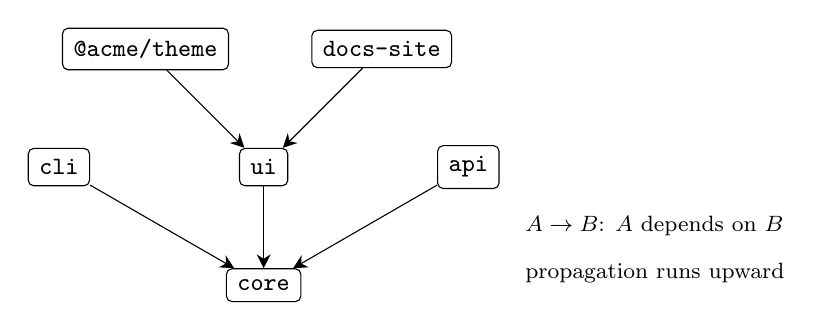
\begin{tikzpicture}[
    >={Stealth[width=5pt,length=5pt]},
    pkg/.style={draw,rounded corners=2pt,inner sep=4pt,font=\small\ttfamily},
    every edge/.style={draw,->}]
  \node[pkg] (core) at (0,0) {core};
  \node[pkg] (cli)  at (-2.6,1.5) {cli};
  \node[pkg] (ui)   at (0,1.5)    {ui};
  \node[pkg] (api)  at (2.6,1.5)  {api};
  \node[pkg] (theme) at (-1.5,3.0) {@acme/theme};
  \node[pkg] (docs)  at (1.5,3.0)  {docs-site};
  \draw[->] (cli)   -- (core);
  \draw[->] (ui)    -- (core);
  \draw[->] (api)   -- (core);
  \draw[->] (theme) -- (ui);
  \draw[->] (docs)  -- (ui);
  \node[font=\footnotesize,anchor=west] at (3.2,0.75)
    {$A \rightarrow B$: $A$ depends on $B$};
  \node[font=\footnotesize,anchor=west] at (3.2,0.15)
    {propagation runs upward};
\end{tikzpicture}
\caption{The running workspace of \cref{ex:workspace}. Distances from
$S=\{\code{core}\}$ are $\dist{S}{\code{cli}} = \dist{S}{\code{ui}} =
\dist{S}{\code{api}} = 1$ and $\dist{S}{\code{docs-site}} =
\dist{S}{\code{@acme/theme}} = 2$.}
\label{fig:workspace}
\end{figure}

\begin{definition}[distance, \spec{9.2}]
\label{def:dist}
For $S \subseteq \Pkgs$ and $d \in \Pkgs$, $\dist{S}{d}$ is the least $n$ for
which there are $p_0 \in S$ and $p_1,\dots,p_n = d$ with $p_{i+1} \in
\Dep{p_i}$ for all $i$, and $\infty$ if no such chain exists. Note
$\dist{S}{d} = 0$ exactly when $d \in S$.
\end{definition}

\subsection{Bumps and versions}

\begin{definition}[bumps, \spec{7.1}, \spec{9.1}]
\label{def:bump}
$\Bumps = \{\bnone, \bpatch, \bminor, \bmajor\}$ ordered
$\bnone < \bpatch < \bminor < \bmajor$. Being a finite chain, $(\Bumps, \leq)$
is a join-semilattice with least element \bnone{} and join $\sqcup = \max$.
\end{definition}

The whole of \spec{9.1}'s ``bumps accumulate'' is the statement that the
combining operator is this join. Two consequences that \SPEC{} states
separately are then immediate and are used without further comment: combination
is associative, commutative and idempotent, so the order in which contributions
are gathered cannot matter; and $x \sqcup y \geq x$, so propagation can only
ever raise a package's bump, never lower or replace a direct decision.

\begin{definition}[versions and channels, \spec{11.1}--\spec{11.4}]
\label{def:version}
\Vers{} is the set of SemVer 2.0.0 versions with SemVer precedence. $\Chans =
\{\stable\} \cup \mathcal{N}$ for a set $\mathcal{N}$ of channel names.
$\chanof{v} = \stable$ if $v$ carries no prerelease identifier, and otherwise
the first (alphanumeric) prerelease identifier of $v$. $\coreof{v}$ is the
\texttt{major.minor.patch} triple of $v$ and $\cntof{v}$ the numeric counter of
a prerelease. $\applyb{v}{b}$ applies bump $b$ to $v$, with $\applyb{v}{\bnone}
= v$.
\end{definition}

\subsection{State}

Everything above is fixed by \Head{} and the configuration. Exactly one thing
changes from run to run, and isolating it is what makes the guarantees provable
as statements about a sequence.

\begin{definition}[engine state, \spec{13.2}, \spec{12.3}]
\label{def:state}
A state \st{} is a finite set of release tags $(p, v, c) \in \Pkgs \times \Vers
\times \Cmts$ with $c \anc \Head$. States are ordered by inclusion,
$\st \leq \st'$ iff $\st \subseteq \st'$. From \st{}:
\begin{itemize}
  \item $\base{\st}{p}$ is the highest-precedence version among the tags of $p$
    in \st{}, undefined if there are none;
  \item $\basec{\st}{p}$ is the commit of that tag;
  \item $\stbase{\st}{p}$ is the highest-precedence non-prerelease version among
    them, and $\stcommit{\st}{p}$ its commit.
\end{itemize}
Where $\base{\st}{p}$ is undefined, $\chanof{\base{\st}{p}} = \stable$ by
convention (\spec{11.1}): a never-released package is graduated by nothing and
is put on a train by any directive naming it.
\end{definition}

The baseline functions additionally assume a unique highest-precedence
reachable tag for each package and each stable baseline. States with tied
precedence and different commits need a specified tie rule and are outside
this proof's domain. Operational lock and temporary refs are not release tags
and are not members of $\st$.

That release-tag states only ever grow is not an assumption about tidy operators; it is
normative. \spec{19.1} forbids moving or deleting a pushed tag and \spec{12.4}
makes tags authoritative over manifests, because a tag is the record that a leg
of the transaction completed and an unwritten-back or rewritten record is
exactly what makes a saga unrecoverable.

\begin{definition}[train and undelivered windows, \spec{13.3}]
\label{def:window}
\begin{equation}
  \Win{\st}{p} \;=\; \Rch{\Head} \setminus \Rch{\stcommit{\st}{p}},
  \label{eq:window}
\end{equation}
and $\Win{\st}{p} = \Rch{\Head}$ when $p$ has no stable baseline in \st{}.
The undelivered window is
\[
  \Winf{\st}{p}=\Win{\st}{p}\setminus\Rch{\basec{\st}{p}},
\]
with an empty subtracted set when $p$ has no baseline tag.
\end{definition}

$\Win{\st}{p}$ is the train window used to aggregate a prerelease target from
its stable base. $\Winf{\st}{p}$ is the fresh-admission window for direct
work, corrections, channels, and propagation to dependent $p$. For a stable
baseline they coincide; on a train they must not be conflated.

\begin{example}[windows]
\label{ex:window}
Let the history be $c_0 \to c_1 \to c_2 = \Head$ with $\st_0$ of
\cref{ex:workspace}, where the tags sit at $c_0$. Then
\[
  \Win{\st_0}{\code{core}} = \{c_1, c_2\},
  \qquad
  \Win{\st_0}{\code{docs-site}} = \{c_0, c_1, c_2\},
\]
the second because a package with no stable baseline has the whole reachable
history pending: \spec{12.5} makes an unreleased package's first release
account for everything, which is also why adopting the engine on an existing
repository does not need a migration step.
\end{example}

\begin{remark}[the window is measured from the last \emph{stable} tag]
\label{rem:stable-window}
This is deliberate and it serves \spec{11.4}: a package on a prerelease train
must accumulate every commit since its last \emph{stable} release, because the
train's target version is recomputed from the stable baseline on every run so
that a breaking change arriving mid-train moves the whole train. The
consequence, which \cref{sec:obligations} returns to at length, is that a
commit already published in a prerelease of $p$ is still a member of
$\Win{\st}{p}$.
\end{remark}

\subsection{Units}

\begin{definition}[units, \spec{4.4}, \spec{13.4}, \spec{13.4b}]
\label{def:unit}
\Units{} is the set of units carried by commits in $\bigcup_{p}\Win{\st}{p}$,
after parsing (\spec{20}), scope resolution (\spec{6}) and the application of
corrections (\spec{13.4b}). For $u \in \Units$:
$\cof{u} \in \Cmts$ is its commit; $\scopef{u} \subseteq \Pkgs$ its resolved
scope-set; $\bumpof{u} \in \Bumps$ the bump its type and \code{!} map to; and
its directives are
\[
  \pbump{u} \in \Bumps,\quad
  \pdepth{u} \in \mathbb{N} \cup \{\infty\},\quad
  \pscope{u} \subseteq \Pkgs,\quad
  \pchan{u},\quad
  \pcdepth{u},\quad
  \pcscope{u} \subseteq \Pkgs,
\]
where $\pbump{u}$ is the \emph{effective} propagated bump: the value the unit
states, or $\bumpof{u}$ where it states \code{inherit}. The two axes default
differently and the asymmetry is deliberate (\spec{8.1}). \code{Propagate}
defaults to \bpatch, not to \code{inherit}: a dependent reached by propagation
has had a dependency change under it but no change to its own public API, so
\bpatch{} is the honest signal, and \code{feat(core)\^{}} therefore gives its
consumers a patch rather than a minor. \code{Propagate-Channel} defaults to
\code{inherit}, since a channel is not a quantity that can be understated.
Both defaults apply only once the corresponding depth is non-zero, and both
depths default to $0$ (\spec{8.3}, \spec{8.3a}): a unit that says nothing
releases its own packages and nothing else. $\pchan{u}$ is a channel value: a
name, \stable, \code{inherit}, \code{none}, or a transition
$\langle f \to t\rangle$.
\end{definition}

Taking corrections as already applied is what \spec{13.4b} prescribes: it
requires \code{Edits} and \code{Deletes} to be resolved into the tuple stream
before cancellation runs, and notes that every later phase operates on the
corrected stream, which downstream phases cannot distinguish from one that was
authored that way.

\begin{remark}[the corrected stream depends on \st{}]
\label{rem:corrections}
It does not follow, and \spec{13.4b} does not claim, that the stream is
independent of the state. A correction reaches only \emph{undischarged} work:
it applies to a $(\text{package}, \text{unit})$ pair only while that package's
window still contains the target commit, and once the package has released the
target the correction is a no-op for it (\diag{W209}, \spec{7.4.2}). So
$\Units{}$ is properly a function $\Units_{\st}$, and a record suppressed by a
\code{Deletes} for a package returns to the stream for that package once the
package releases. This matters in exactly one place, and it is the same place
that a lapsed cancellation matters: \cref{ob:g5}. Everywhere else the two
readings coincide, because a released package's own window is empty and its
direct contribution is therefore already spent, so the notation
$\Units{}$ is kept unindexed below.
\end{remark}

\begin{definition}[suppression and source packages, \spec{13.4a}]
\label{def:sources}
$\canc{c}{p}$ holds when $c$ is an ancestor-or-self of some \code{cancel} commit
whose resolved scope contains $p$ (\spec{10.3}); $\held{p}$ holds when $p$'s
effective \code{Release-As} directive is \code{none} (\spec{13.6a}). Both are
computed from the corrected stream, \Head{}, configuration, and release-tag state. They are constant across retries only where the retry invariant says those inputs remain fixed. Write
\[
  \disch{\st}{p}{c} \;\equiv\; c \notin \Winf{\st}{p},
\]
and then
\[
  \srcp{\st}{u} \;=\;
    \bigl\{\, p \in \scopef{u} \;:\;
       \disch{\st}{p}{\cof{u}} \;\lor\;
       \lnot\bigl(\canc{\cof{u}}{p} \lor \held{p}\bigr) \,\bigr\}.
\]
\end{definition}

The disjunction is the normative content of \spec{13.4a}: suppression applies
only to \emph{undischarged} work. Once $p$ has published the version carrying
$u$, the artefact its consumers are owed is public, and neither a later
\code{cancel} (a no-op, \diag{W170}) nor a later hold may retroactively strand
those consumers. \Cref{ob:g5} shows that this clause, and not the traversal, is
where \G{5} is decided.

\subsection{Runs}

\begin{definition}[plan]
\label{def:plan}
Given \st{}, the release computation of \spec{13} yields the bumps
$\dirb{\st}{p}$ and $\propb{\st}{p}$ (\cref{def:direct,def:propagated}), the
channels $\chanres{\st}{p}$ (\cref{def:channels}), and
$\effb{\st}{p} = \dirb{\st}{p} \sqcup \propb{\st}{p}$. The plan is
\begin{align*}
  \plan{\st} \;=\; \bigl\{\, p \in \Pkgs \;:\;
    &\lnot\held{p} \;\land\;
    \bigl(\effb{\st}{p} \neq \bnone \\[-1mm]
    &\;\lor\; \chanres{\st}{p} \neq \chanof{\base{\st}{p}}
    \;\lor\; p \text{ has an applicable exact } \code{Release-As} \\[-1mm]
    &\hspace{35mm}\text{in }\Winf{\st}{p} \bigr) \,\bigr\},
\end{align*}
each $p \in \plan{\st}$ carrying the version $\vers{\st}{p}$ of \spec{13.9}. The fresh bumps above decide whether work is newly admissible; they are not by themselves the prerelease target. On a train, the intended calculation aggregates the surviving corrected units in $\Win{\st}{p}$ from the stable baseline, including work already delivered to an earlier prerelease. For graduation, the model applies the specific rule of \spec{11.5}: publish that same train target without a prerelease suffix. The generic summary in \spec{13.9} is inconsistent with this rule; \cref{ob:graduation} records the textual obligation.
\end{definition}

\begin{remark}[\plan{\st} is the released set, not the printed one]
\label{rem:plan-held}
\spec{13.9} computes a would-be version for a held package too, and \spec{13.6a}
requires the engine to report it (\diag{W154}) so that the number needed to lift
the hold is available without hand computation. That reported entry is part of
what an operator calls ``the plan'', but it is not a release: \spec{13.10}
excludes it. \plan{\st} above is the released set, which is why \cref{thm:g6}
needs no exception for holds and why the convergence check of \spec{19.6} states
one: the two are reading the same word differently, and only \spec{19.6}'s
reading has to be told about held packages.
\end{remark}

\begin{definition}[run, \spec{19.1}--\spec{19.3}]
\label{def:run}
A run from \st{} is parameterised by a set $F \subseteq \plan{\st}$ of
publishes that fail. It induces the blocked set
\begin{align*}
  B \;=\; \{\, p \in \plan{\st}\setminus F \;:\;
    &\ p \text{ transitively depends on some } q \in F \\[-1mm]
    &\ \text{over } \code{publish.blockingKinds} \,\},
\end{align*}
publishes $\plan{\st} \setminus (F \cup B)$ in the order of \spec{19.2}, and
yields
\[
  \Run{\st}{F} \;=\; \st \;\cup\;
  \bigl\{\,(p, \vers{\st}{p}, \Head) \;:\; p \in \plan{\st}\setminus(F\cup B)\,\bigr\}.
\]
\end{definition}

Three features of this definition carry weight later.

$F$ is chosen adversarially and independently on each run. The guarantees are
claims about \emph{every} failure schedule, not about a well-behaved one; a
proof that appeals to what usually fails proves nothing about a system whose
purpose is to survive what does not usually happen.

Every tag is written at \Head{}, never at the commit the work arrived in
(\spec{19.1}). This is what makes \cref{lem:window} a two-case statement rather
than an argument about which commits a tag covers.

A package is tagged if it is released, whatever its publish target, including
targets of \code{none} that upload nothing (\spec{13.10a}). \Cref{prop:tagall}
shows this is forced: the alternative is a permanent hole in \G{6}.

\begin{definition}[run sequence]
\label{def:seq}
A \emph{run sequence} at \Head{} is $\st_1 \leq \st_2 \leq \cdots$ with
$\st_{k+1} = \Run{\st_k}{F_k}$ for some $F_k \subseteq \plan{\st_k}$. By
\cref{def:run} it is monotone: $\st_k \subseteq \st_{k+1}$.
\end{definition}

\section{Propagation}
\label{sec:propagation}

This section transcribes \spec{9.2}, the three-phase procedure that assigns
each package a propagated channel, resolves every package's channel, and then
assigns propagated bumps. The phase order is forced: phase 3 reads what phase 2
produces, and \spec{9.2} forbids fusing them.

\subsection{The procedure, as written}

The pseudo-code is reproduced from \spec{9.2} unchanged, so that a reader can
diff it against \code{SPEC.md}. The definitions that follow are its
clauses, one by one.

\begin{speccode}[fontsize=\footnotesize]
propagate(units, graph, held, W):
    edges = graph.restrictedTo(config.propagation.kinds)          # §8.4

    # ---------- shared, computed once ----------
    # sourcePackages is a pure function of the unit (§13.4a) and both passes read it.
    # Computing it inside each pass evaluates it twice for every unit carrying both axes.
    src = { u: sourcePackages(u) for u in units }                 # §13.4a

    # ---------- phase 1: channel axis ----------
    chan = {}                                   # package -> (channel, commit, unitIndex)
    for u in units:
        if u.channelDepth == 0:                     continue      # §8.3a: default
        if u.propagateChannel == none:              continue
        sources = src[u]
        if sources is empty:                        continue
        c      = commitOf(u)                                      # loop-invariant
        pscope = resolve(u.propagateChannelScope)                 # §8.5a: resolved once,
        origin = UNCOMPUTED                                     # memoized on first admitted target
        for (d, level) in reach(edges, sources, u.channelDepth):  #   never per target
            if d not in pscope:                           continue
            if c not in Wfresh(d):                             continue # admission, §13.4a
            if cancelledFor(c, d):                        continue # §13.5a
            if u.propagateChannel == 'inherit' and origin == UNCOMPUTED:
                origin = originChannel(u)
            v = propagatedChannelFor(u, d, origin)                 # §9.3; origin computed once
            if v is NONE:                                 continue
            chan[d] = newerOf(chan[d], (v, u))                     # W160 on conflict

    # ---------- phase 2: channel resolution ----------
    channel = resolveChannels(chan, units)                         # §13.8

    # ---------- phase 3: bump axis ----------
    prop = {}                                   # package -> bump
    prov = {}                                   # package -> set of origin packages
    for u in units where bumpOf(u) != none:
        b = (u.propagate == 'inherit') ? bumpOf(u) : u.propagate
        if b == none or u.depth == 0:                continue
        sources = src[u]
        if sources is empty:                        continue
        c       = commitOf(u)
        pscope  = resolve(u.propagateScope)                        # §8.5: once per unit
        # §9.3a resolvability depends only on the unit's sources, so it is decided here,
        # once, and reduces to membership in the distinct source-channel set per target.
        srcChan   = { channel[P] : P in sources }                  # §9.3a
        anyStable = 'stable' in srcChan
        for (d, level) in reach(edges, sources, u.depth):
            if d not in pscope:                           continue
            owed = { P in sources : not delivered(P, c, d) }    # admission, §13.4a
            if owed is empty:                             continue
            if cancelledFor(c, d):                        continue
            if not (anyStable or channel[d] in srcChan):  continue # §9.3a, W208
            prop[d] = max(prop[d], b)
            prov[d] = prov[d] | owed
    return prop, prov, chan
\end{speccode}

The two axes admit differently, and the difference is the subject of this
report's revision. Phase 1 tests \code{c not in Wfresh(d)}: a dependent is
reached on the channel axis if and only if it has not itself released past the
commit carrying the unit. Phase 3 tests \code{owed is empty}: a dependent is
reached on the bump axis if and only if some source of the unit has not yet
\emph{delivered} that commit to it (\cref{def:delivery}). The two coincide
except for a dependent that released past the commit before its source did
(\cref{lem:deliv-window}), and \code{prov[d]} records exactly the owed
sources.

\subsection{The traversal}

\begin{definition}[reach, \spec{9.2}]
\label{def:reach}
For $S \subseteq \Pkgs$ and $\ell \in \mathbb{N}\cup\{\infty\}$,
\[
  \reachset{S}{\ell} \;=\;
  \{\, d \in \Pkgs \setminus S \;:\; \dist{S}{d} \leq \ell \,\},
\]
and each $d \in \reachset{S}{\ell}$ carries the level $\dist{S}{d}$.
\end{definition}

\begin{speccode}
reach(edges, sources, depth):
    frontier = sources
    seen     = set(sources)                     # a unit never reaches its own packages
    out      = {}                               # package -> level
    for level in 1 .. depth:                    # 'all' => until frontier is empty
        next = {}
        for p in frontier:
            for d in edges.dependentsOf(p):
                if d in seen: continue
                seen.add(d); next.add(d)
        if next is empty: break
        for d in next: out[d] = level
        frontier = next
    return out
\end{speccode}

\begin{lemma}[the traversal computes \cref{def:reach}]
\label{lem:reach}
On termination, \code{out} has domain $\reachset{S}{\ell}$ and
$\code{out}[d] = \dist{S}{d}$.
\end{lemma}

\begin{proof}
Standard breadth-first search from the set $S$, seeded at level $0$. By
induction on \code{level}: \code{frontier} at the start of iteration $n$ is
exactly $\{d : \dist{S}{d} = n-1\} \setminus S$ for $n>1$ and $S$ for $n=1$,
because \code{seen} contains precisely the packages at distance $\leq n-1$
(together with $S$ at level zero), and a package first enqueued at iteration $n$ has a chain of
length $n$ from $S$ and none shorter. Membership of \code{seen} is tested
before insertion and never cleared, so each package is assigned at most one
level, its least. The loop runs for $\ell$ iterations or until the frontier is
empty. Seeding $\code{seen} = S$ removes $S$ from the output, which is
\cref{def:reach}'s $\Pkgs \setminus S$.
\end{proof}

Three properties recorded by \spec{9.2} are visible in this statement and are
used repeatedly below. Depth is shortest-path, so a package reachable at both
depth $1$ and depth $3$ is included by \code{+1}. Depth is measured from the
originating source set as a whole and never recomputed from an intermediate
package, so a unit written \code{+1} reaches exactly the direct consumers of its
own packages in every run, whatever released in between. And a package reached
by several paths is visited once, so a diamond does not double-count.

\begin{example}[depth, on \cref{fig:workspace}]
\label{ex:reach}
Take $S = \{\code{core}\}$, the source set of a unit scoped \code{(core)}:

\begin{center}\small
\begin{tabular}{@{}L{2.6cm}L{5.4cm}L{4.6cm}@{}}
\toprule
Written & $\reachset{S}{\ell}$ & Note \\
\midrule
\code{feat(core)} & $\emptyset$ & $\ell = 0$, the default \\
\code{feat(core)\^{}} & $\{\code{cli},\code{ui},\code{api}\}$ & direct consumers \\
\code{feat(core)+2} & $\reachset{S}{1} \cup \{\code{docs-site},\code{@acme/theme}\}$ & two edges out \\
\code{feat(core)\^{}\^{}} & the same set & $\ell = \infty$; the graph is only two deep \\
\bottomrule
\end{tabular}
\end{center}
Now take the two-package source set $S' = \{\code{core},\code{ui}\}$, as a unit
scoped \code{(core,ui)} would have. Then $\reachset{S'}{1} =
\{\code{cli},\code{api},\code{docs-site},\code{@acme/theme}\}$: \code{ui} is
\emph{absent} although it is a dependent of \code{core} at distance $1$,
because \cref{def:reach} removes the whole of $S'$. The unit bumps \code{ui}
directly, and a package is never both a direct and a propagated target of the
same unit. \Cref{prop:bucket} is about exactly this clause.
\end{example}

\begin{remark}[self-exclusion is per unit]
\label{rem:selfex}
$\reachset{S}{\ell}$ excludes all of $S$, not merely the source a given path
started from. This is what stops a unit from propagating to a package it
already bumps directly. It is also the clause that makes the bucketed traversal
of \spec{13.11} unsound if transcribed naively; see \cref{prop:bucket}.
\end{remark}

\subsection{Phase 1: the channel axis}

\begin{definition}[proposed channel, \spec{9.3}]
\label{def:propchan}
For a unit $u$ and package $d$, let $cur = \chanof{\base{\st}{d}}$ (\stable{}
if $d$ has no baseline). Then $\mathrm{pcf}_{\st}(u,d) \in \Chans \cup
\{\NONE\}$ is:
\begin{itemize}
  \item if $\pchan{u}$ is a transition $\langle f \to t \rangle$: \NONE{} if
    $f = t$ (\diag{W207}); \NONE{} if $cur$ does not match $f$, where $f = *$
    matches any $cur \neq \stable$ and otherwise $f$ matches only $cur = f$;
    else $target = t$;
  \item otherwise $target$ is $\pchan{u}$, or the origin channel of $u$ where
    that is \code{inherit}; and if $target = \stable$ while $cur \neq \stable$,
    the result is \NONE{} (\diag{W200}: a propagated channel never graduates
    implicitly);
  \item in either case, if $target = cur$ the result is \NONE{} (\diag{W199});
    otherwise it is $target$.
\end{itemize}
The origin channel of $u$ is the channel $u$'s own \code{Channel} directive
assigns to its sources if it carries one, and otherwise
$\chanof{\base{\st}{p}}$ for its sources $p$, taking the value of the
byte-wise least name if they disagree (\diag{W160}).
\end{definition}

The final clause complements the target \Winf{} admission gate: it compares
$target$ against the package's \emph{baseline} channel rather than against
anything computed in the current run. This no-op check is the other premise of
\G{7}, and \cref{thm:g7} is its consequence.

\begin{definition}[phase 1 output, \spec{9.2}]
\label{def:phase1}
$\mathrm{prop}\chi_{\st}(d)$ is the value $\mathrm{pcf}_{\st}(u,d)$ of the
$\prec$-greatest unit $u$ (newest commit first, then last unit within a commit,
\spec{11.6}) satisfying: $\pcdepth{u} \neq 0$; $\pchan{u} \neq \code{none}$;
$\srcp{\st}{u} \neq \emptyset$; $d \in \reachset{\srcp{\st}{u}}{\pcdepth{u}}$;
$d \in \pcscope{u}$; $\cof{u} \in \Winf{\st}{d}$; $\lnot\canc{\cof{u}}{d}$; and
$\mathrm{pcf}_{\st}(u,d) \neq \NONE$. It is undefined if no unit qualifies.
\end{definition}

The channel axis keeps $\cof{u} \in \Winf{\st}{d}$ as its admission because a
channel is carried by the units and needs no release of the source
(\spec{13.4a}, \G{7}); it has no notion of delivery.

\subsection{Phase 2: channel resolution}

\begin{definition}[channel resolution, \spec{13.8}]
\label{def:channels}
For every $p \in \Pkgs$, whether or not it will be released, let $base =
\chanof{\base{\st}{p}}$ and let $D_{\st}(p)$ be the value proposed by the
$\prec$-greatest unit $u$ with $p \in \scopef{u}$, $\cof{u} \in \Winf{\st}{p}$,
$\lnot\canc{\cof{u}}{p}$, that carries a \code{Channel} directive proposing
something for $p$ (a transition matching $base$, or a value differing from
$base$; a directive proposing nothing is not a competitor and does not count
towards \diag{W186}). Then
\[
  \chanres{\st}{p} \;=\;
  \begin{cases}
    D_{\st}(p) & \text{if defined,}\\
    \mathrm{prop}\chi_{\st}(p) & \text{else if defined,}\\
    base & \text{otherwise.}
  \end{cases}
\]
\end{definition}

A direct directive beats every propagated one regardless of age; among direct
directives, and separately among propagated ones, the newest commit wins and
then the last unit within it. A package named by nothing keeps its baseline
channel, which is why an established train needs no directives to stay
together.

\subsection{Phase 3: the bump axis}

\begin{definition}[resolvability, \spec{9.3a}]
\label{def:resolvable}
$\srcch{\st}{u} = \{\chanres{\st}{p} : p \in \srcp{\st}{u}\}$ and
\[
  \resolv{\st}{u}{d} \;\equiv\;
  \stable \in \srcch{\st}{u} \;\lor\; \chanres{\st}{d} \in \srcch{\st}{u}.
\]
\end{definition}

A bump is a claim that the dependent has something new to pick up, and across a
channel boundary the claim is false: a stable consumer resolves a
beta-releasing dependency by its stable range exactly as before, so a
republished consumer would contain byte-for-byte what its predecessor
contained. Suppression is reported per suppressed pair as \diag{W208}. Note
that \code{srcChan} in the pseudo-code is computed over the whole source set,
not over the owed sources; \cref{sec:duality} returns to this.

\begin{example}[a caret that reaches and does not bump: \SPEC{} vector 95]
\label{ex:resolvable}
The unit \code{feat(core)\^{}\%beta: x} on \cref{fig:workspace}. The \code{\%}
puts \code{core} on \code{beta}; the \code{\^{}} reaches
$\{\code{cli},\code{ui},\code{api}\}$. Phase 2 leaves the three consumers where
their baselines put them, on \stable, so
\[
  \srcch{\st}{u} = \{\code{beta}\},\qquad
  \stable \notin \srcch{\st}{u},\qquad
  \chanres{\st}{\code{cli}} = \stable \notin \srcch{\st}{u},
\]
and \cref{a:resolvable} fails for every one of them: three \diag{W208}
diagnostics, and $\plan{\st} = \{\code{core}\}$ alone. The caret was honoured
and reached its targets; what it would have delivered is not resolvable by
them. Writing \code{feat(core)\^{}\%beta++1} instead moves the same three onto
\code{beta} in phase 1, so $\chanres{\st}{\code{cli}} = \code{beta} \in
\srcch{\st}{u}$ and all four packages release, which is the form that keeps a
train installable as a set.
\end{example}

\begin{definition}[admission, \spec{9.2}, \spec{13.4a}]
\label{def:admission}
For $u \in \Units$ and $d \in \Pkgs$, $\admit{\st}{u}{d}$ holds iff all of:
\begin{enumerate}[label=(A\arabic*),leftmargin=3.2em]
  \item $\bumpof{u} \neq \bnone$, $\pbump{u} \neq \bnone$, $\pdepth{u} \neq 0$;
    \label{a:live}
  \item $\srcp{\st}{u} \neq \emptyset$ and
    $d \in \reachset{\srcp{\st}{u}}{\pdepth{u}}$; \label{a:reach}
  \item $d \in \pscope{u}$; \label{a:scope}
  \item $\owed{\st}{u}{d} \neq \emptyset$; \label{a:window}
  \item $\lnot\canc{\cof{u}}{d}$; \label{a:cancel}
  \item $\resolv{\st}{u}{d}$. \label{a:resolvable}
\end{enumerate}
\end{definition}

\begin{definition}[propagated and direct bumps, \spec{13.6}, \spec{13.7}]
\label{def:propagated}
\label{def:direct}
\begin{align*}
  \propb{\st}{d} &= \bigsqcup \{\, \pbump{u} \;:\; u \in \Units,\ \admit{\st}{u}{d} \,\}, \\
  \dirb{\st}{p} &= \bigsqcup \{\, \bumpof{u} \;:\; p \in \srcp{\st}{u} \cap \scopef{u},\
     \cof{u} \in \Winf{\st}{p} \,\},
\end{align*}
both empty joins being \bnone. Then $\effb{\st}{p} = \dirb{\st}{p} \sqcup
\propb{\st}{p}$.
\end{definition}

\Cref{a:window} is the load-bearing clause of the entire design, and it is
worth being explicit about what it is and is not. It tests the \emph{target's}
position against its \emph{sources'} releases: $d$ is admitted while some
source has not delivered $\cof{u}$ to it. It does not test the source's window,
and it does not test the target's window either. \spec{13.7a} shows what each
of the other readings costs. With retention governed by the source's window, a
dependent whose publish failed while its provider's succeeded is silently
orphaned, permanently one patch behind a dependency it declares, with no
diagnostic, because from the engine's point of view nothing is pending. With
admission governed by the target's window, the rule of CCME 2.0.0, the same
orphan is reached from the other side: a dependent that proceeded past the
commit on a cause of its own while its provider failed is owed nothing once
the provider publishes, and keeps the range it reconciled against the old
version. By \cref{lem:deliv-window} the delivery test agrees with the window
test on every target that has not released past $\cof{u}$; it differs only on
a target that has, where it asks the finer question. Every guarantee in
\cref{sec:guarantees} rests on \cref{a:window} being this test, and
\cref{thm:g2} is where that is used.

\begin{example}[the orphan, from both sides: \SPEC{} vectors 66 and 80d]
\label{ex:orphan}
Both shapes use the history of \cref{ex:window}, $c_0 \to c_1 \to c_2 =
\Head$, with the tags of $\st_0$ at $c_0$ and the unit $u$ =
\code{feat(core)\^{}: streaming reader} at $C = c_2$. So $\scopef{u} =
\{\code{core}\}$, $\bumpof{u} = \bminor$, $\pbump{u} = \bpatch$ (the default of
\cref{def:unit}) and $\pdepth{u} = 1$.

\emph{Provider fails to deliver; the consumer waits} (vector 66). Run 1
evaluates \cref{def:admission} with $\st_0$. All of \code{cli}, \code{ui},
\code{api} lie in $\reachset{\{\code{core}\}}{1}$, none is cancelled, all are
on \stable{} as is \code{core}, and $C \in \Winf{\st_0}{d}$ for each, so by
\cref{lem:deliv-window} $\owed{\st_0}{u}{d} = \{\code{core}\}$, all three are
admitted and
\[
  \plan{\st_0} = \{\code{core},\code{cli},\code{ui},\code{api}\},\qquad
  \vers{\st_0}{\code{core}} = 1.5.0,\quad
  \vers{\st_0}{\code{cli}} = 2.0.1 .
\]
Suppose \code{core}, \code{ui} and \code{api} publish and \code{cli} fails, so
\[
  \st_1 = \st_0 \cup \{\code{core@1.5.0},\ \code{ui@0.9.2},\ \code{api@1.2.1}\}
  \quad\text{at } C.
\]
Run 2 is where the readings of \cref{a:window} separate. Under delivery, the
normative reading, $C \not\anc \basec{\st_1}{\code{cli}} = c_0$, so
$\lnot\deliv{\st_1}{\code{core}}{C}{\code{cli}}$ and
$\owed{\st_1}{u}{\code{cli}} = \{\code{core}\}$: \code{cli} is admitted. Under
the target's window, the reading of CCME 2.0.0, $C \in \Winf{\st_1}{\code{cli}}
= \{c_1, C\}$: \code{cli} is admitted. Under the source's window, the trap,
$C \notin \Win{\st_1}{\code{core}} = \emptyset$: $u$ reaches nobody.
The first two agree, as \cref{lem:deliv-window} says they must for a
\code{cli} that has not released past $C$. For \code{ui}, which has,
$\deliv{\st_1}{\code{core}}{C}{\code{ui}}$ holds with $t = C \anc C =
\basec{\st_1}{\code{ui}}$: nothing is owed, and \code{ui} is out. Under the
normative rule $\plan{\st_1} = \{\code{cli}\}$ at the version run 1 planned,
marked \diag{W193}, and $\plan{\st_2} = \emptyset$. Under the trap
$\plan{\st_1} = \emptyset$ and \code{cli} is never released, on this run or any
later one, with no diagnostic anywhere.

\emph{Consumer gets ahead of its provider} (vector 80d). Let $C$ carry a
second unit $u'$ = \code{feat(cli): y} beside $u$. Then $\dirb{\st_0}{\code{cli}}
= \bminor$, and run 1 plans $\plan{\st_0} =
\{\code{core},\code{cli},\code{ui},\code{api}\}$ with $\vers{\st_0}{\code{cli}}
= 2.1.0$. Suppose \code{core} fails. \code{ui} and \code{api} have no cause of
their own relative to $X = \{\code{core}\}$ and are blocked (\diag{W194});
\code{cli} has one, its direct minor, and \emph{proceeds}
(\cref{def:owncause}): it is published at $2.1.0$ with its manifest reconciled
to \code{core}'s published baseline $1.4.2$, and tagged at $C$. So
\[
  \st_1 = \st_0 \cup \{\code{cli@2.1.0}\ \text{at}\ C\},\qquad
  \Winf{\st_1}{\code{cli}} = \emptyset .
\]
Run 2. \code{core} is planned by its direct minor. For \code{cli}, the window
reading says $C \notin \Winf{\st_1}{\code{cli}}$ and admits nothing: \code{cli}
keeps the range it reconciled against $1.4.2$, is never planned again, and is
one minor behind a dependency it declares, silently. The delivery reading
asks whether \code{core} has delivered $C$ to \code{cli}: $\relc{\st_1}{\code{core}}
= \{c_0\}$ and $C \not\anc c_0$, so $\owed{\st_1}{u}{\code{cli}} =
\{\code{core}\}$, \code{cli} is admitted with $\propb{\st_1}{\code{cli}} =
\bpatch$, and
\[
  \plan{\st_1} = \{\code{core},\code{cli},\code{ui},\code{api}\},\qquad
  \vers{\st_1}{\code{cli}} = 2.1.1,
\]
ordered after \code{core} and blocked if \code{core} fails again. $\st_1$ is
well-formed (\cref{def:wf}): \code{core} would be released at $C =
\basec{\st_1}{\code{cli}}$ and still owes \code{cli}, and \code{cli} is in the
plan after it. Once both are tagged, $\deliv{\st_2}{\code{core}}{C}{\code{cli}}$
holds with $t = C$, nothing is owed, and $\plan{\st_2} = \emptyset$. The plan
of run 2 equals the plan of run 1 although run 1 published a package; that is
the observation \cref{thm:g6} has to accommodate.
\end{example}

\begin{example}[two tags on one commit: \diag{E201}, vector 80d continued]
\label{ex:e201}
Continue the second shape from $\st_1$. Suppose run 2 publishes \code{core},
\code{api} and \code{ui} and \code{cli} fails. Then $\st_2 = \st_1 \cup
\{\code{core@1.5.0}, \code{api@1.2.1}, \code{ui@0.9.2}\}$ at $C$, and now
$\deliv{\st_2}{\code{core}}{C}{\code{cli}}$ holds with $t = C \anc C =
\basec{\st_2}{\code{cli}}$: the ledger reads \code{cli} as served, although
\code{cli@2.1.1} was never published and \code{cli@2.1.0} still names
$1.4.2$. $\owed{\st_2}{u}{\code{cli}} = \emptyset$, $\plan{\st_2} = \emptyset$,
and no later plan at any commit will compute the debt, because two tags on one
commit have no order. This is \cref{prop:loss}: run 2 reports \diag{E201}
for the pair, and the remedy is an explicit \code{Release-As} on \code{cli}
at a later commit. The other route to the same state is prevented rather
than reported: a run 2 in which \code{cli} sat out, held or deselected, would
release \code{core} at \code{cli}'s baseline commit without \code{cli}
following, and \spec{19.3} refuses it before any publication. Had \code{core}
instead published at a later commit $c_3$ in a run \code{cli} sat out, $C$
would stay in $\Wowed{}{\code{core}}{\code{cli}} = \Rch{c_3}\setminus\Rch{c_0}$
(\cref{def:owedwindow}) and the next run would plan \code{cli}'s catch-up.
\end{example}

\begin{remark}[catch-up is not a mode]
There is no separate catch-up pass in this model, and none in the
specification. Catch-up is what the algorithm does when the ordinary rule is
evaluated against the right position (\spec{13.7a}). A ``catch-up release'' is
a label for a release whose entire cause is a propagation from a package not
itself in the run's plan (\diag{W193}); the engine does nothing different to
produce it, and vector 80d's second run is not one, since \code{core} is in
that plan. Catch-up does not widen depth, resurrect a cancelled contribution,
release a held package, change a planned version, or propagate onward from the
catching-up package; each of which is a property of \cref{def:admission}
rather than a rule about catch-up.
\end{remark}

\section{The publish protocol}
\label{sec:protocol}

The guarantees are joint properties of the computation and the protocol that
writes the state the next computation reads. \spec{19} says so explicitly: they
do not survive an implementation that gets this section wrong. Three
obligations are used in the proofs.

\subsection{Tag after, immediately, and always}

\begin{definition}[tagging, \spec{19.1}]
\label{def:tagging}
For each released package: the tag is created at \Head{}; \emph{after} that
package's publish succeeds, never before; \emph{immediately} after it, not
batched to the end of the run; and for every released package whatever its
publish target, including targets that upload no artefact at all.
\end{definition}

Each clause excludes a specific failure. Tagging before publishing makes the
version unrecoverable, because \cref{def:window} will treat it as released.
Batching tags to the end of a run makes a mid-run failure republish everything
already published, which most registries reject outright. Tagging only what
uploads an artefact is the subject of \cref{prop:tagall}.

\subsection{Order}

\begin{definition}[publish order, \spec{19.2}]
\label{def:order}
Let $G$ be the workspace graph restricted to \code{publish.orderKinds} over
\emph{all} packages. Publication proceeds in a topological order of $G$, ties
broken by byte-wise least name, filtered to the plan at the end.
\end{definition}

\begin{proposition}[the order exists, is total, and is deterministic]
\label{prop:order}
\Cref{def:order} is well defined and yields the same sequence on every machine
and in every conforming implementation.
\end{proposition}

\begin{proof}
$G$ is acyclic by \cref{def:graph}, so a topological order exists. Ties are
broken by a total order on names (byte-wise comparison of distinct names), so
the order is total and independent of any container's iteration order. The
filter is applied to a sequence, preserving it.
\end{proof}

\begin{remark}[order over the whole graph, then filter]
\label{rem:filter-last}
Inducing the graph on the planned packages \emph{first} is a defect, not an
optimisation. With $A \to B \to C$ where $B$ has no bump this run (the
common case in any incremental release), the induced subgraph on $\{A, C\}$
has no edge at all, so $A$ may publish against a $C$ that has not published
yet. The constraint is real even though $B$ is not released, because $A$ still
resolves $C$ through $B$ at install time. This is why the model orders over
\Pkgs{} and filters last, and why an implementation detecting a violation must
raise \diag{E197}.
\end{remark}

Order matters for a reason no later run can repair. A dependent published
before its dependency carries a range reconciled against the dependency's old
version, and both land at the same commit, so no ancestry test can tell
afterwards that anything is wrong (\spec{13.7b}). The inconsistency is
undetectable after the fact, which is why it is prevented rather than
diagnosed.

\subsection{Partial failure}

\begin{definition}[blocking, \spec{19.3}]
\label{def:blocking}
On a failure, every package in the plan that transitively depends on the failed
one over \code{publish.blockingKinds} is \emph{blocked} (\diag{W194}): planned,
but not attempted in this run. The closure is computed over the full workspace
graph, so it traverses packages that are not in the plan. Packages that are not
blocked continue to publish.
\end{definition}

Ordering and blocking use different edge-kind sets, and the asymmetry is
deliberate: \code{orderKinds} includes optional dependencies, because an
optional dependency should still be available before its dependent, while
\code{blockingKinds} excludes them, because a missing optional dependency does
not break an install and a missing required one does.

\begin{example}[an infrastructure leg]
\label{ex:terraform}
Nothing in \cref{def:tagging,def:run} requires a publish leg to be a registry
upload. A \code{terraform apply} may be such a leg: its build stage imports the
explicitly configured live resources and writes a plan, and its publish stage
applies that plan before the release tag is written. The tag records that this
version of the configuration completed successfully. It is not Terraform
resource state, does not prove that every live resource was imported, and does
not make applying an arbitrary configuration externally idempotent. Application
builds may overlap the apply; only their publication waits for the
infrastructure publish edge.
\end{example}

\begin{remark}[recorded-success abstraction]
\Cref{def:run} models confirmed successful legs by their tags. It proves
properties of that release ledger, not convergence of an external registry or
infrastructure state. A publish may take effect before its tag is recorded;
then the repository alone is insufficient and \cref{def:reconcile} or a
publish-target-specific idempotence contract is required. Terraform likewise
needs its own state or an explicit, complete import boundary before a plan can
safely describe existing resources.
\end{remark}

\begin{definition}[reconciliation, \spec{19.4}]
\label{def:reconcile}
When a publish fails because the version already exists, the implementation
verifies by registry digest or provenance attestation that the published
artefact is the one this run would have published; if it matches, the publish
counts as successful and the tag is written (\diag{W196}); if it does not
match, or identity cannot be established, the run stops with \diag{E198}.
\end{definition}

This is the one place where the model's ``a publish either succeeds or fails''
abstraction meets a third outcome, that it already happened, and
\cref{def:reconcile} maps it back onto success. Verification is what makes that
safe: without it, adopting a version published by something other than this run
would enrol a foreign artefact into the release lineage, which is a
supply-chain vulnerability rather than a convenience.

\section{Execution: what readiness and placement cost}
\label{sec:execution}

\Cref{sec:protocol} states what must happen before what. This section states
what that costs in wall time, where the tasks may run, and which history each
window ranges over when the packages live in several repositories. The duration
propositions are informative in the sense of \spec{13.11}: they bound
durations of schedules that respect \cref{def:readiness}, and no conforming
implementation is required to attain them. The two optional profiles of
\spec{28} and \spec{27} are transcribed as definitions, with the one invariance
each promises, in \cref{sec:exec-distributed,sec:exec-polyrepo}. Nothing here
extends the theorems of \cref{sec:guarantees}, which are stated for a single
history.

\subsection{Build readiness durations}
\label{sec:exec-durations}

\spec{19.2a} promises a happens-before relation and no duration; \spec{13.11}
nevertheless says what each relation buys when nothing else limits the run.
Throughout, package $i$ has a build of duration $b_i$ and a publication of
duration $p_i$, both fixed; a task starts as soon as its predecessors in the
task graph of \cref{def:taskgraph} have finished and a slot is free; and one
relation is declared on every edge.

\begin{proposition}[the longest path, \spec{13.11}]
\label{prop:exec-longest}
With unlimited build and publication slots a run lasts exactly the longest
path $L$ of its task graph, measured in task durations. A weaker relation
never lengthens it.
\end{proposition}

\begin{proof}
The task graph is acyclic (\cref{prop:readiness-acyclic}), so its tasks can be
taken in a topological order. With unlimited slots a task starts at the
greatest finish time of its predecessors, or at $0$ if it has none, and by
induction along that order its finish time is the longest path ending at it.
The run ends at the greatest finish time, which is the longest path of the
graph. A weaker relation contributes a subset of the edges
(\cref{prop:readiness-acyclic}), so every path of its task graph is a path of
the stronger one's, and the longest is no longer.
\end{proof}

\begin{proposition}[a chain, \spec{13.11}]
\label{prop:exec-chain}
Let packages $1, \dots, n$ form a chain in which package $k+1$ consumes package
$k$, under one relation throughout. With unlimited slots the run lasts
\[
  \sum_{i=1}^{n} (b_i + p_i) \quad\text{under \code{publish}},\qquad
  \max_{1 \le k \le n}\Bigl(\sum_{i=1}^{k} b_i + \sum_{i=k}^{n} p_i\Bigr)
  \quad\text{under \code{build}},
\]
\[
  \max_{1 \le k \le n}\Bigl(b_k + \sum_{i=k}^{n} p_i\Bigr)
  \quad\text{under \code{none}}.
\]
\end{proposition}

\begin{proof}
Under \code{publish}, $\exbuild{k+1}$ waits for $\expub{k}$, so the $2n$ tasks
form one path and the sum is its length. Under \code{build}, the builds form
the path $\exbuild{1} \to \dots \to \exbuild{n}$ and $\exbuild{k}$ ends at
$B_k = \sum_{i \le k} b_i$; the publication of $k$ waits for $\exbuild{k}$ and
for $\expub{k-1}$, so its finish $E_k$ satisfies $E_k = \max(B_k, E_{k-1}) +
p_k$ with $E_0 = 0$. By induction $E_k = \max_{j \le k}\bigl(B_j +
\sum_{i=j}^{k} p_i\bigr)$: the case $k = 1$ is $B_1 + p_1$, and the step is
$\max\bigl(B_k + p_k,\ \max_{j < k}(B_j + \sum_{i=j}^{k-1} p_i) + p_k\bigr)$.
Under \code{none} every build starts at $0$ and $\exbuild{k}$ ends at $b_k$;
the same recurrence with $b_k$ in place of $B_k$ gives the third form. In each
case the run lasts $E_n$ by \cref{prop:exec-longest}.
\end{proof}

\begin{corollary}[equal durations]
\label{cor:exec-equal}
With $b_i = b$ and $p_i = p$ for all $i$, the three forms are $n(b+p)$,
$\max(nb + p,\ b + np)$ and $b + np$. \code{build} saves $(n-1)\min(b,p)$
over \code{publish}, and \code{none} saves a further $(n-1)\max(b-p, 0)$, so
the second saving exists only where builds outlast publications.
\end{corollary}

\begin{proof}
Under \code{build} the maximand $kb + (n-k+1)p$ is affine in $k$, so the
maximum is at $k = 1$ or $k = n$. Under \code{none} the maximand $b + (n-k+1)p$
is greatest at $k = 1$. The differences follow by cases on $b \ge p$.
\end{proof}

\begin{proposition}[fan-out and fan-in, \spec{13.11}]
\label{prop:exec-fan}
For one provider $0$ and consumers $i \ge 1$, each consuming $0$ and nothing
else, the run lasts
\[
  b_0 + p_0 + \max_i (b_i + p_i),\qquad
  b_0 + \max_i\bigl(\max(b_i, p_0) + p_i\bigr),\qquad
  \max_i\bigl(\max(b_i,\ b_0 + p_0) + p_i\bigr)
\]
under \code{publish}, \code{build} and \code{none} respectively. For providers
$i \ge 1$ of one consumer $c$, each consumed by $c$ and nothing else, it lasts
\[
  \max_i (b_i + p_i) + b_c + p_c,\qquad
  \max\bigl(\max_i b_i + b_c,\ \max_i (b_i + p_i)\bigr) + p_c,\qquad
  \max\bigl(b_c,\ \max_i (b_i + p_i)\bigr) + p_c.
\]
\end{proposition}

\begin{proof}
Fan-out. Under \code{publish}, consumer $i$'s build starts at $b_0 + p_0$ and
its publication follows its build, giving $b_0 + p_0 + b_i + p_i$; take the
maximum. Under \code{build}, its build starts at $b_0$ and ends at $b_0 + b_i$,
and its publication waits for that and for $\expub{0}$ at $b_0 + p_0$, giving
$b_0 + \max(b_i, p_0) + p_i$. Under \code{none}, its build ends at $b_i$ and its
publication waits for that and for $b_0 + p_0$. Fan-in. Under \code{publish},
$c$'s build starts when the last provider has published, at $\max_i (b_i +
p_i)$. Under \code{build}, it starts at $\max_i b_i$ and ends $b_c$ later, and
$c$'s publication waits for that and for every provider's publication. Under
\code{none}, $c$'s build ends at $b_c$ and only its publication waits for the
providers. Each is the longest path of \cref{prop:exec-longest}.
\end{proof}

\begin{proposition}[one publication lane, \spec{13.11}]
\label{prop:exec-lane}
Where one owner's publications are serialised (\spec{27.2}, \spec{28.6}) in
the order $1, \dots, n$ of \cref{def:order}, let $e_k$ be the instant the build
of package $k$ ends. Under every relation the run lasts
\[
  \max_{1 \le k \le n}\Bigl(e_k + \sum_{i=k}^{n} p_i\Bigr),
\]
which is at least $\sum_{i} p_i$ whatever the relation, and a weaker relation
only lowers the $e_k$.
\end{proposition}

\begin{proof}
Publication $k$ starts at $\max(e_k, E_{k-1})$, since it waits for its own
build and for the lane, and the lane order agrees with \cref{def:order}, so
every provider of $k$ has published by $E_{k-1}$. The recurrence is that of
\cref{prop:exec-chain} with $e_k$ in place of $B_k$, and the same induction
gives the maximum. The term $k = 1$ is $e_1 + \sum_i p_i \ge \sum_i p_i$. For
the last claim, add the lane edges $\expub{k-1} \to \expub{k}$ to the task
graph; they follow the publish order, which is a topological order of the
workspace graph, so the key of \cref{prop:readiness-acyclic} still increases
along every edge and the graph stays acyclic. With a fixed lane order every
task starts at the greatest finish of its predecessors, and by induction along
a topological order each finish time under a subset of the edges is at most
the finish time under the full set; $e_k$ is such a finish time.
\end{proof}

\begin{proposition}[budgets, \spec{13.11}]
\label{prop:exec-budget}
Let there be $m_b$ build slots and $m_p$ publication slots, and write $W_b =
\sum_i b_i$, $W_p = \sum_i p_i$ and $L$ for the longest path of the task
graph. No schedule finishes before $\max(L,\ W_b/m_b,\ W_p/m_p)$. A schedule
that never leaves a slot of a stage idle while a task of that stage is ready
finishes within $L + W_b/m_b + W_p/m_p$, which is within three times the best
possible. Under budgets a weaker relation can lengthen such a schedule, but
never the best one.
\end{proposition}

\begin{proof}
The lower bound: a schedule contains every path, so it lasts at least $L$; it
performs $W_b$ units of build work on $m_b$ slots, so at least $W_b/m_b$; and
likewise $W_p/m_p$. The upper bound: let the schedule end at $T$ and let $t_1$
be a task finishing at $T$. For $j \ge 1$, while $t_j$ has predecessors, let
$t_{j+1}$ be one that finishes last among them; this gives a chain $t_q \to
\dots \to t_1$ whose total duration is at most $L$. Consider an instant of
$[0, T)$ at which no task of the chain is running. It lies between the finish
of some $t_{j+1}$ and the start of $t_j$ (or before the start of $t_q$), and
at that instant $t_j$ is ready, since its latest predecessor has finished, and
has not started; by hypothesis every slot of $t_j$'s stage is then busy. The
instants at which all $m_b$ build slots are busy total at most $W_b/m_b$, and
those at which all $m_p$ publication slots are busy at most $W_p/m_p$. Hence $T
\le L + W_b/m_b + W_p/m_p$, and each summand is at most the lower bound. For
the last claim, a schedule feasible under a stronger relation is feasible under
a weaker one, so the best weaker schedule is no longer; that a particular
greedy schedule can be longer is \cref{ex:exec-anomaly}.
\end{proof}

The bound is Graham's argument for list scheduling under precedence
constraints~\cite{graham66,graham69}, applied to two stages with separate
budgets; \spec{13.11} does not claim it tight for this shape of graph.

\begin{example}[Graham's anomaly, \spec{13.11}]
\label{ex:exec-anomaly}
Take two build slots and one publication slot, packages $A = (2, 3)$ and $B =
(1, 2)$ where $B$ consumes $A$, and an unrelated $C = (8, 3)$, with ready tasks
taken in the order $A, B, C$. Under \code{build}, $B$'s build is not ready at
$0$: $A$ builds in $[0,2)$ and $C$ in $[0,8)$ on the two slots; $B$ builds in
$[2,3)$; $A$ publishes in $[2,5)$, $B$ in $[5,7)$ once $A$ has published, and
$C$ in $[8,11)$ once its build ends. The run lasts $11$. Under \code{none},
$B$'s build is ready at $0$ and takes the second slot: $A$ builds in $[0,2)$
and $B$ in $[0,1)$, so $C$ builds only in $[1,9)$; $A$ publishes in $[2,5)$,
$B$ in $[5,7)$ and $C$ in $[9,12)$. The run lasts $12$: the consumer's early
build took the slot the long build would have had. A list that preferred $C$
to $B$ at $0$ would finish at $11$ under \code{none} as well, which is the
point: the length depends on the list, not on the relation, and it is why
\spec{19.2a} promises a happens-before relation and no duration.
\end{example}

\begin{example}[an infrastructure chain]
\label{ex:exec-chain}
Let the infrastructure leg of \cref{ex:terraform} be consumed by a backend
consumed in turn by a frontend, with $(b, p)$ in minutes of $(4, 6)$ for the
infrastructure, $(9, 3)$ for the backend and $(12, 2)$ for the frontend. By
\cref{prop:exec-chain}, under \code{publish} the run lasts $10 + 12 + 14 = 36$
minutes; under \code{build} it lasts $\max(4 + 11,\ 13 + 5,\ 25 + 2) = 27$;
under \code{none} it lasts $\max(4 + 11,\ 9 + 5,\ 12 + 2) = 15$. The
publications still run in order in every case, and the frontend's publication
still ends the run.
\end{example}

\subsection{Distributed execution}
\label{sec:exec-distributed}

\spec{28} is an optional execution profile that changes no message syntax and
asserts no speedup. The definitions below transcribe its obligations; the one
proposition is the invariance it promises.

\begin{definition}[nodes and roles, \spec{28.1}]
\label{def:exec-roles}
An execution node is a machine or runner executing the same release engine and
configuration schema; it is distinct from a repository peer. Every node
supports two roles, and one engine provides both. The default role is
\emph{orchestrator}. An explicit \emph{worker} refuses release initiation,
including indirect initiation from a delegated hook, and executes authorised
tasks in an existing run; it never substitutes a locally recomputed plan,
acquires competing release ownership, dispatches to another pool, or
independently finalises a release. An orchestrator-capable node that accepts
a delegated task has only worker authority for it. The node on which CI starts
the release is the run's orchestrator, of which there is one per run; it owns
lock acquisition, the fixed planning input, task allocation, result admission
and release finalisation, and may execute tasks locally under the same rules
as a worker. Workers may be added to every history mode; execution links are
not fleet links and alter neither source discovery nor release scope.
\end{definition}

\begin{definition}[lock, snapshot, plan, assign, \spec{28.3}]
\label{def:exec-input}
Before creating a write-capable run the orchestrator identifies every
participating repository, acquires all release locks in one stable total
order, verifies ownership, and revalidates discovery under those locks; a
changed participant set releases the partial acquisition and acquires the
complete set again. Discovery and compatibility inspection before locking are
read-only, and an unsafe lock bypass is refused. The run input $\exI$ contains
the fixed repository-qualified heads and complete relevant history, the release
records of the authoritative stores as compared under the locks
(\cref{def:records-lock}), the graph, the resolved semantic configuration, the
explicit release options, and the withdrawal inventory and receipts of
\spec{26}. The semantic release plan is the pure function $\exPlan(\exI)$.
Node placement configuration is not semantic input: worker count, placement,
completion order, wall-clock time, run identifiers and transport branch names
do not change $\exPlan(\exI)$. A plan digest is computed over a canonical
serialisation of semantic input and plan content, and transient execution
identity is bound separately. The orchestrator derives a task graph from the
plan, including preparation, tests, builds, transfers, publications and
recording gates; a task is placed only on a compatible node and only when its
exact prerequisites are available; the schedule need not be deterministic.
Where a package's stages may be placed is execution policy declared beside
\cref{def:readiness} and, like it, no part of the plan. Every reconciliation
that writes a shared manifest or lockfile is an explicit task under the
orchestrator's authority, serialised per shared file; each admitted result is
one prepared input state, builds fan out only from an admitted state, and
every build binds the state it consumed. An assignment identifies the run,
plan digest, task, attempt, ownership generation, repository-qualified source
object identifiers, effective configuration and command environment,
toolchain and platform requirements, input receipts, permitted writes and
outputs; workers authenticate the assigning orchestrator and the assignment's
integrity; duplicate delivery is recognised; only one attempt is authorised
to perform a given external side effect; and a task receipt is execution
evidence, never a release record.
\end{definition}

\begin{proposition}[placement invariance]
\label{prop:exec-placement}
For a fixed input $\exI$, the plan $\plan{\st}$, the versions
$\vers{\st}{\cdot}$ and the publish order of \cref{def:order} do not depend on
the placement of tasks, on the number of nodes, or on the order in which tasks
complete.
\end{proposition}

\begin{proof}
By \cref{thm:determinism} the plan, the versions and the planned publish
order are functions of $(\st, \Head, \mathrm{config})$ alone. $\exI$ fixes all
three: \st{} is the set of release records compared under the locks
(\cref{def:records-lock}), \Head{} is the fixed repository-qualified head, and
the configuration is the run's resolved semantic configuration. Nothing a node
contributes reaches those arguments: the node-startup settings of \spec{28.2}
(role, capacity, worker links) do not override package policy, planned
versions, commands or inputs; the build readiness relation and the placement
policy are execution policy outside the plan (\cref{def:readiness},
\cref{def:exec-input}); and placement, node count and completion order are
excluded from $\exI$ by \cref{def:exec-input}. A function of fixed arguments
takes one value. Vectors 3 and 5 of \spec{28.8} are this statement.
\end{proof}

\begin{definition}[Git synchronisation branches, \spec{28.4}]
\label{def:exec-branches}
The orchestrator provisions isolated task worktrees and temporary coordination
branches named \code{dispat-worker-<id>-<workinfo>}, created atomically under
\code{refs/heads/}, where \code{<id>} is the node the branch is addressed to
and \code{<workinfo>} carries a date, a kind label and at least 128 bits of
randomness. The name is an untrusted routing hint that lets a node list the
branches addressed to it; the authenticated manifest, not the name,
identifies node, run, task and attempt, and a node rejects a manifest whose
binding disagrees with where it was found. Each acknowledged checkpoint
identifies an exact full object identifier, and a consumer reads only from
that object, never from a tip that can still move; a tip fetched but not read
or verified has not been seen. Ref updates and deletions check the expected
previous object identifier and attempt ownership, so that an update racing
another party's update fails instead of overwriting it. Transport credentials
do not authorise a worker to update native release branches, tags or fleet
settlement refs. A source snapshot may travel without the history behind it,
as a parentless commit or bare tree, because a task's commands may not read
history from a transport checkout. Transport commits are never release intent,
a window boundary, a successful release or an admitted native head; they are
neither merged into a release branch nor made ancestors of release tags, and
only validated release-file changes enter native recording through the
ordinary transaction. Artefact provenance binds the exact source revision and
admitted release-file state used for the build.
\end{definition}

\begin{definition}[outputs as first-class inputs, \spec{28.5}]
\label{def:exec-outputs}
A provider's revision does not make its ignored or generated outputs
available on another machine, so a conforming implementation transports the
outputs a local-output dependency needs, declared ignored and generated files
included; it neither reclones and rebuilds the provider closure on every
consumer node nor pins the connected graph to one worker. A successful build
emits a manifest binding its outputs to the run, plan, task, attempt,
repository-qualified source revision, admitted release-file state, package and
version, toolchain and platform, and input and output digests. Identity is by
content: consumers verify the authenticated manifest, content integrity and
compatibility before their stage becomes ready; installation is atomic at the
task-input boundary; a completed build publishes one admitted output set for
its exact attempt; and a missing, stale, incomplete or incompatible output
fails the prerequisite and is never substituted with registry contents or a
new build under a different input. Bytes travel through the coordination
branch or through immutable content-addressed bundles whose references and
digests are in it; a reference alone is not a transfer. For package edge $B
\to A$ under the \code{build} relation, readiness is the task precedence
$\exbuild{A} \to \mathrm{export}(A) \to \mathrm{verify/materialise}(A
\text{ at } B\text{'s node}) \to \exbuild{B}$; under \code{publish} it
requires $A$'s publication and every applicable recording gate, which local
bytes never replace; under \code{none} the edge carries no output and the two
builds are independent tasks. A provider a consumer reaches only across
\code{none} edges is no input of that consumer and is not prepared for it:
the input closure ends at a \code{none} provider. Task inputs include every
required build dependency, including packages needing no new release and
build-only edges outside the propagation kinds; the task graph is acyclic,
and an unschedulable cycle is an execution-configuration error, never a
reason to change release intent. Verified outputs may be reused across runs
only under a new admission receipt bound to the current run, plan and task
attempt.
\end{definition}

\begin{definition}[publication, recording and recovery, \spec{28.6}, \spec{28.2}]
\label{def:exec-publication}
The orchestrator alone admits results and authorises publication, after the
ordinary test, dependency, settlement and relevant-input checks; it serialises
publication and recording within one owner, a single-history monorepo
included, while isolated builds within that owner may overlap and independent
owners keep their publication concurrency. A worker never moves release
branches, creates release tags, settles peer links or finalises the fleet.
Authorisation to publish is explicit, single-use and bound to one task
attempt: it is issued only after the package's \code{beforePublish} hook has
completed on the executing node and after the relevant-input and lock-ownership
checks, the publisher does not start its command before it has observed the
authorisation for its own attempt, and an authorisation is never reused by
another attempt or for another effect. An authorisation may be bounded in
time, with a start instant after which the publisher does not begin and a
deadline at which the executing node ends the command itself; the bound
limits when an effect may begin and how long it runs, is not an expiry of the
release lock, and authorises no takeover. The orchestrator retains and
verifies lock ownership for the lifetime of all authorised effects, and
assignments and results are bound to its ownership generation. After lock
loss no new effect starts: no further assignment and no further
authorisation. Recording an effect authorised before the loss is not a new
effect and is still attempted, as the create-only record of
\cref{def:tagging}, because a publication left unrecorded is a wedge the next
owner can clear only by \cref{def:reconcile}, and a create-only record cannot
overwrite what a successor wrote. A timed-out worker is not proof that its
publisher stopped: before ownership is handed over, cancellation is
acknowledged with the phase the attempt stopped in, or a fence is enforced
where the effect occurs, or the outcome is reconciled; a generation field
alone fences no registry command, and no takeover expires ownership while the
previous process can still act. Capacity returns only on evidence: an
in-flight attempt retains its reservation until completion, acknowledged
cancellation or safe fencing, a timeout alone frees nothing, and an
assignment no node has claimed holds no capacity and may be withdrawn and
offered again. A worker that fails before publication is retried under a new
attempt without discharging the package; a publication that may have
succeeded is reconciled by \cref{def:reconcile} before another attempt, since
neither a missing reply nor a missing tag proves failure; only the durable
source release record discharges the obligation. Locks are released only after
authorised operations have quiesced or been fenced, in reverse acquisition
order; if that cannot be proved the run fails holding its exclusion and no
record of the uncertain package, which the next run treats as pending. An
attempt never authorised to perform an external effect is fenced by revoking
its coordination ref; an authorised publisher is not. An abandoned run is
findable from its lock, and recovery revokes the run's coordination refs,
settles every authorised attempt without a result, and only then removes the
lock.
\end{definition}

\begin{example}[the required example, \spec{28.7}]
\label{ex:exec-required}
In one large JavaScript repository let $\code{assets} \Rightarrow \{\code{ui},
\code{docs}\} \Rightarrow \code{app}$ denote task precedence: \code{ui} and
\code{docs} consume \code{assets}, and \code{app} consumes both; the package
edges of \cref{def:graph} point the other way. Worker $A$ builds \code{assets}
once and exports its required outputs. Workers $B$ and $C$ receive verified
outputs and build \code{ui} and \code{docs} concurrently. The assigned
\code{app} worker receives both output sets and builds \code{app}.
Publication and source recording then obey \cref{def:order} and the owner
lane of \cref{def:exec-publication}. Neither $B$ nor $C$ rebuilds
\code{assets}, and the \code{app} worker rebuilds neither closure. The
example works without converting the monorepo to a polyrepo or publishing
private intermediate packages solely for transport.
\end{example}

\begin{remark}[the performance boundary, \spec{28.7}]
\label{rem:exec-boundary}
The required gain is the distribution and reuse of dependent builds with
parallel ready branches; universal speedup is not a semantic guarantee. Git
provides source and result transport; it does not schedule tasks, transfer
omitted build products, guarantee compatible environments or make effects
exactly-once. A strictly serial chain retains its critical path, and transfer
and setup overhead can outweigh saved compute on small jobs. Before an
implementation claims a performance gain it compares the same pinned fixture
locally and on several nodes, reporting cold and warm setup, per-node
resources, transfer bytes and time, task execution counts, total work, wall
time, repetitions and variability, and artefact equivalence, with the fixture
and environment identified; skipped or failed trials are not speedups, and
neither source-only dispatch nor duplicated prerequisite compilation is a
distributed-build success.
\end{remark}

\begin{proposition}[list scheduling under placement, \spec{13.11}]
\label{prop:exec-graham}
Let $W_k$ be the summed duration of a run's command tasks, $L_k$ the duration
of its longest precedence chain, and $s$ the task slots usable at once, the
lesser of the summed node capacities and the applicable run-wide stage
limits. No schedule finishes before $\max(L_k,\ W_k/s)$. When slots are
interchangeable and transfers cost nothing, a placement that never leaves a
usable slot idle while a compatible task is ready finishes within $W_k/s +
(1 - 1/s)\,L_k$, which is at most $(2 - 1/s)$ times the best possible. On a
chain $L_k = W_k$ and no number of nodes helps.
\end{proposition}

\begin{proof}
The lower bound is that of \cref{prop:exec-budget} with one stage. For the
upper bound take the chain $t_q \to \dots \to t_1$ of that proof. At every
instant either a chain task runs or all $s$ slots are busy, and in the latter
case the work done off the chain is at most $W_k - L'$ where $L' \le L_k$ is
the chain's length; so the off-chain time is at most $(W_k - L')/s$ and the
makespan at most $L' + (W_k - L')/s = W_k/s + (1 - 1/s)L' \le W_k/s + (1 -
1/s)L_k$. Each of $W_k/s$ and $L_k$ is at most the optimum, giving the factor.
This is Graham's bound for list scheduling under precedence
constraints~\cite{graham66,graham69}. On a chain every task is on the
longest path, so $L_k = W_k$ and the lower bound is $W_k$ for every $s$.
\end{proof}

Neither premise holds in general: nodes differ in platform and speed, and an
output transfer delays the consumer it feeds. \spec{13.11} therefore states no
bound once transfers count and puts the measurement of
\cref{rem:exec-boundary} in its place. The inequality still says what to
expect: once $s \ge W_k/L_k$ the lower bound is $L_k$, so the chain and not the
pool is the limit, and more nodes can only close the gap between a greedy
schedule and $L_k$, which is below a factor of two.

\paragraph{Implementation status.}
The design history of \SPEC{} dated 2026-09-22 records that the dispat
release engine implements the profile in every history mode over the Git
mailbox transport of \cref{def:exec-branches}: every message is a signed tree
on a branch, every transition one compare-and-swap ref update, a worker
polls, and nothing connects to a worker. Builds and publications run on
workers, a publication is delegated only by an explicit placement, a space
that logs in to its registry publishes on the orchestrator, the orchestrator
is one more node of the pool chosen last, and a provider the run does not
release is prepared once per run when a consumer reads its outputs. Outputs
travel as result trees on the branches, with no bundle service, which is
vector 17 of \spec{28.8}. Not implemented, so their conditional vectors do
not apply: reuse of verified outputs across runs (vector 20) and the rollback
profile of \spec{26} (vector 26); the durable mailbox ref and the
history-free snapshot that \spec{28.4} permits are likewise unimplemented, so
a snapshot descending from the planned head carries the repository's whole
history to a mailbox that starts empty. Departures from the profile as
written: the platform check of \spec{28.2} runs before dispatch for the
packages a run releases and, for a prepared provider, at its placement; and
the \code{native-recording-or-lock} class is attached where a distributed run
loses its lock and not yet at the older recording and lock sites. The same
history records that the owed windows of \spec{13.3} and \diag{E201}
(\cref{def:owed-commit}) are not yet implemented, so a consumer that sits out
the run in which its provider releases the owed commit is still stranded in
that engine. What was measured, on which fixtures, is reported in
\cref{sec:evaluation}.

\subsection{Repository-local windows}
\label{sec:exec-polyrepo}

\spec{27} plans one package graph whose packages are owned by several linked
Git repositories. It changes where history and release records are read and
nothing else: the grammar, the bump lattice, the windows, holds,
cancellation, corrections, channel rules, the dependency graph and the
partial-publication rules of \cref{sec:protocol} are unchanged. This
subsection defines the objects the profile adds and states what it promises;
it does not extend the single-history theorems of \cref{sec:guarantees} to
several histories.

\begin{definition}[fleet snapshot and commit identity, \spec{27.2}]
\label{def:exec-fleet}
Before parsing history the engine resolves one immutable map from repository
identity to full commit object identifier, the fixed fleet snapshot; every
participating repository is an initialised, non-shallow checkout at its
pinned commit, and a missing, shallow, moved or ambiguous participant is
\diag{E330}. A commit identity is a pair (repository, full object
identifier); two equal identifier byte strings in different repositories are
incomparable. Commit dates, author dates, modification times, tag creation
dates and fetch order create no ancestry or precedence. The engine reads each
repository's reachable DAG once for the snapshot, preserves native parent
order, and manufactures no synthetic fleet DAG or parent edge. Ancestry,
changed paths, direct pending windows, cancellation barriers, corrections and
\code{Reverts} are evaluated in the repository that owns the commit.
\end{definition}

\begin{definition}[repository-local windows, \spec{27.5}, \spec{27.6}, \spec{27.11}]
\label{def:exec-windows}
For a source repository $r$ with fixed head $h_r$, write $\exRch{r}{x}$ for
the ancestors-or-self of a commit $x$ of $r$, and
\[
  \exafter{r}{x} \;=\; \exRch{r}{h_r} \setminus \exRch{r}{x},
  \qquad
  \exafter{r}{\NONE} \;=\; \exRch{r}{h_r}.
\]
For a consumer package $D$ and a repository $r$, let $s_{D,r}$ be the
revision of $r$ that $D$'s last stable release incorporated and $b_{D,r}$ the
revision of $r$ that $D$'s newest release of any channel incorporated, each
$\NONE$ where no such release exists. $D$'s train and fresh windows over $r$
are
\[
  \exWin{D}{r} \;=\; \exafter{r}{s_{D,r}},
  \qquad
  \exWinf{D}{r} \;=\; \exafter{r}{s_{D,r}} \cap \exafter{r}{b_{D,r}}.
\]
When $r$ owns $D$, the boundaries are the commits of $D$'s own release tags,
and the windows are those of \cref{def:window}. When $r$ does not own $D$,
the boundaries are the positions $D$'s releases prove in $r$, and only these
prove them: a control release checkpoint whose release-commit message names
$D$'s exact tag, changes $D$'s gitlink to the commit peeled from that tag, and
pins the revision of each other repository the release incorporated
(\spec{27.6}); an explicit \code{repositoryBaselines} tuple $(D,
\text{release tag}, r, \text{revision})$, with stable and prerelease tags as
separate entries (\spec{27.6}); or, in the linked peer topology, the route of
fleet links recorded hop by hop from the tree of the release commit that
names $D$'s tag (\spec{27.11}). A matching object identifier alone proves
nothing. Missing or ambiguous evidence is \diag{E333}, never a guess and
never a choice by date or proximity. Admission of a unit $u$ carried by a
commit of $r$ at a consumer $D$ remains $\cof{u} \in \exWinf{D}{r}$: $D$'s
last release had not yet incorporated the qualified revision. A source unit
resolves directly only packages of its own repository and propagates through
the one combined graph; delivery (\spec{13.4a}) compares $D$'s boundary and
the release commits of the provider in the provider's repository. A window
over $r$ is a function of $r$, $h_r$ and one boundary revision of $r$ and of
nothing else, so packages of any owners share an immutable train window over
$r$ exactly when their stable boundary there is the same qualified revision,
and a fresh window exactly when both boundaries are.
\end{definition}

The identity $\exWinf{D}{r} = \exafter{r}{s_{D,r}} \cap \exafter{r}{b_{D,r}}$
is the fresh-window identity of \cref{prop:marker-pass}, read per
repository; it is what lets \cref{sec:complexity} key every window by one
boundary revision. Newest-wins precedence between competing directives is
defined within one repository's DAG and within the control history; source
revisions of different repositories have no such order, and where the
existing rule requires a single winner among incomparable revisions the
engine fails with \diag{E334} rather than choosing by date, traversal order,
repository name or identifier (\spec{27.4}). An explicit control directive can
resolve the choice, evaluated against the gitlinks its own commit pinned, its
causal snapshot, so that it cannot rewrite work the control revision had not
yet observed; in the linked peer topology no repository addresses the whole
fleet and the conflict is refused outright.

\begin{definition}[recording order, \spec{27.7}, \spec{27.11}]
\label{def:exec-recording}
The combined publish sequence is that of \cref{def:order} across all
repositories, and publication remains non-atomic. Each successful package
receives its immutable release tag in its owning repository at the ordinary
tag-after-publish point of \cref{def:tagging}. Where a source release commit
and push are enabled, the source release is recorded durably first, and only
after its branch and tags are reachable from the configured remote may a
control gitlink or a peer's pin advance to it: a pushed pointer never names a
commit nobody else can fetch. A control checkpoint, when enabled and
non-empty, follows the source record and never precedes it; no empty commit
is forced and no checkpoint is required. A failure to record or durably push
a tag is \diag{E335}; prior successes remain successful and dependents are
protected by \cref{def:blocking}. If the source record succeeds and the
control checkpoint then fails, \diag{E335} names the repository, the full
revision and the tag and requires explicit repair; the next run remains
\diag{E330} while the checkout and the committed gitlink are unpinned, and
the engine neither auto-commits the repair, nor forces a checkpoint, nor
republishes the source, nor infers success from the worktree. A successful
source tag is never deleted, moved or duplicated to make a checkpoint look
atomic, and no rollback is inferred. In the linked peer topology the route
evidence is settled by ordinary commits before publication, deepest hop
first, all or nothing per package (\diag{E333} otherwise), and each
settlement is an admitted transition of the repository it was written in.
The fleet lock covers the control repository, every active source and every
standalone package as one fleet (\diag{E336} otherwise), is taken in one
stable total order over lock identities, and is released in reverse.
\end{definition}

\paragraph{Bounds.}
\spec{27.9} requires the engine to index the control gitlink transitions
once per fixed control snapshot, not once per consumer or provider pair; to
store each parsed (repository, commit) record once; to share window
membership only under the keys of \cref{def:exec-windows}; and to bound its
reachability and ancestry caches, because a cache of every queried pair can
grow quadratically in one repository's history even when that history is
walked once. With the notation of \cref{sec:complexity}, input traversal is
$O(G + \sum_q (H_q + A_q))$, window reachability is $O(\sum_q (H_q + A_q)\cdot
\mathrm{bw}(m_q) + I_w)$ with one marker pass per repository, and in the linked
peer topology boundary resolution is $O(Q + X \cdot Y)$ lookups over $B$ tree
reads, with settlement in at most $Q - 1$ commits and at most two in a star.
Publication revalidation adds $O(\sum_q J_q (1 + T_q))$ comparison work, with
$J_q$ the fleet or package checks repository $q$ takes part in and $T_q$ its
relevant tag refs, and retaining every package's input closure costs memory
linear in the total number of repository memberships across those closures,
at most $P \cdot Q$. The profile makes no globally linear end-to-end claim and permits
no synthetic ancestry shortcut.

\begin{remark}[what this subsection does not prove]
\label{rem:exec-multihistory}
\Cref{lem:window}, and every theorem of \cref{sec:guarantees} that rests on
it, is stated for one history with one \Head{}. Under \cref{def:exec-windows}
a consumer has one window per repository its plan reads, each measured from a
boundary its own release proves there, and a release of the consumer moves
every one of those boundaries at once only when the evidence of
\cref{def:exec-recording} is written. Restating the retry invariant over the
fleet snapshot and proving the eight guarantees per repository is a separate
piece of work; this report defines the objects, and \spec{27} promises that
the single-history rules apply unchanged inside each repository.
\end{remark}

\section{The eight guarantees}
\label{sec:guarantees}

Throughout this section, \Head{} and the configuration are fixed and
$\st_1 \leq \st_2 \leq \cdots$ is a run sequence (\cref{def:seq}). Two
hypotheses are stated once and used by name.

\begin{description}[leftmargin=3.4em,style=nextline,font=\normalfont\bfseries]
  \item[(H1) stable inherited-channel state] every baseline channel read by
    \code{Propagate-Channel: inherit} remains unchanged through the sequence.
  \item[(H2) no suppressed source is released] for every unit $u$ and every
    $p \in \scopef{u}$ whose contribution to $u$ is suppressed at $\st_1$,
    whether by cancellation, by a hold (\cref{def:sources}), or by a correction
    (\cref{rem:corrections}), $p$ is not released at \Head{} in the
    sequence.
\end{description}

The \emph{retry invariant} of CCME 2.0.0 additionally fixes, for every
outstanding unit, the corrected tuple stream, source sets, graph, scope and
depth predicates, target baselines, and resolved source/target channel
admission. The only permitted state changes are baseline tags written for
packages that successfully release. Thus it entails the constancies used
below; (H1) and (H2) name two historically problematic components, not a
weaker substitute for the full invariant.

Both clauses are explicit parts of CCME 2.0.0's retry invariant. They are
named because the 1.0.0 proof audit isolated them in counterexamples
(\cref{ob:origin,ob:g5}); they are not sufficient on their own. The 2.0.0
fresh window resolves the prerelease-discharge defect of \cref{ob:pre}, while
retries still require every other input listed above to remain fixed. Every
theorem below states when it needs that full invariant.

\subsection{Three lemmas}

\begin{lemma}[window antitonicity]
\label{lem:window}
Let $\st' = \Run{\st}{F}$. For every $p \in \Pkgs$:
\[
  \Win{\st'}{p} =
  \begin{cases}
    \emptyset & \text{if $p$ published a non-prerelease version in the run,}\\
    \Win{\st}{p} & \text{otherwise.}
  \end{cases}
\]
In particular $\Win{\st'}{p} \subseteq \Win{\st}{p}$, and along a run sequence
$\Win{\st_j}{p} \subseteq \Win{\st_k}{p}$ for $j \geq k$.
For the undelivered window, every successful release of $p$, stable or
prerelease, gives $\Winf{\st'}{p}=\emptyset$; otherwise it is unchanged.
\end{lemma}

\begin{proof}
By \cref{def:run} the run adds only tags of the form $(p, \vers{\st}{p},
\Head)$. If $p$ is not among them, its tag set is unchanged, hence so are
$\stcommit{\st}{p}$ and its window. Suppose $p$ is among them and
$\vers{\st}{p}$ is not a prerelease. Then $\vers{\st}{p}$ exceeds
$\base{\st}{p}$ in SemVer precedence, and therefore exceeds
$\stbase{\st}{p}$: \spec{13.9} computes it as $\applyb{\stbase{\st}{p}}{b}$
for the graduation and stable cases, and the guards \diag{E185}, \diag{E195},
\diag{E153} and \diag{E156} reject any computed or pinned version that fails to
exceed the baseline. So the new tag is the highest-precedence non-prerelease
tag of $p$, giving $\stcommit{\st'}{p} = \Head$ and
$\Win{\st'}{p} = \Rch{\Head}\setminus\Rch{\Head} = \emptyset$. If
$\vers{\st}{p}$ is a prerelease, it is not a candidate for $\stbase{}$ at all,
so $\stcommit{}$ and the train window are unchanged. Its tag is nevertheless
the new baseline at \Head{}, so $\Winf{}$ is empty. The final claim follows by
induction along the sequence.
\end{proof}

\begin{remark}
The third case of the proof, a prerelease release leaving the window
untouched, is not an oversight in \cref{def:window} but its stated purpose
(\cref{rem:stable-window}). Admission nevertheless uses the empty undelivered window. \Cref{ob:pre} records the 1.0.0 defect that motivated this separation.
\end{remark}

\begin{lemma}[outstanding-input stability]
\label{lem:source}
Assume the retry invariant. For every outstanding unit $u$ and unreleased
target $d$, its corrected tuple, source set, graph and scope/depth predicates,
target baseline, resolved source and target channels, and channel-eligibility
decision are the same in every retry.
\end{lemma}

\begin{proof}
This is the retry invariant specialised to one unit and target. H1 prevents an
inherited baseline channel from drifting; H2 prevents a successful source
release from changing discharge and hence the source set. The remaining
constancies are separate clauses of the invariant and cannot be derived from
H1 and H2 alone.
\end{proof}

\begin{lemma}[window restriction]
\label{lem:channel}
Under the retry invariant, admission of an outstanding unit at an unreleased
target can change only by restriction of the target's undelivered window. A
successful release of the target empties that window.
\end{lemma}

\begin{proof}
All other admission inputs are fixed by the retry invariant. The first assertion
then follows from \cref{def:admission}; the second is \cref{lem:window}.
\end{proof}

\begin{remark}[why H1 is part of the invariant]
\label{rem:origin-drift}
Without H1, the origin channel of an \code{inherit} unit can change when a
source baseline moves from a train to \stable{}. That can change an unreleased
dependent's resolved channel and planned version between retries.
\Cref{ob:origin} preserves the 1.0.0 counterexample; CCME 2.0.0 prevents it by
fixing inherited baseline-channel state in the retry invariant.
\end{remark}

\subsection{G1: termination}

\begin{theorem}[\G{1}, termination]
\label{thm:g1}
Every traversal of \cref{def:reach} halts after at most $|\Pkgs|$ insertions
into \code{seen} and $O(|\Pkgs| + |\Edges|)$ work, regardless of the declared
depth, including $\infty$ (\code{+*}), and regardless of whether the graph
is acyclic. Propagation performs at most $2|\Units|$ such traversals, so it
halts, in $O(|\Units|\cdot(|\Pkgs|+|\Edges|))$.
\end{theorem}

\begin{proof}
A package is inserted into \code{seen} only after a test that it is absent, and
\code{seen} is never cleared, so there are at most $|\Pkgs|$ insertions. Only
inserted packages (and the initial sources, inserted at seeding) ever enter
\code{next} and hence \code{frontier}, so each package is expanded at most
once, and the edges scanned across the whole traversal are therefore at most
$\sum_{p}|\Dep{p}| = |\Edges|$. The loop terminates either by exhausting
$\ell$ iterations or, when $\ell = \infty$, by the empty-frontier break, which
must occur within $|\Pkgs|$ iterations since each non-empty frontier consumes
at least one distinct unvisited package. No step of this argument uses
acyclicity: a cycle merely means some edge leads to a package already in
\code{seen}, and that edge is skipped. The outer loops of \spec{9.2} run over
the finite set \Units{} once per axis.
\end{proof}

\begin{remark}
Acyclicity (\cref{def:graph}) is therefore not what makes propagation
terminate; \code{seen} is. Acyclicity is needed for the publish order
(\cref{prop:order}), not here. This matters because it means an implementation
that loosens the \diag{E200} check does not silently gain a non-terminating
traversal; it gains an unorderable publish phase, which is a different and
louder failure.
\end{remark}

\subsection{G2: completeness}

\begin{theorem}[\G{2}, completeness: no orphans]
\label{thm:g2}
Assume the retry invariant. If $\admit{\st_1}{u}{d}$, then for every $j$, either $d$
was released in some run $i < j$, or $\admit{\st_j}{u}{d}$. Consequently
$\propb{\st_j}{d} \geq \pbump{u}$ in every run until $d$ releases at a commit
whose ancestry contains $\cof{u}$.
\end{theorem}

\begin{proof}
Suppose $d$ has not been released in runs $1..j-1$. Take the conjuncts of
\cref{def:admission} in turn. \Cref{a:live} depends only on the unit.
\Cref{a:scope} and \cref{a:cancel} depend only on \Head{} and the
configuration. \Cref{a:reach} is $d \in
\reachset{\srcp{\st_j}{u}}{\pdepth{u}}$, and by the retry invariant
the source set is unchanged, as are the graph and the depth, so the traversal
is literally the same computation. \Cref{a:window} is $\cof{u} \in
\Winf{\st_j}{d}$; $d$ gained no tag, so by \cref{lem:window} its window is
unchanged. \Cref{a:resolvable} is constant by \cref{lem:channel}. So every
conjunct still holds.

For the final claim: $\propb{\st_j}{d}$ is a join over the admitted units
(\cref{def:propagated}) and $u$ is among them, so the join is at least
$\pbump{u}$. The only way \cref{a:window} can fail is for $\cof{u}$ to leave
$\Winf{\st_j}{d}$, which by \cref{lem:window} requires $d$ to be released at
\Head{}; and $\cof{u} \anc \Head$, so that release carries $\cof{u}$ in its
ancestry.
\end{proof}

The theorem is the formal content of ``there are no orphans''. What it excludes
is the failure \spec{13.7a} describes: a provider publishes, a consumer's
publish fails, and the consumer is thereafter permanently one patch behind a
dependency it declares, with its manifest range never reconciled and no
diagnostic fired, because nothing appears to be pending. Note where the proof
would break under the other reading of \cref{a:window}. If admission tested
$\cof{u} \in \Win{\st_j}{p}$ for the unit's own package $p$, then $p$'s
successful release would empty \emph{that} window, the unit would cease to be a
propagation source, and $d$ would never be released, in this run or any later
one. Nothing else in the model changes; that one substitution is the whole
difference between a resumable release and a silently lossy one.

\subsection{G3: version stability}

\begin{theorem}[\G{3}, version stability]
\label{thm:g3}
Assume the retry invariant. If $d \in \plan{\st_1}$ and $d$ is not released in runs
$1..k-1$, then $d \in \plan{\st_k}$ and $\vers{\st_k}{d} = \vers{\st_1}{d}$.
\end{theorem}

\begin{proof}
$d$ gained no tag, so $\base{\st_k}{d} = \base{\st_1}{d}$ and
$\stbase{\st_k}{d} = \stbase{\st_1}{d}$, and by \cref{lem:window} its window is
unchanged. Then $\dirb{\st_k}{d} = \dirb{\st_1}{d}$, because
\cref{def:direct} reads the window, $\scopef{u}$, and $\srcp{\st}{u}$, the last
constant by the retry invariant. And $\propb{\st_k}{d} = \propb{\st_1}{d}$: the
$\geq$ direction is \cref{thm:g2} applied to each unit admitted in run $1$, and
the $\leq$ direction is \cref{thm:g5}. Hence $\effb{\st_k}{d} = \effb{\st_1}{d}$. Its resolved and baseline channels, changed-provider status, and applicable exact \code{Release-As} cause are also fixed by the retry invariant. Thus whichever disjunct of \cref{def:plan} put $d$ in the initial plan still holds. For a fixed version function, \spec{13.9} reads unchanged stable and current baselines, resolved channel, applicable exact version, and corrected train records. Those inputs are fixed for an unreleased target by the retry invariant, so its result is unchanged. This proves replay stability. The graduation core itself follows the specific train-target rule of \spec{11.5}; \cref{ob:graduation} records the inconsistent \spec{13.9} summary rather than treating that intent as absent.
\end{proof}

\begin{remark}[the prerelease case survives, for a different reason]
\label{rem:g3-pre}
For a target $d$ planned on a prerelease channel, the version is
$\coreof{\cdot}$-plus-counter per \spec{11.4}, and the counter is read from
$\base{\st}{d}$, which is unchanged precisely because $d$ was \emph{not}
released. This preserves the counter, but extending \cref{thm:g3} to
prerelease targets still requires invariant resolved channels and admitted
contributions, including H1's channel-stability component. The
prerelease problem of \cref{ob:pre} is about packages that \emph{were}
released, and is a convergence failure, not a stability failure.
\end{remark}

\Cref{thm:g3} is as much an operational property as a formal one: after a
partial failure, the re-run publishes the same numbers the operator already
reviewed. It is what makes a resumed release a continuation rather than a fresh
decision.

\begin{example}[four theorems in one table]
\label{ex:runtable}
\Cref{tab:runs} continues \cref{ex:orphan} through an adversarial schedule:
run 1 loses \code{cli}, run 2 loses it again, run 3 succeeds. Each column is a
theorem. \code{docs-site} and \code{@acme/theme} never appear, at any distance
$2$, in any run: the unit said \code{\^{}}, and \cref{thm:g5} forbids a later
run from reconsidering that.
\end{example}

\begin{table}[t]
\centering\small
\begin{tabular}{@{}L{1.1cm}L{3.3cm}L{2.6cm}L{4.4cm}L{2.4cm}@{}}
\toprule
Run & State \st{} & Plan $\plan{\st}$ & Published & Empty? \\
\midrule
1 & $\st_0$ (\cref{ex:workspace})
  & \code{core} 1.5.0, \code{cli} 2.0.1, \code{ui} 0.9.2, \code{api} 1.2.1
  & \code{core}, \code{ui}, \code{api}; \code{cli} fails & no \\
2 & $\st_1 = \st_0 \cup 3$ tags
  & \code{cli} 2.0.1
  & nothing; \code{cli} fails again & no \\
3 & $\st_2 = \st_1$
  & \code{cli} 2.0.1
  & \code{cli} & no \\
4 & $\st_3 = \st_2 \cup \{\code{cli@2.0.1}\}$
  & $\emptyset$ & --- & yes \\
\bottomrule
\end{tabular}
\caption{The run sequence of \cref{ex:runtable}. \Cref{thm:g2}: \code{cli} is
in every plan until it publishes. \Cref{thm:g3}: it is at \code{2.0.1} in all
of them. \Cref{thm:g4}: \code{core}, \code{ui} and \code{api} leave after run
1. \Cref{thm:g5}: nothing new ever enters. \Cref{thm:g6}: the plan shrinks to
empty. Run 2 publishes nothing, which \cref{thm:g6} treats as the hard-error
case rather than the partial-failure one.}
\label{tab:runs}
\end{table}

\subsection{G4: no double release}

\begin{theorem}[\G{4}, no double ledger delivery]
\label{thm:g4}
If $d$ is released in run $k$ at a commit whose ancestry contains $\cof{u}$,
then $\admit{\st_j}{u}{d}$ is false for every $j>k$.
\end{theorem}

\begin{proof}
The successful tag is at \Head{} and contains $\cof{u}$ in its ancestry, so
$\cof{u}\notin\Winf{\st_j}{d}$. Clause~\ref{a:window} of admission therefore
fails. The full train window may retain $\cof{u}$ for aggregate prerelease
version arithmetic; it cannot re-admit the contribution.
\end{proof}

\begin{corollary}[exactly-once ledger discharge]
\label{cor:exactly-once}
Under the retry invariant, a contribution admitted to $d$ remains outstanding until $d$ releases (\cref{thm:g2}) and cannot be delivered in the tag ledger again after that release (\cref{thm:g4}). If retries eventually publish $d$, it is therefore discharged exactly once in that ledger.
\end{corollary}

This is the idempotent-consumer property of the saga, obtained without a
deduplication table: the git tag is the record, and the window is the query
against it. This is not an exactly-once guarantee for external side effects.
A publish can succeed before its tag is recorded; recovery across that gap
requires the verified adoption of \spec{19.4} or an idempotent publisher.
The ledger proof alone cannot prevent a repeated external operation.

\subsection{G5: no blast-radius widening}

\begin{theorem}[\G{5}, no blast-radius widening]
\label{thm:g5}
Assume the retry invariant. For every unit $u$ and every $j \geq 1$,
\[
  \{\, d : \admit{\st_j}{u}{d} \,\} \;\subseteq\; \{\, d : \admit{\st_1}{u}{d} \,\}.
\]
\end{theorem}

\begin{proof}
Compare the conjuncts of \cref{def:admission}, as in \cref{thm:g2}, but now in
the direction of restriction. \Cref{a:live,a:scope,a:cancel} are constant.
\Cref{a:reach} is constant by the retry invariant: the traversal has
the same source set, the same depth and the same graph, all fixed at \Head{}.
\Cref{a:resolvable} is constant under the retry invariant; for a target that has been released \cref{a:window} fails by \cref{lem:window}. \Cref{a:window} is antitone by
\cref{lem:window}. A conjunction of constant and antitone predicates is
antitone.
\end{proof}

\begin{remark}[why this is a security property]
\spec{18.1} depends on \cref{thm:g5}. If the admitted set could grow between
runs, an attacker able to induce a publish failure (by exhausting a
registry quota, say) could enlarge the set of packages a commit releases
\emph{after} that commit had been reviewed and merged. The theorem says the
achievable effect of inducing a failure is confined to delaying a subset of
what was already going to be released.
\end{remark}

\subsection{G6: convergence}

\begin{theorem}[\G{6}, convergence]
\label{thm:g6}
Assume the retry invariant, and suppose every run whose plan is nonempty publishes at least one package. Let
$n = |\plan{\st_1}|$. Then $\plan{\st_{n+1}} = \emptyset$.
\end{theorem}

\begin{proof}
First, $\plan{\st_{j+1}} \subseteq \plan{\st_j}$. Take $p \in
\plan{\st_{j+1}}$. If $p$ was released in run $j$, its new baseline at
\Head{} empties $\Winf{\st_{j+1}}{p}$, so no old direct, propagated, channel,
or exact-version cause can re-admit it under the invariant. Thus it was not
released, and by \cref{lem:window} its window is unchanged
and its tags are unchanged. Then $\dirb{\st}{p}$ is unchanged, $\propb{\st}{p}$ can
only have shrunk (\cref{thm:g5} applied to each unit), $\chanres{\st}{p}$ and
$\chanof{\base{\st}{p}}$ are unchanged under the retry invariant,
and the \code{Release-As} disjunct is unchanged; so every disjunct of
\cref{def:plan} that holds at $\st_{j+1}$ held at $\st_j$, and $\held{p}$ is
constant.

Now let $\mu_j = |\plan{\st_j}|$. Run $j$ publishes some $p \in \plan{\st_j}$,
whose undelivered work is absent from $\plan{\st_{j+1}}$, while by the
paragraph above nothing is added. So $\mu_{j+1} < \mu_j$. A strictly
decreasing sequence in $\mathbb{N}$ bounded below by $0$ reaches $0$ within
$\mu_1 = n$ steps.
\end{proof}

The bound is restricted to the invariant domain. Publishing a suppressed
source or changing channel admission may expose a finite follow-up obligation;
\spec{19.6} requires re-planning and renewed review, not an unconditional
global-convergence claim. Held packages remain excluded.

\begin{proposition}[universal tagging is necessary, \spec{13.10a}]
\label{prop:tagall}
Assume the retry invariant. Suppose the protocol were weakened so that a released package $p$ whose publish
target uploads no artefact is versioned and has its manifest written, but is
not tagged. Then if $\effb{\st_1}{p} \neq \bnone$, $p \in \plan{\st_j}$ for
every $j$, and \cref{thm:g6} fails.
\end{proposition}

\begin{proof}
$p$ gains no tag in any run, so by \cref{lem:window} $\Winf{\st_j}{p} =
\Winf{\st_1}{p}$ for all $j$, and $\dirb{\st_j}{p} = \dirb{\st_1}{p} \neq
\bnone$ if the bump was direct (and, by \cref{thm:g2}, $\propb{\st_j}{p} \geq
\propb{\st_1}{p}$ if it was propagated, since $p$ never releases at \Head{} in
the sense \cref{lem:window} requires). Either way the plan's first disjunct
holds at every $\st_j$, so $\mu_j \geq 1$ for all $j$ and no run empties the
plan.
\end{proof}

This is why \spec{13.10a} tags whatever is released, including private,
internal and artefact-less packages, and why the convergence check of
\spec{19.6} (\diag{E199}) admits exactly one exclusion, held packages. A
permanent exception to convergence would not be a caveat to document; it would
disable the one check that detects the orphan failure of \spec{13.7a}, and
disable it precisely for the internal-only packages where nobody is watching a
registry.

\subsection{G7: channel discharge}

\begin{theorem}[\G{7}, channel discharge]
\label{thm:g7}
Suppose $d$ is released in run $k$ on channel $ch$, so that
$\chanof{\base{\st_j}{d}} = ch$ for $j > k$. Then for every unit $u$ and every
$j > k$, $\mathrm{pcf}_{\st_j}(u,d) \neq ch$: the channel $d$ has arrived on is
never proposed for it again.
\end{theorem}

\begin{proof}
Write $cur = \chanof{\base{\st_j}{d}} = ch$; this is read from $d$'s tag, not
from anything computed in the run. Every branch of \cref{def:propchan} ends in
the test ``if $target = cur$, return \NONE''. A result of $ch$ would require
$target = ch = cur$, which that test rejects. The transition branch fails one
step earlier where it applies: having arrived at $t$, $d$ no longer matches an
$f \neq t$, and for $f = *$ with $t = \stable$ the match requires
$cur \neq \stable$, which fails.
\end{proof}

\begin{corollary}[common ledger discharge]
\label{cor:g7}
After any release, $\Winf{}$ excludes every delivered directive. The no-op and
transition checks of \cref{thm:g7} independently prevent re-proposing the
channel already recorded in the baseline. These are complementary checks;
the baseline comparison is not a substitute for fresh-work admission.
\end{corollary}

Both axes therefore discharge through the common undelivered window, with the
channel axis adding its no-op check. Under the retry invariant both survive a
partial failure unchanged. This also marks the boundary of what
\cref{thm:g7} gives. It says the channel $d$ arrived on is not re-proposed; it
does \emph{not} say nothing is proposed. The historical CCME 1.0.0 counterexample in \cref{ob:pre} used its unsplit window to let a second, older directive propose a different channel on every run. CCME 2.0.0's fresh-window gate discharges that directive after release.

\subsection{G8: axis independence}

\begin{theorem}[\G{8}, axis independence]
\label{thm:g8}
The channel assignment $\chanres{\st}{\cdot}$ is a function of \st{}, \Head{}
and the configuration that does not read any quantity computed by phase 3.
Consequently, altering the bump directives $\pbump{u}, \pdepth{u},
\pscope{u}$ of any set of units leaves $\chanres{\st}{\cdot}$ unchanged, and in
particular a \diag{W208} suppression removes no channel assignment and causes
no package to lose a channel change it would otherwise have had.
\end{theorem}

\begin{proof}
By \cref{def:phase1}, phase 1 reads the units' channel directives, $\srcp{\st}{u}$,
the traversal, $\Winf{\st}{\cdot}$, $\canc{\cdot}{\cdot}$, and, through
\cref{def:propchan}, $\base{\st}{\cdot}$. By \cref{def:channels}, phase 2
reads phase 1's output and the same fixed quantities. None of these is a
phase-3 output: $\propb{\st}{\cdot}$, $\effb{\st}{\cdot}$ and the admission
predicate appear nowhere in \cref{def:propchan,def:phase1,def:channels}. So
$\chanres{\st}{\cdot}$ is determined before phase 3 runs and is invariant under
any change confined to phase-3 inputs.
\end{proof}

The dependency between the axes is thus a single directed edge, from channels
to bumps, and \cref{thm:g8} is the statement that there is no edge back. Two
operational consequences follow, both worth stating because they are what a
plan reader needs: a \diag{W208} in a plan means a caret did not reach, not
that a channel directive failed; and a package may legitimately appear in a
plan with a channel change and no bump (\diag{W202}), or with a bump and no
channel change, and neither shape indicates a defect.

\begin{remark}[the converse does not hold]
\label{rem:g8-converse}
CCME 1.0.0 stated \G{8} as ``suppressing a bump under \spec{9.3a} never
suppresses a channel, \emph{and vice versa}''. CCME 2.0.0 states only the
one-way result above. The old proof observed that
the passes share only $\chanres{\st}{\cdot}$, which phase 3 reads and never writes.
That argument establishes exactly the direction proved above. The converse is
false, and intentionally so: a channel suppressed by \diag{W200} leaves
$\chanres{\st}{d}$ at its baseline value, and a bump from sources on another
channel is then suppressed by \cref{a:resolvable}. \Cref{ob:g8} states the
correction.
\end{remark}

\section{Determinism, idempotency, resumption}
\label{sec:determinism}

\spec{17.2} states three obligations that are usually treated as informal
quality properties. They are provable in this model, and two of them are
corollaries of \cref{sec:guarantees}.

\begin{theorem}[determinism]
\label{thm:determinism}
$\plan{\st}$, the versions $\vers{\st}{\cdot}$, the planned publish order and the ordered planning
diagnostic list are functions of $(\st, \Head, \mathrm{config})$ alone. Two
conforming implementations, on two machines, at two times, produce identical plan output. Concurrent task completion, logs, and other operational events are outside this claim.
\end{theorem}

\begin{proof}
Every quantity in \cref{sec:model,sec:propagation} is defined by a closed
expression in $\st$, \Head{} and the configuration:
\cref{def:window,def:sources} from ancestry and tags, \cref{def:delivery} and
the owed windows of \cref{def:unit} from the same;
\cref{def:unit} from commit messages and the configured types, separator and
limits; \cref{def:reach} from the graph at \Head{};
\cref{def:propchan,def:phase1,def:channels,def:resolvable,def:admission} from
those; \cref{def:plan,def:order} from those. None mentions wall-clock time,
commit dates, tag creation order, or the run history.

Three points admit a choice and each is resolved by a stated total order.
Conflicting propagated channels and disagreeing origin channels resolve to the
byte-wise least package name (\diag{W160}, \cref{def:propchan}). Competing
directives resolve by \spec{11.6} precedence: newest commit first, then last
unit within the commit, a total order on units, since commits carry a
topological index and units an index within their commit. Publish-order ties
resolve by byte-wise least name (\cref{prop:order}). \spec{17.2} additionally
requires every collection reaching the output to be sorted by package name,
then commit topological index, then unit index, so no unordered container's
iteration order is observable. A function of fixed inputs with all ties broken
by total orders is single-valued.
\end{proof}

\begin{theorem}[resumption after partial failure]
\label{thm:resumption}
Assume the retry invariant and $\wf{\st_1}$. Let $\st_2 = \Run{\st_1}{F}$
with blocked set $B = \blocked{\st_1}{F}$ and published set $\pubset{\st_1}{F}$,
and suppose the run reports \diag{E201} for no package. Then
\[
  \plan{\st_2} \;=\; F \cup B \cup A,
  \qquad
  A = \bigl\{\, p \in \pubset{\st_1}{F} \;:\; \owes{\st_2}{P}{p}
      \text{ for some } P \in F \cup B \,\bigr\},
\]
and $\vers{\st_2}{p} = \vers{\st_1}{p}$ for every $p \in F \cup B$.
\end{theorem}

\begin{proof}
$\subseteq$: $\plan{\st_2} \subseteq \plan{\st_1}$ by \cref{lem:plan-mono},
and every member of $\plan{\st_1}$ lies in $F$, in $B$ or in
$\pubset{\st_1}{F}$. Take $p \in \plan{\st_2} \cap \pubset{\st_1}{F}$. It is
tagged at \Head{} in $\st_2$, so by \cref{lem:tagged-target} its only cause is
a unit $u$ with $\admit{\st_2}{u}{p}$, and every $P \in \owed{\st_2}{u}{p}$ is
in $\plan{\st_2} \subseteq \plan{\st_1}$ and untagged at \Head{}, hence not
published in run 1, hence in $F \cup B$; so $p \in A$.
$\supseteq$: each $p \in F \cup B$ was planned in run 1 and not released, and
the run reported \diag{E201} for nothing, so \cref{thm:g3} with $k = 2$ gives
$p \in \plan{\st_2}$ at the same version. Each $p \in A$ has an admitted unit
with a non-empty owed set, so $\propb{\st_2}{p} \neq \bnone$, and $\held{p}$
is constant and false; so $p \in \plan{\st_2}$.
\end{proof}

The set $A$ is new with delivery: the consumers that proceeded past a commit
on a cause of their own while a provider failed or was blocked, and are owed
that provider's release. They return to the plan at a version their catch-up
computes, not at the version they were first planned at (\cref{thm:g3} says
nothing about a released package), and they are ordered after the provider
(\cref{lem:tagged-target}). Under the window test of CCME 2.0.0, $A$ was
empty, because a published package could not be planned again at the same
\Head{}; that is the orphan of \cref{ex:orphan}, second shape.

\Cref{thm:resumption} is the exact statement of what the operator is promised
after a failed run under the retry invariant: the next run does the rest of
the same job, at the same numbers for what never released and at the owed
catch-up for what proceeded, without coordinator state to clean up. An
ambiguous external publish outcome still requires \spec{19.4} reconciliation.
It is also what \spec{19.6} checks. After a run in which nothing failed or was
blocked, $F \cup B = \emptyset$, so $A = \emptyset$ and the re-planned set must
be empty; a non-empty one is \diag{E199}. Inside the retry invariant it
contradicts \cref{thm:resumption}; outside it, \spec{19.6} reports the changed
admission inputs for renewed review.

\begin{corollary}[idempotency]
\label{cor:idempotency}
Running the engine twice with no intervening commits and no publish yields the
same plan. Under the retry invariant, running it after a fully successful
publish from a well-formed state yields the empty plan.
\end{corollary}

\begin{proof}
The first is \cref{thm:determinism}: the state is unchanged, so the plan is.
The second is \cref{thm:resumption} with $F = \emptyset$: then $B = \emptyset$,
no \diag{E201} is reported (it needs a failed package), and $A = \emptyset$
because nothing is left to owe; so $\plan{\st_2} = \emptyset$. Equivalently,
every $p \in \plan{\st_1}$ is tagged at \Head{} in $\st_2$ together with every
package it was owed by, so \cref{lem:tagged-target} leaves it no cause; the
invariant excludes both input drift and newly visible catch-up.
\end{proof}

\begin{remark}[what determinism forbids]
\Cref{thm:determinism} is the reason \spec{13.11} may permit
optimisation of the computation but not of its result. An implementation may
cache identical traversals, invert loops, cache lexical parses and publish concurrently; it may
not introduce parallelism whose scheduling affects the iteration order of any
collection that reaches the output. \Cref{sec:complexity} records the precise
conditions under which such transformations preserve those observables.
\end{remark}

\section{The staleness dual}
\label{sec:duality}

\spec{9.2} walks \emph{down} from the packages a commit changed. An audit
command wants the opposite walk: given a package, which of its dependencies is
it behind, and by how much? \spec{13.7b} gives that walk and asserts that the
two agree, calling disagreement an implementation bug. This section proves
that the audit is sound against \spec{9.2} unconditionally, that it is
complete under two conditions the current text does not state, and exhibits
the disagreements outside them. The pseudo-code is reproduced from
\spec{13.7b} unchanged, except that the arrow and ellipsis glyphs in the
comment on \code{dist}, which the monospace font lacks, are set as
\code{->} and \code{...}.

\begin{speccode}[fontsize=\footnotesize]
staleSources(D):
    edges = graph.restrictedTo(config.propagation.kinds)  # §8.4: the same edges as §9.2
    channel = resolveChannelsForAudit()                    # same phase-2 result as §9.2
    dist  = shortestPathsUp(D, edges)   # P -> edge count of the shortest path P -> ... -> D
    out   = {}
    for u in units:                                       # every retained tuple, §13.4
        if bumpOf(u) == none:                             continue
        b = (u.propagate == 'inherit') ? bumpOf(u) : u.propagate    # as §9.2
        if b == none or u.depth == 0:                     continue
        sources = sourcePackages(u)                       # §13.4a
        if sources is empty:                              continue
        if D in sources:                                  continue   # §9.2 seeds seen = sources
        sources = owed(u, D)                              # §13.4a: what D is still owed
        if sources is empty:                              continue   # every source delivered
        reaching = { P in sources : P in dist }
        if reaching is empty:                             continue
        if not resolvableBy(sources, D, channel):     continue   # §9.3a
        level = min({ dist[P] for P in reaching })        # measured from the whole source set
        if level > u.depth:                               continue
        if D not in resolve(u.propagateScope):            continue
        if cancelledFor(commitOf(u), D):                  continue
        for P in reaching:
            out |= { (P, u, level, b) }
    return out
\end{speccode}

Three things changed from the CCME 2.0.0 audit. The loop runs over every
retained tuple, not over the units of $\Winf{}{D}$: a commit $D$ has released
past can still be owed to it by a source that released it later, and iterating
the target's window alone misses exactly the consumers that got ahead of a
provider, which are the ones the audit exists to find after a partial failure.
\code{sources} is rebound to $\owed{}{u}{D}$ before the distance and
resolvability tests, so the rows name the owed sources, as \code{prov[D]} does
in \spec{9.2}. And \code{resolvableBy} is tested before the level test.

\begin{definition}
\label{def:stale}
$\stale{\st}{d} = \{(p,u,\ell,b)\}$ is the set the procedure returns. For the
rows of a unit $u$, $p$ ranges over the owed sources of $u$ that reach $d$,
$\ell = \dist{\owed{\st}{u}{d}}{d}$, the least distance from an owed source,
and $b = \pbump{u}$. Write $\srcch{\st}{u}' = \{\chanres{\st}{P} : P \in
\owed{\st}{u}{d}\}$ for the channel set the audit tests, and
$\resolv{\st}{u}{d}'$ for \cref{def:resolvable} evaluated over it.
\end{definition}

\begin{theorem}[duality]
\label{thm:duality}
For every state \st{} and package $d$:
\begin{enumerate}[label=(\alph*),leftmargin=2.4em]
  \item (soundness) if $u$ contributes a row to $\stale{\st}{d}$ then
    $\admit{\st}{u}{d}$; hence $\stale{\st}{d} \neq \emptyset$ implies
    $\propb{\st}{d} \neq \bnone$ and $\bigsqcup\{\, b : (p,u,\ell,b) \in
    \stale{\st}{d} \,\} \leq \propb{\st}{d}$; \label{du:sound}
  \item (completeness) if (R) holds and $\resolv{\st}{u}{d}' =
    \resolv{\st}{u}{d}$ for every $u$ with $\owed{\st}{u}{d} \neq \emptyset$,
    then $u$ contributes a row exactly when $\admit{\st}{u}{d}$, and
    \[
      \stale{\st}{d} \neq \emptyset
      \iff \propb{\st}{d} \neq \bnone,
      \qquad
      \bigsqcup\{\, b : (p,u,\ell,b) \in \stale{\st}{d} \,\} = \propb{\st}{d}.
    \] \label{du:complete}
\end{enumerate}
\end{theorem}

\begin{proof}
Every row of $u$ carries $b = \pbump{u}$, and $\propb{\st}{d}$ is the join of
$\pbump{u}$ over admitted units (\cref{def:propagated}), so both parts reduce
to comparing ``$u$ contributes a row'' with $\admit{\st}{u}{d}$.

\ref{du:sound}. A row means every guard passed. \code{bumpOf(u) == none},
\code{b == none} and \code{u.depth == 0} are \cref{a:live}. \code{sources is
empty} on the full source set is the first half of \cref{a:reach}, and
\code{D in sources} is the $d \notin \srcp{\st}{u}$ of \cref{def:reach}, read
from the other end: it is the same clause as seeding \code{seen} with the
sources. \code{sources is empty} after the rebinding is \cref{a:window}.
\code{level} is $\min\{\dist{\{P\}}{d} : P \in \code{reaching}\} =
\dist{\owed{\st}{u}{d}}{d}$, because \code{shortestPathsUp} gives
$\dist{\{P\}}{d}$ for each $P$ and a non-reaching source has distance
$\infty$; and $\owed{\st}{u}{d} \subseteq \srcp{\st}{u}$ gives
$\dist{\srcp{\st}{u}}{d} \leq \dist{\owed{\st}{u}{d}}{d} = \code{level} \leq
\pdepth{u}$, which with $d \notin \srcp{\st}{u}$ is the second half of
\cref{a:reach} by \cref{lem:reach}. \code{D not in resolve(u.propagateScope)}
is \cref{a:scope}; \code{cancelledFor} is \cref{a:cancel}. Finally
$\srcch{\st}{u}' \subseteq \srcch{\st}{u}$, so $\resolv{\st}{u}{d}'$ implies
$\resolv{\st}{u}{d}$, which is \cref{a:resolvable}. So every guarded unit is
admitted, and the join over a subset of the admitted units is at most the join
over all of them.

\ref{du:complete}. Conversely let $\admit{\st}{u}{d}$. \Cref{a:live},
\cref{a:reach}'s first half, \cref{a:window}, \cref{a:scope} and
\cref{a:cancel} pass the corresponding guards as above, and $d \notin
\srcp{\st}{u}$ passes \code{D in sources}. By (R) every owed source reaches
$d$, so \code{reaching} $= \owed{\st}{u}{d} \neq \emptyset$, and
$\code{level} = \dist{\owed{\st}{u}{d}}{d} = \dist{\srcp{\st}{u}}{d} \leq
\pdepth{u}$ by \cref{a:reach}. By the second hypothesis \cref{a:resolvable}
passes \code{resolvableBy} over the owed sources. So $u$ contributes a row,
the guarded set is the admitted set, non-emptiness is equivalent to
$\propb{\st}{d} \neq \bnone$, and the joins agree.
\end{proof}

\begin{remark}[where the two formulations disagree]
\label{rem:owed-reach}
\spec{13.7b} says the two formulations MUST agree and that disagreement is an
implementation bug. As written they do not agree, and the disagreement is in
the text, not in an implementation; three shapes, all on \cref{fig:workspace},
all with a multi-source unit and a target that got ahead of one source.
\begin{itemize}
  \item \emph{An owed source that does not reach the target.} Unit
    \code{feat(core,api)\^{}: x} at $C$; \code{cli} depends on \code{core}
    only. Let \code{core} have delivered $C$ to \code{cli} and \code{api} have no
    release carrying $C$. \spec{9.2} reaches \code{cli} at level $1$ through
    \code{core}, finds $\owed{}{u}{\code{cli}} = \{\code{api}\}$, and bumps
    \code{cli} with provenance \code{api}, a package it does not depend on.
    The audit rebinds \code{sources} to $\{\code{api}\}$, finds
    \code{reaching} empty, and reports nothing. \Cref{def:wf} then also demands
    that \code{api} precede \code{cli} in the publish order whenever
    \code{cli} is tagged at \Head{}, a constraint no edge supports.
  \item \emph{An owed source further away than a delivered one.} Unit
    \code{feat(core,ui)\^{}: x} at $C$, target \code{@acme/theme}, which
    depends on \code{ui} and reaches \code{core} at distance $2$. Let
    \code{ui} have delivered $C$ to \code{@acme/theme} and \code{core} not.
    \spec{9.2} admits at level $1$ with $\owed{}{u}{\code{@acme/theme}} =
    \{\code{core}\}$; the audit computes \code{level} $= 2 > 1$ and reports
    nothing.
  \item \emph{Resolvability over different sets.} The same unit with
    \code{core} on \stable{} and \code{ui} on \code{beta}, target
    \code{@acme/theme} on \stable{}, \code{core} delivered and \code{ui} owed.
    \spec{9.2} hoists \code{anyStable} over the full source set and admits;
    the audit tests $\{\code{beta}\}$ against a stable target and rejects,
    which is what \spec{9.3a} intends.
\end{itemize}
In each case the audit under-reports relative to \spec{9.2}; by
\cref{thm:duality}\ref{du:sound} it never over-reports. The first shape is the
more serious, since \spec{9.2}'s answer is the questionable one: a bump owed
by a package the target cannot reach, and a well-formedness constraint over a
non-edge. A definition of $\owed{}{u}{D}$ restricted to sources that reach $D$
would remove the first two shapes and make (R) a theorem; the third needs
\spec{9.2} and \spec{13.7b} to agree on which source set resolvability is
evaluated over. All three are flagged for the specification.

The second shape is not hypothetical: the reference engine produced it until product \code{main} \code{e461d7d9}, which came after the build the campaigns of \cref{sec:evaluation} measured; a consumer that \code{ui} had delivered a shared commit to was released again on \code{core}'s account, two edges away (\cref{ob:attribution}). The specification's text permits it; the fix narrows the engine to the reaching set.
\end{remark}

\begin{example}[the audit, on both failed runs]
\label{ex:stale}
At $\st_1$ of the first shape of \cref{ex:orphan}, where \code{core} has
published and \code{cli} has not, the audit for $d = \code{cli}$ walks up from
\code{cli}, finds \code{core} at $\code{dist}[\code{core}] = 1$, finds
$\owed{\st_1}{u}{\code{cli}} = \{\code{core}\}$, and returns the single row
\[
  \stale{\st_1}{\code{cli}} =
  \bigl\{\,(\code{core},\ u,\ 1,\ \bpatch)\,\bigr\},
\]
whose join is \bpatch{} $= \propb{\st_1}{\code{cli}}$, as \cref{thm:duality}
requires; the unit has one source, so (R) and the resolvability condition hold
outright. Run the same audit for \code{ui}, which did publish, and it is empty:
$\deliv{\st_1}{\code{core}}{C}{\code{ui}}$ empties the owed set. At $\st_1$ of
the second shape, where \code{cli} proceeded and is tagged at $C$, the audit
returns the same row for \code{cli}, although $C \notin
\Winf{\st_1}{\code{cli}}$: this is the row the CCME 2.0.0 audit, which
iterated the target's fresh window, could not produce, and it is the question
an operator actually asks after a failed run (which of my packages are behind,
and behind what), answered without recomputing a plan.
\end{example}

The clauses the proof leans on are the ones \spec{13.7b} warns an
implementation drifts on, and it is worth naming what each drift produces.
Excluding $d$ from its own unit's sources: without it, a package that both
changes and consumes a sibling in one unit audits as behind itself. Measuring
\code{level} from the whole set rather than per ancestor: taking
$\code{dist}[p]$ for each $p$ separately over-reports the level and so
under-reports staleness, exactly in the diamond cases. Iterating the target's
window rather than every retained tuple: the consumer that got ahead is
invisible. And resolving \code{inherit} to the unit's own bump before testing
it against \bnone.

\begin{proposition}[the tag-level screen is necessary, not sufficient]
\label{prop:screen}
For packages $P, D$ with baselines, say the screen of \spec{13.7b}
\emph{fires} when $\basec{\st}{P} \not\anc \basec{\st}{D}$. Then:
\begin{enumerate}[label=(\alph*),leftmargin=2.4em]
  \item the screen fires iff $\lnot\deliv{\st}{P}{\basec{\st}{P}}{D}$: it is
    \cref{def:delivery} with the unit's commit replaced by $P$'s own baseline
    commit; \label{sc:shape}
  \item if $\admit{\st}{u}{d}$, $P \in \owed{\st}{u}{d}$ and $\cof{u} \anc
    \basec{\st}{P}$ (the source has released the work and its baseline reaches
    that release), then the screen fires for $(P,d)$; \label{sc:nec}
  \item the converse of \ref{sc:nec} fails. \label{sc:conv}
\end{enumerate}
\end{proposition}

\begin{proof}
\ref{sc:shape}: $\deliv{\st}{P}{\basec{\st}{P}}{D}$ asks for $t \in
\relc{\st}{P}$ with $\basec{\st}{P} \anc t \anc \basec{\st}{D}$; any such $t$
gives $\basec{\st}{P} \anc \basec{\st}{D}$ by transitivity, and conversely $t =
\basec{\st}{P}$ is a release commit of $P$.
\ref{sc:nec}: if $\basec{\st}{P} \anc \basec{\st}{d}$ then $t = \basec{\st}{P}$
witnesses $\deliv{\st}{P}{\cof{u}}{d}$, contradicting $P \in
\owed{\st}{u}{d}$.
\ref{sc:conv}: a provider may be legitimately ahead of a consumer with
nothing owed: the units between them may all declare \code{\^{}none} or depth
\code{+0}, may be excluded by \code{Propagate-Scope}, may reach $d$ only beyond
their declared depth, or may travel edges of a kind not in
\code{propagation.kinds}. Each gives a state where the screen fires and no bump
is admitted.
\end{proof}

The screen is therefore a way to \emph{find} candidates cheaply, by comparing
two tags rather than walking a window, and never a way to decide releases;
using it to decide would manufacture bumps that no commit asked for. Part
\ref{sc:shape} is why it screens: a consumer owed something has a provider
release its own release does not reach. Part \ref{sc:nec} needs the provider
to have released the work; a debt from a provider that has not released the
commit at all is not the screen's business, since that provider is then in
the plan on its own account (\cref{lem:tagged-target}). There is also a case
the screen cannot see at all: $P$ and $d$ released at the same commit, in the
same run, with $d$ published first. Ancestry cannot distinguish them and no
rule over tags can. That case is prevented rather than detected, by publishing
in dependency order (\cref{def:order}) and by refusing a run that would
release a provider at the baseline commit of a consumer it still owes without
that consumer following (\cref{def:wf}); where the consumer follows and fails,
\cref{prop:loss} is the reported remainder.

\begin{remark}[historical source of the eligibility guard]
\label{rem:duality-hyp}
CCME 1.0.0 omitted the resolvability guard, so wherever \spec{9.3a} suppressed
a bump the two formulations disagreed. \Cref{ob:duality} preserves the
counterexample; CCME 2.0.0 made the repair normative, and the current text
keeps it while adding the delivery rebinding whose consequences
\cref{rem:owed-reach} records.
\end{remark}

\section{Cost}
\label{sec:complexity}

The current \SPEC{} (3.1.0-rc.2) makes \spec{13.11} normative for semantic
equivalence and informative for cost and technique. An implementation must
produce the plan \spec{13} defines, but need not use or attain any bound
below. The accounting assumes decoded, indexed inputs with fixed-width or
interned identifiers and adjacency and precedence inputs already in their
specified order; comparison, decoding, sorting, allocation, adapter, record
matching and emitted output costs remain, and hash-table operations are
expected constant time under the chosen hashing assumptions. This section
transcribes the phase table, proves the transformations it relies on and the
parser bound \spec{18.3} depends on, and states the space ledger; it makes no
global optimality claim.

Notation follows \spec{13.11} so that the table can be read beside it. $P$
packages, $E$ workspace dependency edges, $H$ commits and $A$ parent edges in
the history reachable from \Head{}, $C$ commits in the union of all pending
windows, $U$ units in those commits, $N$ total bytes of their messages and
changed paths, $T$ reachable tags, and $M$ tag-record and package-format
matches examined while partitioning the inventory (at worst $P \cdot T$). $k$
is the number of distinct commits carrying a boundary: a stable baseline, a
package's newest baseline of any channel where that is another commit, or the
release of a provider that bounds a consumer's owed window (\spec{13.3}), of
which there are none while no consumer has got ahead of a provider. $m$ is the
number of distinct marker commits, the commits some ancestry question of
\spec{13} is asked about: the $k$ boundaries, every \code{cancel} commit, and
every commit carrying an \code{Edits}, \code{Deletes} or \code{Reverts}
footer. $R$ is the work of resolving scopes and changed paths, $I$ the number
of unit-to-package incidences (up to $P \cdot U$), $Z$ the retained or
emitted contribution and provenance incidences and $Z_v$ those examined while
constructing them, $I_w$ the stored or emitted package-window memberships (up
to $P \cdot C$). $F_c$ counts correction footer selectors, $J_{corr}$ the
package-target incidences examined for correction containment and
application, $I_c$ cancel-scope incidences, $P_c$ packages named by a cancel,
and $J_c$ cancellation queries across direct admission and both propagation
axes. $\mathrm{bw}(x) = \max(1, \lceil x / w \rceil)$ for word size $w$, so a
zero-marker phase still pays for traversal. $F$ is the number of publish
failures and $O_{out}$ the size of emitted output. In the per-target row only,
$D$ is the number of targets one unit reaches, $S$ its source-set size and
$\Sigma$ its resolved scope-set size. For the polyrepository profile, $Q$ is
the number of repositories, $H_q$ and $A_q$ one repository's reachable commits
and parent edges, $G$ the control gitlink transitions examined, $K_q$ the
distinct boundary revisions used in repository $q$, $m_q$ the markers in $q$,
$V$ the package memberships in shared-version groups, $X$ the (consumer
release tag, repository) boundaries resolved under \spec{27.11}, $Y$ the
longest route between two peers and $B$ the distinct (repository, revision)
trees read. For the execution profile, $T_k$ is the run's tasks, $D_k$ their
precedence edges, $W_n$ the worker nodes, $P_o$ the packages whose outputs
another task consumes, and $L_r$ the coordination refs alive in one transport
repository.

\begin{center}
\footnotesize
\begin{longtable}{@{}L{3.4cm}L{2.7cm}L{3.2cm}L{4.9cm}@{}}
\toprule
Phase & Literal & Achievable & Note \\
\midrule
\endhead
Load workspace (\spec{13.1}) & $O(P + E)$ & $O(P + E)$ & \\
Load tags (\spec{13.2}) & $O(T \log T + M)$ & $O(T + M)$ & running maximum per package; hash (package, version) for \diag{E191} \\
Pending windows (\spec{13.3}) & $O(P \cdot (H + A))$ & $O((H + A)\,\mathrm{bw}(m) + I_w)$ & one marker pass, \cref{prop:marker-pass}; $O((k+1)(H+A) + I_w)$ with a walk per boundary, \cref{prop:windows} \\
Parse and resolve (\spec{13.4}) & $O(N + R + I)$ & $O(N + R + I)$ & lexing and resolution have different cache keys; \cref{prop:parse} \\
Corrections (\spec{13.4b}) & repeated ancestry and scope scans & $O(H + F_c + J_{corr} + \mathrm{wildcards} \cdot I + O_{out})$ & indexed ancestry charged in the marker pass; package-target probes counted even without wildcards \\
Cancellation predicates (\spec{13.5}, \spec{9.2}) & a cancel scan per query & $O(I_c + (P_c + J_c)\,\mathrm{bw}(\mathrm{cancels}))$ & per-package cancel masks; ancestry charged in the marker pass \\
Direct bumps (\spec{13.6}) & $O(U + I)$ & $O(U + I)$ & consume resolved incidences \\
Holds (\spec{13.6a}) & $O(U + I)$ & $O(U + I)$ & consume resolved incidences \\
Propagation graph walks (\spec{13.7}) & $O(U \cdot (P + E))$ & input-dependent & reuse a walk only when its full inputs match; \cref{thm:g1}, \cref{prop:bucket} \\
Propagation materialisation & repeated set unions & $O(Z_v + Z)$ & in-place indexed insertion; only unique required output has the lower bound $\Omega(Z)$ \\
Per-target predicates (\spec{9.3a}) & $O(D \cdot (S + \Sigma))$ & $O(D + S + \Sigma)$ & per unit; hoist the source-channel set and scope; \cref{prop:hoist} \\
Channel resolution (\spec{13.8}) & $O(P \cdot U)$ & $O(U + I + P)$ & invert unit-to-package incidences; \cref{prop:invert} \\
Versions and plan (\spec{13.9}, \spec{13.10}) & repeated member and record scans & $O(P + I + Z + O_{out})$ & consume built aggregates; scan each disjoint version group once \\
Publish order (\spec{19.2}) & $O(P^2 + E)$ & $O(E + P \log P)$ & a comparison heap over the ready set; \cref{prop:heap} \\
Blocking closure (\spec{19.3}) & $O(P \cdot (P + E))$ & $O(P + E)$ per run & one multi-source reverse traversal; \cref{prop:closure} \\
Build readiness (\spec{19.2a}) & $O(P \cdot (P + E))$ & $O(P + E)$ & a pass-through node per non-building package, or a memoised index; \cref{prop:readiness-cost} \\
Polyrepository snapshots (\spec{27}) & repeated control scans & $O(G + \sum_q (H_q + A_q))$ & index control gitlinks once; walk each source snapshot once \\
Polyrepository windows (\spec{27}) & $O(P \cdot \sum_q (H_q + A_q))$ & $O(\sum_q (H_q + A_q)\,\mathrm{bw}(m_q) + I_w)$ & one marker pass per repository; $O(\sum_q K_q (H_q + A_q) + I_w)$ with a walk per boundary \\
Publication input closure (\spec{27.2}) & $O(P \cdot (P + E + V))$ & $O((P + E + V)\lceil Q / w\rceil)$ & condense the group-augmented graph, one bitset union per edge \\
Link evidence (\spec{27.11}) & $O(X \cdot (Q + Y))$, $X \cdot Y$ tree reads & $O(Q + X \cdot Y)$, $B$ tree reads & root the link tree once; read each (repository, revision) tree once \\
Link settlement (\spec{27.11}) & one commit per route hop & one commit per recording repository & at most $Q - 1$ commits, two in a star \\
Record comparison (\spec{13.2}) & $O(T)$ per repository & $O(T)$ per repository & one inventory read under the lock; \cref{def:records-lock} \\
Task graph and readiness (\spec{28.3}) & $O(T_k \cdot (T_k + D_k))$ & $O(T_k + D_k)$ & indegree counters decrement each successor once \\
Placement (\spec{28.2}) & $O(T_k \cdot W_n)$ & $O(T_k \cdot W_n)$ & $W_n$ is small; a free list per compatibility class is rarely worth its bookkeeping \\
Output transfer (\spec{28.5}) & up to $T_k \cdot P_o$ transfers & at most $P_o \cdot W_n$ transfers & one per distinct (output set, node); verified bytes are not fetched again \\
Coordination polling (\spec{28.4}) & $O(L_r)$ refs per tick & refs addressed to the polling node & the name prefix routes; one fetch per changed tip; dead runs tax every tick until removed \\
\bottomrule
\end{longtable}
\end{center}

Multiplicative costs, corrections, cancellation, provenance and retained
indexes can each dominate and must be charged even when their final result is
empty. The candidate-traversal row is not a bound on the complete planner: a
cached walk is reusable only when its source set, depth and edge kinds are
identical, and it must retain each unit's own distance, fresh-window
membership, cancellation, channel eligibility, self-source exclusion and
provenance. Per-unit predicate checks and output construction add work, and
this report does not prove that all such work fits the bucket traversal
bound. The polyrepository and execution rows are sums over repositories and
counts of tasks respectively; neither is a globally linear end-to-end claim.

\subsection{Windows}

\begin{proposition}[window bucketing]
\label{prop:windows}
$\{\Win{\st}{p} : p \in \Pkgs\}$ has at most $k_s + 1$ distinct members, where
$k_s \le k$ is the number of distinct defined values of $\stcommit{\st}{\cdot}$.
Computing $\Rch{\cdot}$ once per distinct boundary commit, once more for
packages with no stable baseline, and testing membership by lookup costs
$O((k+1)(H + A))$ reachability work and $O(I_w)$ for the memberships stored
or emitted.
\end{proposition}

\begin{proof}
By \cref{def:window}, $\Win{\st}{p}$ depends on $p$ only through
$\stcommit{\st}{p}$; packages sharing a stable baseline commit share a window,
and packages with no stable baseline share $\Rch{\Head}$. So the map from the
$k_s$ stable boundary commits, plus the undefined case, onto distinct windows
is surjective, giving the count. Each traversal visits at most $H$ commits and
$A$ parent edges, there are at most $k + 1$ of them when every boundary of
\spec{13.3}, newest-baseline and owed-window boundaries included, gets one,
and each membership stored or emitted is charged once in $I_w$.
\end{proof}

The traversals range over the reachable history, so the bound is in $H + A$
and not in $C$: proving that a commit is outside a window may require walking
commits that never enter the union. Commit-graph generation numbers can
reject candidates and bound a walk but cannot prove ancestry across branches;
a positive answer still needs a reachability query or a precomputed index. $k$
counts distinct boundary commits, not release runs, and can exceed $P$, since
a release may record packages at different commits and a provider's releases
can bound several consumers' owed windows.

\begin{proposition}[one marker pass, \spec{13.11}]
\label{prop:marker-pass}
Give each of the $m$ markers one bit, and visit the reachable history once,
children before parents: when a commit is visited, set its own marker bit if
it is a marker, then OR its mask into the mask of each of its parents. When
the pass ends, bit $x$ of $\mathrm{mask}(c)$ is set exactly when $c \in
\Rch{x}$. The pass costs $O((H + A)\,\mathrm{bw}(m))$ word operations, against
$O(m \cdot (H + A))$ for a walk per marker, and dense rows occupy $H \cdot
\lceil m / w \rceil$ words.
\end{proposition}

\begin{proof}
$c \in \Rch{x}$ exactly when $c = x$ or some child $c'$ of $c$ satisfies $c'
\in \Rch{x}$, since a path from $x$ down to $c \ne x$ ends with an edge from a
child of $c$ to $c$. Claim: when a commit is visited its mask is final. By
induction along the visiting order: every child of $c$ is visited before $c$,
each child's mask is final at its visit by the induction hypothesis, and each
child ORs that final mask into $\mathrm{mask}(c)$ at its visit; nothing else
writes $\mathrm{mask}(c)$ after the children, apart from $c$'s own bit set at
its visit. So at the end bit $x$ of $\mathrm{mask}(c)$ is set iff $c = x$ or
bit $x$ is set in some child's final mask, which by the same induction is iff
$c = x$ or some child is in $\Rch{x}$, that is, iff $c \in \Rch{x}$. Each
commit is visited once and each parent edge relaxed once, with one
$\lceil m / w \rceil$-word OR per relaxation and one traversal step even when
$m = 0$, giving the cost.
\end{proof}

Children-before-parents is the reverse of the order \spec{25} requires of an
adapter, which returns parents first. Afterwards $c \in \mathrm{after}(b)$ is
one clear bit, a cancellation test is a non-empty intersection of
$\mathrm{mask}(c)$ with the cancel markers whose scope contains the package,
and the proper-ancestor test of \spec{13.4b} is one set bit together with $c
\ne x$. Under \spec{27} the pass runs once per repository over that
repository's own markers, with repository identity in every key
(\cref{def:exec-windows}). A pass confined to the union of the pending windows
and the parent edges inside it sets the same bits for the union's commits,
because a window is closed under descendants and no path leaves the union and
returns to it; what remains in $H + A$ is finding the union.

\begin{corollary}[the fresh-window identity]
\label{cor:fresh-identity}
With $\mathrm{after}(b) = \Rch{\Head} \setminus \Rch{b}$, a commit $c$ is in
$\Winf{\st}{p}$ exactly when $c \in \mathrm{after}(\stcommit{\st}{p})$ and $c
\in \mathrm{after}(\basec{\st}{p})$. Every window is therefore a function of
one boundary commit, a fresh membership test is the conjunction of two
lookups, and no reachability set is keyed by a $(\text{stable}, \text{fresh})$
pair; the identity holds whether or not the newest baseline descends from the
stable one.
\end{corollary}

\begin{proof}
By \cref{def:window}, $\Winf{\st}{p} = (\Rch{\Head} \setminus
\Rch{\stcommit{\st}{p}}) \setminus \Rch{\basec{\st}{p}} = \Rch{\Head} \cap
\overline{\Rch{\stcommit{\st}{p}}} \cap \overline{\Rch{\basec{\st}{p}}} =
\mathrm{after}(\stcommit{\st}{p}) \cap \mathrm{after}(\basec{\st}{p})$, with
an empty subtracted set where a boundary is undefined. Nothing in the
derivation relates the two boundaries to each other.
\end{proof}

Window storage may still be shared only inside one plan and one fixed
snapshot, between packages whose boundary identity is equal, and the shared
set must be immutable; a materialised fresh window is shared only when both
boundaries are equal. Storing $\Win{\st}{p}$ explicitly per package costs
$O(P \cdot C)$ memory; $k + 1$ dense bitsets of $H$ bits, or $O((k+1) \cdot
C)$ bits over the union once it is known, or a sparse $O(I_w)$, each make
admission a lookup and none turns the history traversal into $O(C)$.

\begin{proposition}[early stop, \spec{13.11}]
\label{prop:early-stop}
Let the pass of \cref{prop:marker-pass} visit commits in an order known to be
children-before-parents without a full walk, decreasing commit-graph
generation number for instance. Once every unvisited commit that has a visited
child carries all $k$ boundary bits, every unvisited commit lies in no
window and is named by no tuple of \spec{13.4}, so the pass may stop. The stop
is sound only when no package lacks a stable baseline, and only after every
commit named by an \code{Edits}, \code{Deletes} or \code{Reverts} footer has
been visited.
\end{proposition}

\begin{proof}
\Head{} has the greatest generation number among reachable commits, since the
number increases strictly along child edges, so \Head{} is visited first. Let
$c$ be unvisited and take any path $\Head = c_0 \to c_1 \to \dots \to c_j =
c$. It has a first unvisited commit $c_i$ with $i \ge 1$, whose child $c_{i-1}$
on the path is visited, so $c_i$ carries every boundary bit: $c_i \in \Rch{x}$
for every boundary $x$, and $c$, an ancestor of $c_i$, is in every $\Rch{x}$
too. Every train window is $\Rch{\Head} \setminus \Rch{x}$ for a stable
boundary $x$ when every package has one, every fresh window is a subset of a
train window, and every owed window of \spec{13.3} excludes $\Rch{x}$ for the
provider release $x$ that bounds it, which is among the $k$ boundaries; so $c$
is in no window. A package without a stable baseline keeps $\Rch{\Head}$ as
its window, which no boundary bit excludes, and the diagnostics \diag{E210}
and \diag{W213} of \spec{13.4b} read the ancestry of a correction target that
lies outside every window; each is the stated condition.
\end{proof}

\begin{remark}[the delivery test]
\label{rem:delivery-cost}
The delivery test of \cref{def:sources} is one window bit for a target that
has not released past the unit's commit, which is every target in the ordinary
case. A target that has costs one ancestry question per release of each source
past that commit, answered from the marker pass when those releases are
markers, and such targets exist only after a consumer got ahead of a provider.
The owed windows those targets add are counted in $k$, and are empty while no
consumer has got ahead.
\end{remark}

\subsection{Safe traversal reuse}

The superseded bucketing proposal grouped units by window class and directive
tuple and traversed from the union of their sources. That key is insufficient:
unit identity affects admission, cancellation, scope, inherited channel,
self-source exclusion and output provenance. \spec{13.11} identifies identical
graph-walk inputs as the one safe memoisation key, and additionally permits
one unbounded walk per (source package, edge kinds) whose union across the
sources of one unit, minus those sources, at the least level per target, is
exact within that unit. Other optimisations still require an equivalence
argument. The following historical result characterises why the naive merge
across units is unsafe.

\begin{definition}[the naive merged candidate set, \spec{13.11}]
For $S \subseteq \Pkgs$ let $\delta^{+}(S,d)$ be the least length of a chain of
\emph{at least one} edge from a member of $S$ to $d$, and $\reachset{S}{\ell}^{+}
= \{d : \delta^{+}(S,d) \leq \ell\}$. This is the naive positive-edge candidate set; \SPEC{} additionally requires attribution to an eligible unit and that unit's self-source exclusion.
\end{definition}

\begin{proposition}[limit of naive merged bucketing]
\label{prop:bucket}
Let $u_1,\dots,u_m$ share a depth $\ell$ and let $S_i = \srcp{\st}{u_i}$,
$S = \bigcup_i S_i$. Then
\[
  \bigcup_{i} \reachset{S_i}{\ell} \;\subseteq\; \reachset{S}{\ell}^{+},
\]
the two sides agree on every $d \notin S$, and they differ exactly on the
packages
\[
  X \;=\; \bigl\{\, d \in S \;:\; \delta^{+}(S,d) \leq \ell
      \ \text{ and }\ \forall i,\ d \in S_i \text{ or } \dist{S_i}{d} > \ell \,\bigr\},
\]
which $\reachset{S}{\ell}^{+}$ admits and no individual traversal does. In
particular, if no $\srcp{\st}{u_i}$ contains a package reachable from that same
set within $\ell$ edges, then $X = \emptyset$ and bucketing is exact.
\end{proposition}

\begin{proof}
Inclusion: if $d \in \reachset{S_i}{\ell}$ then $d \notin S_i$ and
$\dist{S_i}{d} \leq \ell$, so the witnessing chain has length at least $1$ and
starts in $S$, giving $\delta^{+}(S,d) \leq \ell$.

Agreement off $S$: let $d \notin S$ and $\delta^{+}(S,d) \leq \ell$. The
witnessing chain starts at some $p \in S_i$, and $d \notin S_i$, so
$d \in \reachset{S_i}{\ell}$.

The difference: for $d \in S$, membership of $\reachset{S}{\ell}^{+}$ says only
that some chain of length $1..\ell$ reaches $d$ from $S$, whereas membership of
$\bigcup_i \reachset{S_i}{\ell}$ requires some $i$ with $d \notin S_i$ and
$\dist{S_i}{d}\leq\ell$. Negating the latter gives the stated $X$.
\end{proof}

\begin{example}[the bucket that over-admits]
\label{ex:bucket}
On \cref{fig:workspace}, take the single unit
\[
  u \;=\; \code{fix(core,ui)\^{}major: x},
\]
so $S_1 = \{\code{core},\code{ui}\}$ and $\ell = 1$. Per \cref{ex:reach},
$\reachset{S_1}{1}$ excludes \code{ui}, which takes the unit's own \bpatch{}
directly. But $\delta^{+}(S_1,\code{ui}) = 1$ by the edge
$\code{ui} \to \code{core}$, so $\code{ui} \in \reachset{S_1}{1}^{+}$: the
merged rule gives \code{ui} the propagated \bmajor{} as well, publishing it two
levels higher than the specification says, with no diagnostic to show for it.
Here $X = \{\code{ui}\}$.
\end{example}

\begin{remark}[what $X$ costs, and what \spec{13.11} says about it]
\label{rem:bucket}
The warning box in \spec{13.11} is about the opposite error, subtracting the
merged source set $S$, which withholds the bumps of a package that is a source
of one unit and a legitimate target of another, and now requires a per-unit self-source test. Merely using $\reachset{S}{\ell}^{+}$ over-admits on $X$: a unit whose own scope-set
contains both a package and a dependent of it within the depth bound. Then the
dependent, which \spec{9.2} excludes from that unit's targets because the unit
bumps it directly, receives the unit's \emph{propagated} bump as well, a
difference whenever \code{Propagate} names a value above the unit's own bump,
as in \code{fix(core,cli)\^{}major}. \Cref{ob:bucket} preserves the 1.0.0 counterexample that motivated the current rule.
\end{remark}

\subsection{Hoisting}

\begin{proposition}[the resolvability predicate is loop-invariant]
\label{prop:hoist}
$\resolv{\st}{u}{d}$ as computed by the source scan
\[
  \exists p \in \srcp{\st}{u}:\ \chanres{\st}{p} = \stable \ \lor\
  \chanres{\st}{p} = \chanres{\st}{d}
\]
is equal, for every $d$, to the membership test of \cref{def:resolvable}
against the precomputed set $\srcch{\st}{u}$. Evaluating it once per unit and
testing membership per target costs $O(D + S)$ where the literal form costs
$O(D \cdot S)$; hoisting $\cof{u}$ and $\pscope{u}$ likewise takes the unit
from $O(D(S+\Sigma))$ to $O(D + S + \Sigma)$.
\end{proposition}

\begin{proof}
A set contains $\chanres{\st}{d}$ exactly when some $p \in \srcp{\st}{u}$ has
$\chanres{\st}{p} = \chanres{\st}{d}$, and contains \stable{} exactly when some
$p$ has $\chanres{\st}{p} = \stable$; the disjunction of the two membership
tests is therefore the disjunction of the two existentials, which is the source
scan. The set has one entry per \emph{distinct} channel among the sources.
The predicate reads $d$ only in that one comparison, and \cref{a:scope}
and $\cof{u}$ do not read $d$ at all, so all three may be computed before the
target loop.
\end{proof}

The cost matters because of where it lands: a unit carrying \code{\^{}\^{}}
across a wide scope-set admits thousands of targets from a source set of one or
two packages, and the literal reading re-walks those sources thousands of times
to re-derive an answer that never changed. Hoisting is not an optimisation to
be justified by profiling; it is what the predicate's own dependency structure
already says. The bound covers the hoisted scope and channel predicates only;
cancellation intersections cost up to $\mathrm{bw}(\mathrm{cancels})$ per
queried target, and materialising provenance charges the source insertions in
$Z_v$ even when deduplication leaves $Z$ unchanged.

\subsection{Inverted channel resolution}

\begin{proposition}[inversion]
\label{prop:invert}
Building the candidate lists by pushing from units to the packages their
scope-sets resolve to yields, for each $p$, the same list as scanning the
window for directives naming $p$, provided units are pushed in \spec{11.6}
precedence order. It costs $O(U + I + P)$ against the literal $O(P \cdot U)$; the incidence term cannot be omitted because those appends are output work.
\end{proposition}

\begin{proof}
A package $p$ appears in the pushed list of $u$ exactly when $u$ carries a
\code{Channel} directive, $p \in \scopef{u}$, and $\cof{u} \in \Winf{\st}{p}$,
which is the pulled form's membership condition read in the other
direction, so the two lists have the same elements. They have the same order
because the push visits units in the order the pull would sort them into.
The push performs one pass over units, each contributing $|\scopef{u}|$
appends against scope resolutions \spec{13.4} has already paid for, and one
flat pass over packages.
\end{proof}

Two obligations come with the inversion and neither is optional. Units must be
pushed in \spec{11.6} order, or the first-match-wins loop below silently picks
a different directive, a determinism bug that surfaces only when one package
is named by two commits. And the \diag{W186} count is over the whole candidate
list, not the prefix examined before the winner was found, so the list must be
complete before it is read; an implementation that fuses the two passes and
evaluates a package as soon as its first candidate arrives loses \diag{W186}.

\subsection{Deterministic order and failure closure}

\begin{proposition}[the publish heap]
\label{prop:heap}
The order of \cref{def:order} is computable in $O(E + P \log P)$ with a
comparison heap over the ready set, against $O(P^2 + E)$ for scanning the
ready set for its least name at every step. No comparison-based structure
improves the bound for unsorted names: a workspace with $P$ unsorted names and
no edges makes the sequence a sort of its names.
\end{proposition}

\begin{proof}
Kahn's algorithm~\cite{kahn} visits each package and relaxes each edge once;
with the zero-indegree packages kept in a heap keyed by name, each package
enters and leaves the heap once at $O(\log P)$ and each relaxation is $O(1)$,
giving $O(E + P \log P)$. A linear scan of the ready set at each of $P$ steps
costs $O(P)$ each. For the lower bound, with no edges every package is ready
at once and \cref{def:order} returns the names in byte-wise order, so any
method that decides the order by comparisons performs a comparison sort of
$P$ keys, which needs $\Omega(P \log P)$ comparisons. This is a worst-case
statement for unsorted comparison keys and not an instance-optimality result:
where name ranks or sorted names are already provided, the reduction proves
no new lower bound, and any other structure must provably return the same
least element at every step.
\end{proof}

The historical bound of $O(P + E)$ for an arbitrary topological order predates
the byte-wise tie-break \spec{19.2} now requires; \cref{prop:order} proves
that the required order is well defined and machine independent, not that it
is linear.

\begin{proposition}[the blocking closure]
\label{prop:closure}
The blocked set of \cref{def:blocking} is computable in $O(P + E)$ traversal
work per run, plus one read of each planned package's recorded causes, by
adding each failure to an incremental multi-source reverse traversal over
\code{publish.blockingKinds} on the full workspace graph and marking each
newly reached consumer once. The literal \code{run} of \spec{19.3}, which
tests each planned package by a fresh transitive walk, is $O(P \cdot (P +
E))$ whatever the number of failures, and a walk from each failure is $O(F
\cdot (P + E))$.
\end{proposition}

\begin{proof}
A package transitively depends on a failed or blocked package exactly when it
transitively depends on a failed one, since a blocked package itself depends
on a failed one; so the set \code{bad} of \code{run} is non-empty for $d$
exactly when $d$ is reached from $F$ over the reversed edges. Marking a
package on first reach and never expanding it twice visits each package and
each reversed edge at most once across all failures, which is $O(P + E)$
however the failures interleave with publication. Whether a reached package is
blocked or proceeds is then the own-cause test, which reads the causes the
plan already retains for that package and excludes those from failed or
blocked providers; packages are examined in publish order, so every
provider's status is known when its dependent is examined. Recording every
failed ancestor or path adds output-sized work, and the first cause and the
\diag{W194} order still follow the deterministic publish and failure order
rather than queue or hash iteration order.
\end{proof}

\begin{proposition}[build readiness in linear time]
\label{prop:readiness-cost}
The build-stage edges of \cref{def:taskgraph} are computable in $O(P + E)$:
give every package that does not build a pass-through node, direct one relay
edge from provider to consumer for every dependency edge not declared
\code{none}, and take the build constraints as reachability in that relay
graph. A search per building pair through the packages between them is $O(P
\cdot (P + E))$. After transitive reduction at most two task edges per
dependency edge survive.
\end{proposition}

\begin{proof}
A path in the relay graph from $P$'s node to $C$'s node is exactly a
dependency path from $C$ to $P$ with no \code{none} edge, since relay edges
exist for precisely the edges not declared \code{none} and pass-through
nodes relay without constraint; so $\exbuild{P}$ precedes $\exbuild{C}$ in the
relay graph exactly as \cref{def:readiness} requires. Building the relay graph
touches each package and each edge once. Scheduling then follows the relay
edges, which the executor already does for the publish stage, so no
per-pair search is needed. Alternatively a memoised index of the nearest
building packages each package reaches without a \code{none} edge is built in
one visit per package in reverse topological order, at the cost of the set
unions it stores, which are output-sized. For the last claim, each dependency
edge $C \to P$ contributes at most one build-stage constraint (build-to-build
or publish-to-build, by its relation) and one publish-stage constraint, and a
constraint carried through intermediate packages is implied by the relayed
edges, so the reduction keeps at most two per dependency edge.
\end{proof}

\subsection{The profile rows}

The polyrepository rows are sums over repositories and deliberately not
globally linear in fleet history: distinct boundaries can require distinct
reachability sets, output can contain $P \cdot U$ scope incidences, and
propagation can still materialise $Z$ contributions. Snapshots: the control
gitlink transitions are indexed in one pass per fixed control snapshot and
each source snapshot is walked once, $O(G + \sum_q (H_q + A_q))$, never once
per consumer. Windows: one marker pass per repository, $O(\sum_q (H_q +
A_q)\,\mathrm{bw}(m_q) + I_w)$, with the boundaries of \cref{def:exec-windows}
counted per repository in $K_q$ as revisions and not as $(\text{stable},
\text{fresh})$ pairs. Publication input closure: the graph augmented with
shared-version-group membership can contain cycles, so its strongly connected
components are condensed in $O(P + E + V)$ and visited in reverse topological
order with one bitset union per condensed edge, $O((P + E + V)\lceil Q /
w\rceil)$; a dense representation costs $O(P \lceil Q / w\rceil)$ words and an
expansion into name lists up to $O(P \cdot Q)$. Link evidence and settlement:
the link tree is rooted once in $O(Q)$, each (repository, revision) tree is
read at most once per plan, and a package settles with one commit per
recording repository, at most $Q - 1$ and two in a star. Record comparison:
one inventory per repository under the lock, $O(T)$ each
(\cref{def:records-lock}). Every index and cache key preserves repository
identity, no cache synthesises ancestry between repositories, and ancestry
and walk caches are bounded by configured memory or an eviction policy over
all their tiers, because a cache of every queried pair grows quadratically in
$H_q$; recomputation after eviction preserves semantics and may lose the
cached time bound, a trade-off an implementation states.

The execution rows count tasks and nodes. Task graph and readiness: a
counter of unfinished predecessors per task, decremented once per completed
predecessor, makes readiness $O(T_k + D_k)$ over the run, where rescanning
every task after each completion is $O(T_k \cdot (T_k + D_k))$. Placement:
choosing a compatible free node per task is $O(T_k \cdot W_n)$, and $W_n$ is
small enough that a free list per compatibility class is rarely worth its
bookkeeping. Output transfer: one transfer per distinct (output set, node)
pair bounds the count by $P_o \cdot W_n$ where a transfer per consumer task
would reach $T_k \cdot P_o$, and verified bytes are not fetched again
(\cref{def:exec-outputs}). Coordination polling: the branch-name prefix of
\cref{def:exec-branches} lets a node list only the refs addressed to it and
fetch once per changed tip, where listing every live ref is $O(L_r)$ per tick,
and the refs of dead runs tax every tick until removed. None of these rows
bounds transfer bytes or command durations, which \cref{sec:execution} treats
separately.

\subsection{Space}

Memory is counted in machine words, except input and output byte buffers,
with indexed inputs retained.

\begin{center}
\footnotesize
\begin{longtable}{@{}L{4.2cm}L{4.0cm}L{6.4cm}@{}}
\toprule
Representation & Retained or auxiliary space & Qualification \\
\midrule
\endhead
Package and history adjacency & $O(P + E + H + A)$ & input indexes; not repeated per package \\
Parsed messages and resolved incidences & $O(N + U + I)$ & byte buffers plus unit and incidence records; cached resolution has its own key \\
Dense history marker rows & $O(H \lceil m / w \rceil)$ & plus traversal state; zero markers need no rows \\
Explicit package windows & $O(I_w)$ & optional materialisation; shared boundary indexes can avoid it \\
Cancel masks & $O(P_c \lceil \mathrm{cancels} / w \rceil)$ & plus scoped-package lookup and diagnostic state \\
One propagation BFS & $O(P)$ auxiliary & on top of shared adjacency; retained walk caches have a separate budget \\
Direct channel candidates & $O(P + I)$ as lists, or $O(P)$ summaries & summaries require the deferred-output rule of \spec{13.8}; diagnostics and provenance are additional \\
Contribution and provenance records & $O(Z)$ & streaming reduces retention only where later phases and output permit \\
Heap publish order, blocking membership & $O(P)$ auxiliary & shared graph excluded; all-cause or path diagnostics add output-sized storage \\
Publication input closure bitsets & $O(P \lceil Q / w \rceil)$ & shared component sets may reduce storage; expanded lists cost up to $O(P \cdot Q)$ \\
Link evidence cache & retained pins plus keys & $B$ counts trees, not their entries or bytes; dense hub revisions can be large \\
\bottomrule
\end{longtable}
\end{center}

No implementation should add every alternative in this ledger by default.
Peak simultaneously live allocations, construction scratch space, immutable
input buffers, retained output and cache keys are what count; batching the
marker computation limits scratch space but does not bound retained marker
columns, and a transposed per-marker layout has the same $H \cdot m$ logical
bits as the row layout with neither universally better. Linear scanning is
worst-case time-optimal when every input byte must be inspected, explicit
output needs time at least its size, a single adjacency traversal and the
blocking closure have tight linear bounds, and the publish heap matches the
comparison-sorting lower bound for unsorted names. These are conditional,
phase-specific statements: neither $\Omega(Z)$ output work nor a dense $H
\times m$ or $P \times Q$ representation proves that every instance requires
that representation or that the complete planner is jointly time- and
space-optimal.

\subsection{Parsing}

Lexical parsing and resolution have distinct cache keys. Lexing is pure in the
repository identity, immutable record identity, parser and schema identity and
parsing configuration. Scope and changed-path resolution additionally depends
on the workspace package and path index, graph and resolution configuration. A
lexical cache hit therefore does not cache $R$ or $I$, and record immutability
does not imply a whole-plan cache. File ownership is a longest-prefix probe of
the path's own ancestor directories, a literal scope term is one map lookup, a
glob whose only \code{*} is its last byte selects a contiguous range of the
sorted names in $O(\log P)$ plus its matches, and a scope-set depends on its
commit only through \code{.} and, under \spec{27}, through the owning
repository, so it may be resolved once per distinct text; none of this changes
$I$, which is output. Vectors 82h to 82j exercise direct-channel resolution,
inherited-channel provenance and per-unit admission; they do not exhaustively
validate these cache keys.

\begin{proposition}[linear parsing, \spec{20.7}]
\label{prop:parse}
A conforming parser reads a message of $n$ bytes in $O(n)$ time and $O(1)$
auxiliary space beyond the parsed result, with no input causing superlinear
behaviour.
\end{proposition}

\begin{proof}[Proof sketch]
\spec{20} specifies every step as a forward index scan over the byte array with
no backtracking: separator detection compares a fixed token at line starts;
header parsing advances a cursor through type, scope-set, inline directives,
\code{!} and \code{:~}, each transition determined by the current byte and a
bounded amount of already-scanned state; footer detection tests each line
against a fixed set of key shapes. Each byte is examined a bounded number of
times, and the working state is a fixed number of indices and flags. No
construct requires re-examining a prefix, which is the property that
distinguishes it from a backtracking regular-expression engine and is why
\spec{18.3} can promise bounded work on untrusted commit messages.
\end{proof}

This is the one bound in the table stated for the parser rather than the
planner, and it is here because \spec{18.1}'s threat model includes commit
messages authored by anyone who can open a pull request. A superlinear parser
would make that a denial-of-service surface in CI; \cref{prop:parse} is why the
specification prescribes an index scan and relegates regular expressions to an
appendix.

\subsection{What none of this may change}

Every representation above is internal. The plan, the diagnostics and their
order must be identical to the literal reading (\spec{17.2},
\cref{thm:determinism}), and an implementation that trades a different plan
for speed does not conform however fast it is. Appendix B.7a of \SPEC{} tests
exactly the transformations that are almost equivalence-preserving, a hoist
that collapses a multi-channel source set, an inversion that loses
\spec{11.6} order, a fused pass that miscounts \diag{W186}, a skipped channel
pass that leaves a channel unset; it is not exhaustive, and an optimisation it
does not name is still the implementer's to justify.

\section{Proof obligations}
\label{sec:obligations}

This section keeps two ledgers. The first, \cref{sec:obligations-current},
holds the obligations open against the current specification, CCME
3.1.0-rc.2 at repository commit \code{252216ba}, and against the reference
implementation at the same commit: places where the normative text
contradicts itself, where the text states a boundary of a guarantee rather
than a rule, and where the engine departs from the text. Each states the
claim, a minimal scenario, the consequence for the results of this report, the
repair or the recorded status, and the case and test that pin it. They are
ordered by severity, the silent loss of a release first and diagnostic
metadata last. The second ledger, \cref{sec:obligations-historical}, is the
audit of CCME 1.0.0 at \code{713f1a0b} that this report was first written for.
Its six obligations are provenance: the released 2.0.0 text incorporated
their repairs and the current text keeps them, so they are reproduced
unchanged.

Every \SPEC{} reference in \cref{sec:obligations-current} is to the current
text. In \cref{sec:obligations-historical}, except where a paragraph
explicitly names CCME 2.0.0 or a current theorem, every numbered reference
and quoted guarantee refers to the 1.0.0 snapshot, and present tense
describes the historical rule being executed.

\subsection{Current obligations}
\label{sec:obligations-current}

The sources consulted are \SPEC{} itself, its dated design history and
changelog, the release notes of the engine, the integration test plan, and
the test sources of the engine and of its integration suite. Where the design
history names a departure, the obligation quotes it; where it does not, the
obligation says what the code does and where.

\subsubsection{The owed window and \diag{E201} are specified but not implemented}

\begin{obligation}[a consumer that sits out the run in which its provider delivers is stranded]
\label{ob:owed}
\spec{13.4a} admits a bump-axis contribution for a target until the source
has \emph{delivered} it. \spec{13.3} adds, for every edge $D \to P$ where $D$
has a baseline, an owed window \code{owedWindow(P, D)} to the union of
windows parsed in \spec{13.4}, so that a debt survives the release of the
provider; and \spec{19.3} refuses with \diag{E201} a run that would release a
provider at the baseline commit of a consumer it still owes unless the
consumer releases after it in the same run. The reference implementation
implements the delivery test and the reconciliation of a proceeding consumer,
and neither the owed window nor \diag{E201}.
\end{obligation}

\paragraph{Source.} The design history entry of 22 September 2026,
``Delivery discharges a propagated contribution'', ends: ``The dispat engine
implements the delivery admission and the reconciliation of a proceeding
consumer; the owed windows and \code{E201} are not yet implemented, and a
consumer that sits out the run in which its provider releases the owed commit
is therefore still stranded in that engine, which its release notes list as a
departure.'' The engine's sources at the same commit contain no \code{E201}
and no owed window; \code{admission.go} carries \code{isDelivered} and
\code{owedSources}, the delivery half. The release notes at this commit do
not yet carry the departure: \code{services/dispat/CHANGELOG.md} ends at
\code{v1.11.0-rc.3} of 20 September, two days before the entry, and
\code{announce/rc/notes.yaml} does not mention it.

\paragraph{Scenario.} One commit $C_1$ carries \code{feat(core)\^{}: x} and
\code{feat(cli): y}, with \code{cli} consuming \code{core}. Run 1:
\code{core} fails to publish; \code{cli} has a cause of its own, proceeds at
\code{2.1.0} with its manifest naming \code{core}'s baseline \code{1.4.0},
and is tagged at $C_1$ (\spec{19.3}; vector 80d). A commit $C_2$ lands. Run 2
releases \code{core@1.5.0} at $C_2$ in a run \code{cli} sits out, held or
deselected. Now $W(\code{core}) = \emptyset$ and $W(\code{cli}) = \{C_2\}$:
$C_1$ lies in no window of either package, so the unit is never parsed,
\code{cli} is never planned, and its manifest names \code{core@1.4.0} for
ever. The delivery test would answer correctly if it were asked, since
\code{core}'s release commit $C_2$ is not reached by \code{cli}'s baseline
$C_1$; the owed window is what asks it. Vector 80d states the case in its
last sentence: ``\code{core} published at a later commit in a run \code{cli}
sat out leaves \code{C1} in \code{cli}'s owed window (\S13.3), so the next run
plans \code{cli}'s catch-up.''

\paragraph{Consequence.} In the specification, \cref{thm:g2} holds as
stated: the owed window keeps the contribution admissible until \code{cli}
releases at or after \code{core}'s release carrying $C_1$. In the engine, the
theorem holds only while some pending window still holds the commit, which
is every case but this one. The loss is silent in the plan. The tag-level
screen of \cref{prop:screen} does fire, because \code{core}'s stable commit
is not an ancestor of \code{cli}'s baseline, so a scheduled \spec{13.7b}
audit reports \diag{W195}; nothing releases it.

\paragraph{Repair.} Add the owed windows to the parsed union and \diag{E201}
to the publish protocol, as written. Until then the operator-side remedy is
the one \spec{19.3} states for the refused run: release the consumer in the
same run as the provider, or pin it with an explicit \code{Release-As}.

\paragraph{Pin.} Vector 80d, last two cases. The tests
\code{TestAdmissionCatchesUpAConsumerThatProceededOnItsOwn} and
\code{TestAdmissionCatchesUpAConsumerThatOvertookAHeldProvider} of the
integration suite and
\code{TestAdmissionCatchesUpAConsumerThatOvertookItsProvider} of
\code{internal/plan} pin the delivery half at an unchanged \Head{}; no test
in either suite exercises the run the consumer sits out.

\subsubsection{Reached-set attribution in the measured build}

\begin{obligation}[a unit's whole source set was credited to every reached dependent]
\label{ob:attribution}
\spec{9.2} attributes to a dependent $d$ the sources of a unit within the
unit's depth of $d$, and \spec{13.4a} draws the owed set from that reaching
set. The build that the campaigns of \cref{sec:evaluation} ran,
\code{1.11.0-rc.4+main.272772cb}, credited a unit's whole source set to every
dependent the walk reached: for a unit written over several packages, a
consumer two edges from one source and one from another was owed by both,
so it was released again on the far source's account after the near source
had delivered; and a consumer of only one of the packages was told it
releases because of the other. This is the (R) shape of
\cref{sec:guarantees} and the second shape of \cref{rem:owed-reach}.
\end{obligation}

\paragraph{Source.} Reported by the product session that ran the campaigns,
on 22 September 2026, as a correction of its own earlier statement that the
engine's attribution matched the specification; this report had not repeated
that statement. The fix is commit \code{e461d7d9} of the product repository's
\code{main}, ``attribute a unit's sources to a dependent within the unit's
depth of it'' (\code{internal/plan/admission.go}, \code{plan.go},
\code{propagate.go} and their tests; \code{owedSources} now answers a subset
of the reaching set in name order), after the snapshot \code{252216ba} this
report transcribes and unpublished when this was written. The commit message
records that \code{TestMultiScopeSourceOutsideTheManifestsStaysOutOfUpdates}
had pinned the old attribution and now expects the specified provenance.

\paragraph{Consequence for the evidence.} None for the figures of
\cref{sec:eval:rq5}: every trigger commit in the kernel and LLVM fixtures
scopes one package, and for a single-source unit the reaching set equals the
whole source set, so plans, tags and timings are identical under both rules,
and the reproduction kit's pin at \code{272772cb} stands. The companion
campaigns through 1.10.0 predate the delivery rule and are not affected.

\paragraph{Status.} Fixed after the measured build; the specification's text
still permits the shape, which \cref{rem:owed-reach} records as a
disagreement between its two formulations rather than an engine matter.

\subsubsection{Two releases on one commit: a stated boundary of completeness}

\begin{obligation}[the same-commit failure case of \diag{E201}]
\label{ob:samecommit}
\spec{19.3} states: ``If the consumer is published after the provider and
fails, the same state arises, and \code{E201} reports it with its remedy: an
explicit \code{Release-As: <version>} on the consumer (\S8.6), because no
later plan can compute the debt.'' The protocol reports this state; it does
not resolve it. Completeness (\cref{thm:g2}) therefore has a boundary the
specification itself states.
\end{obligation}

\paragraph{Scenario.} The state of \cref{ob:owed} after run 1, and run 2 at
the same \Head{} $= C_1$ with both packages in the plan: \code{core@1.5.0}
publishes and is tagged at $C_1$, then \code{cli@2.1.1} fails. Both
\code{core}'s release commit and \code{cli}'s baseline are $C_1$. By
\spec{13.4a}, \code{delivered(core, C1, cli)} asks whether some release
commit $t$ of \code{core} carrying $C_1$ lies in the reach of \code{cli}'s
baseline commit; $t = C_1$ does, so nothing is owed, although \code{cli}
still names \code{core@1.4.0}. \spec{13.4a} says why no rule over tags can do
better: ``Two releases on one commit have no order (\S13.7b), so
\code{delivered} cannot tell a target that released at commit \code{t} after
its source from one that released there in an earlier run whose source then
released at \code{t} too.''

\paragraph{Consequence.} \Cref{thm:g2} discharges a contribution when $d$
releases at a commit whose ancestry contains $\cof{u}$. Ancestry is a partial
order on commits and says nothing about two records on one commit, so the
theorem is exact only under the hypothesis that a provider is never released
at the baseline commit of a consumer it owes unless that consumer releases
after it in the same run and succeeds. \spec{19.3} enforces the first half
before publication and reports the second with a remedy. The closing remark
of \cref{prop:screen}, that this case is prevented rather than detected,
holds with the qualification that the prevention is a refusal and the
residue is a report.

\paragraph{Status.} A boundary, stated. In the engine it is unreported,
because \diag{E201} is not implemented (\cref{ob:owed}); the state arises
exactly as described and leaves no diagnostic. Vector 80d names the refused
run; no vector or test exercises the failure after the provider's
publication.

\subsubsection{The version summary still contradicts the graduation rule}

\begin{obligation}[\spec{13.9} does not preserve \spec{11.5}'s train target]
\label{ob:graduation}
\spec{11.5} states the graduation version as ``\code{applyBump(S, E)}, the
same \code{target} as \S11.4, with no prerelease suffix'', where \spec{11.4}
defines $E$ as ``the effective bump accumulated over the pending window
(\S13.3)'', the train window $W(P)$. \spec{13.9}'s stable branch instead
reads ``\code{next = applyBump(stableBaseline(P), effective(P))}'', and
\code{effective(P)} is \code{max(direct(P), propagated(P))} (\spec{13.7})
with \code{direct(P)} taken ``over surviving tuples for \code{P} whose commit
is in \code{Wfresh(P)}'' (\spec{13.6}). On a channel-only graduation the
fresh effective bump is \bnone{} although an older minor or major change
established the train; read literally, the summary loses the aggregate the
specific rule requires. This report follows \spec{11.5}; the summary should
delegate to it or carry a separately named train target.
\end{obligation}

\paragraph{What changed since 2.0.0.} The obligation as first recorded had a
second half: \spec{11.5} said \diag{E185} fires when the target is not
greater than the ``baseline core'', which would have refused every ordinary
graduation. The current text resolves it: ``Graduation never lowers a
version: if \code{target} is lower than the core of the baseline, \code{E185}
is raised. A \code{target} equal to that core is the ordinary graduation,
because \code{1.3.0} ranks above \code{1.3.0-rc.1}.'' The same section now
also carries the channel-entry patch on the way out of a train (\diag{W204}
on graduation, vector 39b), which removes the dead end in which a train
entered by the patch could not graduate. Both are implemented. The first
half of the obligation stands: \spec{13.6}'s own second paragraph says that
``\S11.4 then uses the full \code{W(P)} to compute that admitted
prerelease's aggregate target'', and the window table of \spec{13.3} assigns
the aggregate to $W(P)$, but \spec{13.9} is the section an implementer
transcribes and it names neither.

\paragraph{Consequence.} \Cref{thm:g3} proves that fixed version inputs give
the same result on retry; it does not decide between two formulas.
\Cref{def:plan} follows \spec{11.5}. A second implementation transcribing
\spec{13.9} alone graduates a channel-only train to its stable baseline,
which \spec{13.9}'s own last guard then refuses as \diag{E195}.

\paragraph{Pin.} The last row of \spec{11.4}'s table (``\code{1.3.0-rc.1};
nothing new, \code{E} is still the window's \code{minor}; \code{stable};
\code{1.3.0}; graduation'') and edge case 61 of \spec{15.5}: ``Graduation
with no pending bumps: publishes the accumulated \code{target}.'' The engine
follows the specific rule: \code{computeVersion} in \code{plan.go} applies
the bump held over the whole train to the stable baseline, and
\code{TestTrainGraduationCountsPublishedWork} asserts that ``the bump of the
already-published breaking change must still be in force even though it
alone would not have re-released the train'';
\code{TestGraduationUpdatesSpanTheTrain} and
\code{TestTrainEnteredByTheEntryPatchGraduates} pin the record and the
patch.

\subsubsection{One edge-kind set orders, blocks and refuses cycles}

\begin{obligation}[no \code{orderKinds} or \code{blockingKinds} in the engine]
\label{ob:kinds}
\spec{13.1} requires the graph to be acyclic ``over the edge kinds of
\code{propagation.kinds} and \code{publish.orderKinds}'', and adds that a
cycle ``existing only through [\code{devDependencies}] is not a cycle for
this purpose and does not trigger \code{E200}, which is the common and
legitimate case''. \spec{19.2} orders over \code{publish.orderKinds},
``which includes \code{optionalDependencies}''; \spec{19.3} blocks over
\code{publish.blockingKinds}, ``which excludes \code{optionalDependencies}''.
The engine has neither key. Every declared edge, whatever its kind, enters
the one graph that the cycle check, the publish order and the failure
closure read; only propagation honours a kind set.
\end{obligation}

\paragraph{Where.} \code{config.go} builds one \code{model.Dependency} per
declared edge, carrying its kind and dropping none; \code{loadWorkspace} in
\code{plan.go} adds each to the graph and reports \diag{E200} on any cycle
of it; the publish order is that graph's topological order; and the blocking
closure of \code{release/executor.go} reads a per-relation boolean,
\code{isBlocking}, not the edge's kind. The kind set of
\code{parser.propagation.kinds} is consulted by the propagation walk alone,
which is what the integration test plan states as the purpose of
\code{TestPropagationKindsSelectTheEdgesTraversed}. Neither the design
history, the changelog, the release notes nor the documentation records the
difference; the documentation of \code{propagation.kinds} describes the walk
only.

\paragraph{Scenario.} Two packages that list each other under
\code{devDependencies}, a test fixture depending back on the package it
exercises. The specification accepts the workspace (vector 100a, edge case
99a); the engine refuses it with \diag{E200} before any plan. Separately,
\code{docs-site} depending on \code{ui} under \code{optionalDependencies}
with \code{ui}'s publish failing: the specification publishes
\code{docs-site} (vector 79, edge case 100); the engine blocks it with
\diag{W194} unless its relation declares \code{isBlocking: false}.

\paragraph{Consequence.} The departure is on the safe side. The engine's
graph is a superset of the one \spec{19.2} orders, so any topological order
of it is an order the specification accepts and \cref{prop:order} is
unaffected; the blocked set of \cref{def:blocking} is computed over a
superset of \code{blockingKinds}, so it is a superset of the specified one
and the $F \cup B$ of \cref{thm:resumption} is larger, never smaller.
Nothing the specification forbids is published. What is lost is admission: a
workspace with a development-only cycle cannot release at all, and an
optional dependent waits for a provider it does not need.

\paragraph{Repair.} Either implement the two keys with the specified
defaults, or record the departure where the design history records the
others and restrict \diag{E200} to the runtime kinds. The second is a
one-line change to the graph the cycle check reads.

\paragraph{Pin.} Vectors 79 and 100a and edge cases 99a and 100 are the
conformance cases; none has a test, and both vectors fail against the engine
as it stands. \code{TestFatalDependencyCycle} of the integration suite and
\code{TestCycleIsRejected} of \code{internal/plan} pin \diag{E200} over
runtime edges; \code{TestExecutionDevDependencyOutputReachesConsumer} shows a
\code{devDependencies} edge ordering builds under \spec{28}, which is what
vector 22 of \spec{28.8} asks.

\subsubsection{The fleet recorder rejects a retry that annotates the same commit}

\begin{obligation}[the create-only rule's exception is implemented on one of two paths]
\label{ob:records}
\spec{19.1} states: ``A release tag is created, never replaced. Writing it
to the authoritative store MUST fail when the store already holds that tag
name, unless the stored tag names the same commit for the same package and
version, which is the retry of an uncertain write (\S19.4).'' The
single-repository recorder implements both halves; the fleet recorder of
\spec{27} implements the first and not the exception.
\end{obligation}

\paragraph{Where.} \code{gitx/records.go} leases every record on the name
being absent and, when the store refuses, reads the stored tag back peeled:
the same commit is ``this run's own write arriving twice and is a success'',
another commit is a published record left where it is (\diag{E221}). Its
inventory compares peeled lines because ``two runs annotating the same
commit write different tag objects, and a comparison on those would call one
release two''. The fleet recorder's \code{PushRelease} in
\code{gitx/polyrepo\_write.go} pushes each source tag with a plain unforced
\code{git push}, which Git rejects whenever the remote holds a different tag
object under that name, the same commit included; the rejection surfaces as
\diag{E335} after the publication.

\paragraph{Scenario.} One run's tag push is applied by the remote and its
acknowledgement is lost, or two checkouts of one source repository record
the same version at the same head in turn. The next push of that name
carries a new annotation of the same commit. In a single repository the push
is reported as \diag{W223}, ``tag already exists on the remote at this
release's commit, skipped''; in a fleet it is refused, the run reports
\diag{E335}, and the dependent legs are blocked (\spec{27.7}).

\paragraph{Consequence.} Nothing incorrect is recorded: the refused write is
the identity the store already holds, and the next run reads it as released.
The cost is a failed run and blocked consumers for a retry the specification
defines as successful. \Cref{cor:exactly-once} is unaffected, since the
ledger holds one record either way.

\paragraph{Status.} Open for the fleet path; resolved for the
single-repository path by the design history entry of 21 September 2026,
``Record authority under the lock''. Neither the design history, the
changelog nor the test plan records the fleet path's difference.
\code{TestReleaseRecordsCreateOnlyPush} pins the single-repository
behaviour (``the same commit is the retry of a lost write and succeeds'');
\code{TestReleaseRecordsInAComposedWorkspace} pins the fleet's comparison
under the lock, not its push. Cases: \spec{28.8} vectors 27 and 28; edge case
76a.

\subsubsection{The failure category travels only from a distributed lock loss}

\begin{obligation}[the class of \spec{28.9} is attached at the new sites only]
\label{ob:category}
\spec{28.9} requires implementations to ``expose stable machine-readable
categories, named by the identifier each row states''. The design history
entry of 22 September 2026 states the engine's position: ``the existing
\code{E220} to \code{E222}, \code{E335} and \code{E336} carry
\code{native-recording-or-lock} as their class; the field is attached where
a distributed run loses its lock, and not yet at the older recording and
lock sites, which is a departure to be closed by attaching it there.''
\end{obligation}

\paragraph{Consequence.} A reader that switches on the class, which is what
\spec{28.9} designs the class for, sees a lost lock in a distributed run and
not the same lost lock in a local one, nor a refused record. No release
outcome depends on it. \code{execution/codes.go} names the mapping in one
place, so the repair is to emit the field at the five older sites.

\paragraph{Pin.} Vector 14 of \spec{28.8} and
\code{TestExecutionLockLossStopsNewEffects} of the integration suite cover
the site that carries the field; row EXE-12 of the requirement matrix
asserts \diag{E226} with its \code{execution-authority} class. No test
asserts the class on a local \diag{E221} or \diag{E336}.

\subsubsection{Profile departures and inapplicable vectors}

\begin{obligation}[what the engine records as not implemented or done otherwise]
\label{ob:profile}
The design history entry of 22 September 2026 lists, beside
\cref{ob:category}, the remaining departures of the engine from \spec{28}
and the vectors that do not apply to it. They are recorded here so that the
table of \cref{sec:conformance} reads against them.
\end{obligation}

\begin{itemize}
  \item ``Not implemented, so the conditional vectors do not apply: reuse of
    verified outputs across runs (vector 20) and the rollback profile of
    section 26 (vector 26).'' \spec{28.8} states the rule the entry relies
    on: a vector whose condition does not hold for an implementation ``is
    neither satisfied nor violated''.
    \code{TestExecutionOldRunReceiptGrantsNothing} and
    \code{TestExecutionTaskReceiptDischargesNothing} pin the halves of those
    vectors that hold regardless.
  \item ``Departures from the profile as written: the platform check of
    section 28.2 runs before dispatch for the packages a run releases and,
    for a prepared provider, at its placement, where an unsatisfiable
    platform fails the provider's consumers.'' \spec{28.2} asks that
    unsupported target platforms ``fail preflight''.
    \code{TestExecutionPreparedProviderObeysItsOwnPlatforms} and
    \code{TestExecutionOrchestratorOnlyBuildIsNotHeldToTheWorkersPlatforms}
    pin the engine's timing.
  \item \spec{28.4} ``now also permits a durable mailbox ref or a
    history-free snapshot, and neither is implemented''. These are
    permissions, not requirements; the entry records the cost of the mode in
    use, a first transport of a whole history.
  \item The specification's own header keeps the VCS adapters of \spec{25}
    and the explicit rollback of \spec{26} ``pending implementation''. The
    forward-publish projection this report models is unaffected;
    \spec{13.7c} says its guarantees are claims about that projection.
\end{itemize}

\subsubsection{Textual defects noticed in passing}

Four defects of the text, none of which changes a rule, are recorded for the
specification's owner because they affect citation. Appendix B numbers two
vectors ``82c'': the consumer that gets ahead of a held provider (B.7) and
the hoisting of \code{resolvableBy} over a mixed source set (B.7a); this
report cites them as ``82c (B.7)'' and ``82c (B.7a)''. In \spec{19.3} the
bullets ``continue publishing packages that are not blocked'' and ``not
release a package at the baseline commit of a consumer it still owes'' are
run into the preceding bullet's line rather than set as items. The design
history says the release notes list the departure of \cref{ob:owed}, and at
this commit they do not. And the window table of \spec{13.3} cites
\spec{13.6} as a consumer of the aggregate train window, while the formula
of \spec{13.6} reads the undelivered one and only its prose defers the
aggregate to \spec{11.4}, the seam \cref{ob:graduation} sits on.

\subsection{Historical CCME 1.0.0 obligations}
\label{sec:obligations-historical}

Formalising CCME 1.0.0 at \texttt{713f1a0b} exposed six failure classes. Each obligation below
states the claim, a minimal counterexample, the consequences, a repair, and a
conformance vector. Three concern \spec{13.7c}, one \spec{13.7b}, one
\spec{9.3}, and one the optimisation advice of \spec{13.11}.

None is a defect in the reference implementation. In two cases
(\cref{ob:pre,ob:duality}), the implementation already uses a mechanism absent
from the specification. A second implementation following only the written
contract would therefore be incorrect. Source references below are
relative to \code{services/dispat/internal/plan/} and cite the line numbers of
the released \code{services/dispat/v1.7.2} tag. Those sources have since
moved: at \code{252216ba}, \code{containedInBaseline} is at \code{plan.go}
line 2507, \code{Plan.StaleSources} at line 1280, and the per-unit traversal
of \code{propagate.go} is served from a walk cache (line 76) whose
composition is checked against the literal walk (\cref{sec:conformance}).

Released CCME 2.0.0 resolves them as follows: \cref{ob:pre} by $W_{\rm fresh}$;
\cref{ob:g5,ob:origin} by the full retry invariant and fixed-state wording;
\cref{ob:duality} by applying channel eligibility in the upward audit;
\cref{ob:g8} by stating axis independence in the bump-to-channel direction
only; and \cref{ob:bucket} by retaining each unit's own source exclusion when
bucketed. The counterexamples remain regression evidence for those normative
conditions. The regression vectors named below as ``the released 2.0.0
form'', 133 to 138, are in the current text the edge cases 133 to 138 of
\spec{15.7}, one row each. Except where a paragraph explicitly names CCME 2.0.0 or a current
theorem, every numbered \spec{} reference and quoted guarantee in this subsection
refers to the CCME 1.0.0 snapshot at \code{713f1a0b}; present tense describes
the historical rule being executed, not the released 2.0.0 text.

\subsubsection{The prerelease window never discharges}

\begin{obligation}[the 1.0.0 G4/G6 claims fail on a prerelease train]
\label{ob:pre}
Under the 1.0.0 single-window rule, ledger discharge and convergence fail after a successful prerelease publish. Current \cref{thm:g4,thm:g6} use $W_{\rm fresh}$ and do not make that claim.
\end{obligation}

\paragraph{Counterexample (bump axis).}
This is \SPEC{} vector 95b, run twice. Baselines
\code{core@1.5.0-beta.0} and \code{cli@2.0.1-beta.0}, both with an older stable
baseline; \code{cli} depends on \code{core}; one commit
\code{fix(core)\^{}: x}.

Run 1 plans \code{core@1.5.0-beta.1} and \code{cli@2.0.1-beta.1} and publishes
both. Run 2, at the same \Head{}: by \cref{lem:window} neither window changed,
because \cref{def:window} measures from the last \emph{stable} tag and no
stable tag was written. Under the 1.0.0 direct and propagated rules, \code{core} and \code{cli} each receive \bpatch{} again, both packages are planned again, and
\spec{11.4} increments the counters to \code{beta.2}. Run 3 gives
\code{beta.3}. The plan never empties, and \diag{E199}, the convergence
check of \spec{19.6}, which admits no exclusion but held packages, fires
after the first fully successful run of any prerelease train.

\paragraph{Counterexample (channel axis).}
\Cref{thm:g7} says the channel a package arrived on is not proposed for it
again. It does not say nothing is proposed. Let $p$ have stable baseline
\code{1.2.0} and a window containing an older \code{release(p)\%rc} and a
newer \code{release(p)\%beta}. Run 1: \spec{11.6} precedence gives the newer
directive, $p$ is released \code{1.2.1-beta.0} (\diag{W186} noting the
conflict), and the operator's stated intent is honoured. Run 2: the window is
unchanged, so both directives are still candidates; \code{\%beta} now proposes
nothing (\diag{W199}, \cref{thm:g7}) and the \emph{older} \code{\%rc},
which \spec{11.6} had ruled had lost, wins by default and $p$ is released
\code{1.2.1-rc.0}. Run 3: \code{\%rc} is now inert and \code{\%beta} proposes
\code{beta} again, computing \code{1.2.1-beta.0}, which does not exceed the
baseline \code{1.2.1-rc.0}, so the run stops with \diag{E195}. A repository
that did nothing wrong is wedged, having published a version onto a channel its
newest directive did not ask for.

\paragraph{What broke in 1.0.0.} Its G4 (no double release), G6 (convergence), and G7 channel-settling claim (the channel axis settles) all fail, and with
them \spec{17.2}'s idempotency clause and
\spec{19.6}'s convergence check, for every package on a prerelease train,
which is to say for the entire feature the prerelease flow exists to support.

\paragraph{The repair.} The window answers one question, what has $p$ not
yet released, and \spec{13.3} correctly measures it from the stable tag
because \spec{11.4} recomputes a train's target over the whole train. The
missing distinction is that the same set is then used to answer a second
question: is anything still \emph{owed}? Separate them. Define the
\emph{fresh window}
\[
  \Winf{\st}{p} \;=\; \Win{\st}{p} \setminus \Rch{\basec{\st}{p}},
\]
which for a package whose baseline is stable equals $\Win{\st}{p}$, and for one
on a train excludes the commits its own prereleases already published. Then:
\begin{enumerate}[label=(R\arabic*),leftmargin=3.2em]
  \item \cref{def:sources} discharges on $\Winf{\st}{p}$, so a package whose
    prerelease shipped the work counts as a source (which \spec{13.4a} already
    intends: the artefact is public);
  \item plan membership (\cref{def:plan}) requires a contribution from a commit
    in $\Winf{\st}{p}$, while the version computation (\spec{11.4}) keeps
    reading $\Win{\st}{p}$, so the train's target still accumulates over the
    whole train;
  \item candidate collection in \cref{def:phase1,def:channels} is restricted to
    $\Winf{\st}{p}$, which is what stops the superseded directive of the second
    counterexample from voting again.
\end{enumerate}
With (R1)--(R3), \cref{lem:window} strengthens to $\Winf{\st'}{p} = \emptyset$
for \emph{every} released $p$, prerelease or not, because $\basec{\st'}{p} =
\Head$. Fresh discharge repairs the prerelease counterexample. Current \cref{thm:g4,thm:g5,thm:g6} separately state the full retry-invariant conditions needed for persistence, non-widening, and bounded convergence; (R1)--(R3) alone do not imply them.

\paragraph{Evidence.} The reference implementation has exactly this predicate,
under a different name and undocumented in \SPEC{}:
\code{containedInBaseline} (\code{plan.go},
lines 1836--1855) reports whether a commit has already been published by the
package's baseline tag, and its callers implement (R1) in
\code{sourcePackages}, (R2) by gating \code{NewWork} on it, and (R3) in both
\code{resolveChannels} and \code{propagateChannels}. Its comment states the
consequence the specification does not: without it the engine ``would re-warn
\dots on every run until graduation''.

\paragraph{Regression vectors.} Vector 133 is the released 2.0.0 form of the bump-axis case. Historically, (i) vector 95b, run twice: the second run's plan
must be empty. (ii) The two-directive window above, run three times: run 2 must
be empty, and \diag{E195} must not arise.

\subsubsection{Window-scoped suppression lapses, so the admitted set can grow}

\begin{obligation}[the 1.0.0 G5 claim lacks suppression stability]
\label{ob:g5}
The 1.0.0 proof assumed ``same sources, same depth, same graph at \Head{}'', although window-scoped suppression can change the source set. CCME 2.0.0 makes the needed stability part of the full retry invariant used by current \cref{thm:g5}.
\end{obligation}

The root cause is a design decision taken three times, in three sections, each
time for a good local reason: suppression is scoped to the window. A
\code{cancel} stops counting once the package releases (\spec{13.4a}); a hold
does the same (\spec{13.4a}); and a correction ``reaches only undischarged
work'', so a \code{Deletes} is a no-op for a package that has released its
target (\spec{7.4.2}, \cref{rem:corrections}). Each rule is right on its own
terms. Together they mean that the set of units a package acts as a propagation
source for is \emph{monotone in the state}, which is precisely what \G{5} says
it is not.

\paragraph{Counterexample (cancellation).} \code{cli} depends on \code{core}.
Three commits: $A$ carrying \code{feat(core)\^{}: streaming reader}, then $B$
carrying \code{cancel(core)}, then $C$ carrying \code{fix(core): unrelated}, in
that ancestry.

Run 1: $\canc{A}{\code{core}}$ holds and $A \in \Win{\st_1}{\code{core}}$, so
\code{core} is not in $\srcp{\st_1}{u_A}$ and $u_A$ propagates to nothing;
\code{core} releases \code{1.4.3} from $C$ alone (\SPEC{} vector 41).
$\plan{\st_1} = \{\code{core}\}$: \code{cli} is not planned.

Run 2: \code{core} is tagged at \Head{}, so $\Win{\st_2}{\code{core}} =
\emptyset$, so $\disch{\st_2}{\code{core}}{A}$ holds, so \code{core} re-enters
$\srcp{\st_2}{u_A}$ by the discharge disjunct of \cref{def:sources}. Now $u_A$
propagates: $A \in \Win{\st_2}{\code{cli}}$, \code{cli} is not cancelled, and
the bump is admitted. $\plan{\st_2} = \{\code{cli}\} \not\subseteq
\plan{\st_1}$.

\paragraph{Counterexample (corrections).} The same shape without any
\code{cancel}. Let $B$ instead carry \code{chore(core): drop it} with
\code{Deletes: <A>}. In run 1 the correction discards $A$'s record for
\code{core}, so $u_A$ has no source and reaches nothing; \code{core} still
releases, on $C$. In run 2, $\Win{\st_2}{\code{core}}$ is empty, so by
\spec{7.4.2} the correction is a discharged no-op for \code{core}
(\diag{W209}), $A$'s record stands again, and $u_A$ propagates to \code{cli}
exactly as before. This route is worth stating separately because \diag{W209}
reads as reassurance (the correction did not need to do anything) when it
is in fact the moment the suppressed propagation returns.

\paragraph{What broke in 1.0.0.} Its unrestricted G5 claim and the ``nothing is added'' step of its G6 proof failed. \Cref{thm:g6}'s conclusion survives here (\code{cli}
releases in run 2 and run 3 is empty) but the variant argument does not, and
the security reading of \G{5} does: whether \code{cli} is released at all
depends on whether \code{core}'s publish succeeded. Inducing a publish failure
changes the set of packages a commit eventually releases, which is the
inference \spec{18.1} relies on \G{5} to forbid.

\paragraph{The repair, and why the obvious one is wrong.} The tempting fix is
to make cancellation sticky, never letting a cancelled package become a source,
by defining $\disch{\st}{p}{c} \land \lnot\canc{c}{p}$. It is wrong: it
breaks \SPEC{} vector 72, where \code{cancel(core)} lands \emph{after}
\code{core} published the work and the consumers' catch-up must still proceed.
Ancestry cannot separate the two cases, since in both the cancel is in the
history at \Head{} and in both \code{core} carries a tag at \Head{}. The
difference is only whether the released version counted the unit, and that is
not recoverable from the state.

The recommendation is therefore to restate the guarantee rather than change the
algorithm: \G{5} holds for every unit none of whose sources is suppressed at
\Head{}, which is hypothesis (H2), and the widening in the remaining case is
intended behaviour, since neither a \code{cancel} nor a \code{Deletes} touches
code (\spec{10.1}, \spec{7.4.2}) and the work of $A$ is in fact inside the
published \code{core@1.4.3}. What the specification should not do is claim a
subset property that the discharge rule of \spec{13.4a} deliberately violates,
and \spec{18.1} should not rest a security argument on the unrestricted form.

\paragraph{Evidence.} The cancellation counterexample was run against the
reference implementation, which follows \spec{13.4a} literally and reproduces
it: with the history above and \code{core} tagged at \Head{} in the second
state, the first plan releases \code{core} alone and the second releases the
consumer as well, reporting it as a \emph{catch-up from core}. The engine is
doing what the specification says; it is \G{5} that does not describe it.

\paragraph{Regression vector.} Vector 134 is the released 2.0.0 form. In the historical pair, each history above is run twice: run 2
plans \code{cli}, the plan is documented as a superset of run 1's, and the
\diag{W193} naming \code{core} as the origin is present so that the widening is
visible to whoever reads the plan rather than silent.

\subsubsection{The staleness dual omits the resolvability test}

\begin{obligation}[\spec{13.7b}'s two formulations disagree]
\label{ob:duality}
\spec{13.7b} states that \code{staleSources(D)} ``is non-empty exactly when
\S9.2 assigns \code{D} a non-\code{none} propagated bump'', and that
disagreement is an implementation bug. The procedure tests scope, depth,
window, and cancellation, but has no counterpart to \cref{a:resolvable}.
\end{obligation}

\paragraph{Counterexample.} \SPEC{} vector 95 (also edge case 60m):
\code{feat(core)\^{}\%beta: x} where \code{core} moves onto \code{beta} and its
consumers stay on \code{stable}. \spec{9.3a} suppresses every consumer's bump
with \diag{W208}, so $\propb{\st}{\code{ui}} = \bnone$, and \SPEC{} is
explicit that ``\code{feat(core)\^{}\%beta} releases \code{core} alone''. But
\code{staleSources(ui)} passes every guard it has and returns the row
$(\code{core}, u, 1, \bpatch)$. The audit reports \code{ui} as behind a
dependency for which no release is owed, and by \spec{13.7b}'s own words the
implementation is now buggy by definition.

\paragraph{The repair.} Add the hoisted predicate of \cref{prop:hoist} to the
procedure, immediately after the \code{cancelledFor} test:
\begin{speccode}
        srcChan = { channel[P] : P in sources }        # §9.3a, as in §9.2
        if not ('stable' in srcChan or channel[D] in srcChan):  continue
\end{speccode}
With it, \cref{thm:duality} holds unconditionally and its hypothesis can be
dropped.

\paragraph{Evidence.} The reference implementation cannot exhibit the
disagreement, because \code{Plan.StaleSources}
(\code{plan.go}, line 1217) returns the rows
recorded by the downward traversal rather than re-deriving them from an
independent upward walk. The duality is therefore true there by construction
and untested; an implementation that follows \spec{13.7b} literally, as a
second implementation would, disagrees on every prerelease workspace.

\paragraph{Regression vector.} Vector 135 is the released 2.0.0 form; historically, vector 95 was extended: assert that
\code{staleSources(ui)} is empty, and that the randomised
down-versus-up cross-check \spec{13.7b} recommends is run on a workspace
containing at least one prerelease train.

\subsubsection{Axis independence is one-directional}

\begin{obligation}[the ``vice versa'' in \G{8}]
\label{ob:g8}
\spec{13.7c} states \G{8} as ``suppressing a bump under \spec{9.3a} never
suppresses a channel, and vice versa'', and proves it by observing that the two
passes share only $\chanres{\st}{\cdot}$, which phase 3 reads and never writes. That
argument proves one direction only, and the other is false.
\end{obligation}

\paragraph{Counterexample.} Let \code{core} and its consumer \code{app} both
sit on \stable, and let one commit carry \code{feat(core)\^{}\%beta++1}: the
caret propagates a bump to \code{app} and the \code{++1} propagates the
\code{beta} channel to it, which is exactly the pairing \spec{9.3a} prescribes
for taking consumers along. Suppose \code{app}'s own window also contains
\code{release(app)\%rc}. By \cref{def:channels} a direct directive beats every
propagated one, so $\chanres{\st}{\code{app}} = \code{rc}$ and the propagated
\code{beta} is discarded. Phase 3 then computes
$\srcch{\st}{u} = \{\code{beta}\}$, finds
$\chanres{\st}{\code{app}} = \code{rc} \notin \srcch{\st}{u}$ and no source on
\stable, and suppresses the bump with \diag{W208}. Had the propagated channel
been applied, \code{app} would have been on \code{beta} and the bump admitted.
The suppression of a channel proposal caused the suppression of a bump.

\paragraph{The repair.} State \G{8} as \cref{thm:g8} does: the channel
assignment is computed by phases 1--2 and reads no phase-3 output, so no bump
suppression can affect it. The dependency in the other direction is real, is
the entire content of \spec{9.3a}, and should be documented as such rather than
denied. The operational consequences \spec{13.7c} draws from \G{8} are
unaffected: they only ever use the direction that holds.

\paragraph{Regression vector.} Vector 136 is the released 2.0.0 form. The historical workspace above asserts that \code{app} is
released on \code{rc} with no propagated bump and a \diag{W208}, and that the
\diag{W208} is a consequence of the channel precedence rule rather than of
anything the caret did.

\subsubsection{Inherited channels read a baseline that release moves}

\begin{obligation}[\spec{9.3}'s replay-independence claim]
\label{ob:origin}
\spec{9.3} states of the \code{inherit} resolution that ``the result is
deterministic, does not depend on which earlier run published the origin''.
The second half is false: resolution rule 2 reads
$\chanof{\base{\st}{q}}$, and the origin's own release moves it.
\end{obligation}

\paragraph{Counterexample.} \code{app} depends on \code{core}; \code{core}
sits at baseline \code{1.5.0-beta.0} over stable baseline \code{1.4.2};
\code{app} at \code{2.0.0}. Two commits: $C_1$ carrying
\code{feat(core)\^{}++1: x} (no explicit channel value, so the propagated
channel is \code{inherit}) and $C_2$ carrying
\code{release(core)\%stable: graduate}.

Run 1: \code{core}'s own channel is \stable{} (the direct directive), but
the inherited value for \code{app} is
$\chanof{\base{\st_1}{\code{core}}} = \code{beta}$, so \code{app} is
planned at \code{2.0.1-beta.0} while its provider graduates to
\code{1.5.0}. Suppose \code{core} publishes and \code{app} fails. Run 2:
$\chanof{\base{\st_2}{\code{core}}} = \stable$, the proposal is inert
(\diag{W199}), and \code{app} is planned at \code{2.0.1}. Both runs plan
\code{app}, at different versions, with every completed release stable:
the 1.0.0 cross-run version-stability claim fails. CCME 2.0.0 instead fixes inherited baseline-channel state as one component of its full retry invariant, as required by current \cref{thm:g3}. Run against the reference implementation, the two
plans are exactly as computed here (\code{app}: \code{beta}
$\rightarrow$ \code{stable}, \code{2.0.1-beta.0} $\rightarrow$
\code{2.0.1}).

\paragraph{What breaks, and what does not.} Determinism
(\cref{thm:determinism}) is unaffected: each plan is still a pure function
of its state. What fails is the \emph{cross-run} half of the specification's
sentence, and with it channel stability for unreleased dependents of a
graduating origin. Note also that run 1's own output is operationally odd:
a consumer is dragged onto a train in the same run that ends it. Both
effects have one cause, phase 1 reading baselines so that it cannot depend
on phase 2's output (\spec{9.2}); the price of that layering is that
\code{inherit} answers with the origin's pre-graduation channel.

\paragraph{The repair.} Scope the specification's sentence to a fixed state
(determinism per run, which is what \cref{thm:determinism} proves), and
state the drift explicitly. Resolving \code{inherit} against the origin's
\emph{resolved} channel instead would remove the drift but requires a
fourth phase, which \spec{9.2}'s no-circularity argument was written to
avoid; the fresh window of \cref{ob:pre} does not remove it either, since
the commit remains pending for the failed dependent. The honest fix is
documentation plus the vector below.

\paragraph{Regression vector.} Vector 137 is the released 2.0.0 form: the two commits above, two runs: run 2 must
plan \code{app} at \code{2.0.1} on \stable{}, and the plan should carry the
\diag{W199} that records why the run-1 proposal lapsed.

\subsubsection{Bucketed traversal over-admits a unit's own sources}

\begin{obligation}[the 1.0.0 bucketing remedy has its own edge]
\label{ob:bucket}
CCME 1.0.0 \spec{13.11} warned that subtracting the merged source set from a bucketed
traversal silently withholds bumps, and prescribes admitting ``any node reached
across at least one edge within the depth bound''. By \cref{prop:bucket} that
prescription over-admits the set $X$: a package that is itself a source of the
unit that reaches it.
\end{obligation}

\paragraph{Counterexample.} One unit, \code{fix(core,cli)\^{}major: x}, where
\code{cli} depends on \code{core}. \spec{9.2} seeds \code{seen} with both
sources, so \code{cli} is not a propagation target and takes the unit's own
\bpatch. Under the merged rule, \code{cli} is reached from \code{core} across
one edge inside the depth bound and takes the propagated \bmajor{} as well:
a two-level difference in the published version, with no diagnostic.

\paragraph{The repair.} Bucket the traversal, then re-decide the few targets
that are themselves sources. Since the bucket key fixes the propagated bump,
the only question for such a $d$ is whether \emph{some} unit in the bucket
admits it, that is whether $\exists i: d \notin S_i \land \dist{S_i}{d} \leq
\ell$. The candidates are confined to $S$, which is small, and the per-unit
source sets are already materialised, so the check is cheap. Equivalently, and
more simply, exclude from bucketing any unit whose own source set contains a
package reachable from that set within the depth bound.

\paragraph{Evidence.} The reference implementation does not bucket: it
traverses once per unit (\code{propagate.go},
line 401), so it is unaffected. The obligation is on the advice, which a
performance-minded second implementation would follow.

\paragraph{Regression vector.} Vector 138 is the released 2.0.0 form. Historically, \SPEC{} Appendix B.7a, whose vectors test
exactly this class of almost-equivalence, gains one: \code{fix(core,cli)\^{}major}
must publish \code{cli} as a patch, bucketed or not.

\section{Conformance}
\label{sec:conformance}

Each result below is testable, and most are already tested. The table maps
every theorem to the specification section it formalises, the conformance
vectors of \SPEC{} Appendix B that exercise it, and the test in the
reference implementation
(\code{services/dispat/internal/plan/}) that stands behind it. The point of the
mapping is that a result with no vector and no test is a claim resting on the
proof alone, and the last column is where that shows.

\begin{center}
\footnotesize
\begin{longtable}{@{}L{3.0cm}L{1.5cm}L{1.8cm}L{8.0cm}@{}}
\toprule
Result & \SPEC{} & Vectors & Test \\
\midrule
\endhead
\cref{thm:g1} (\G{1}) & 13.7c & 67, 68 & \code{TestPropagationDepthIsShortestPath} \\
\cref{thm:g2} (\G{2}) & 13.7c & 66, 74, 76 & \code{TestCatchUpAfterConsumerFailure}, \code{TestCatchUpForNeverReleasedConsumer} \\
\cref{thm:g3} (\G{3}) & 13.7c & 70, 84, 137 & \code{TestCatchUpOnATrainWithPublishedOwnWork} \\
\cref{thm:g4} (\G{4}) & 13.7c & 66, 83, 133 & \code{TestCatchUpDischargesExactlyOnce} \\
\cref{thm:g5} (\G{5}) & 13.7c & 67, 68, 134 & \code{TestCatchUpNeverWidensBlastRadius} \\
\cref{thm:g6} (\G{6}) & 13.7c, 19.6 & 77, 77a, 133 & \code{TestPrereleaseTrainConvergesAfterRelease}, \code{TestPropagatedTrainWorkConverges} \\
\cref{prop:tagall} & 13.10a & 77, 77a & \code{TestFixedConvergesWhenNothingPending} \\
\cref{thm:g7} (\G{7}) & 13.7c, 9.3 & 60r, 97c & \code{TestChannelAxisConverges}, \code{TestTransitionIsIdempotent} \\
\cref{thm:g8} (\G{8}) & 13.7c, 9.2 & 94, 95, 97, 136 & \code{TestPropagatedStableNeverGraduates}, \code{TestCaretAloneDoesNotDragConsumersOntoATrain} \\
\cref{thm:determinism} & 17.2 & 82 & \code{TestConflictingDirectChannelsPickTheNewest}, \code{TestConflictingPropagatedChannelsPickTheNewest} \\
\cref{cor:idempotency} & 17.2 & 82, 83 & \code{TestNoCatchUpWhenConsumerIsFresh} \\
\cref{thm:resumption} & 17.2, 19.3 & 70, 84 & \code{TestCatchUpAfterConsumerFailure} \\
\cref{thm:duality} & 13.7b & 135 & \code{TestStaleSourcesAgreesWithPropagation} \\
\cref{prop:screen} & 13.7b & --- & --- \\
\cref{prop:order} & 19.2 & 69, 80a & --- (executor, outside \code{plan}) \\
\cref{prop:windows} & 13.11 & --- & \code{TestPlanningQueriesGitOncePerPackage} \\
\cref{prop:bucket} & 13.11 & 82c--82j, 138 & --- (no traversal reuse implemented) \\
\cref{prop:hoist} & 9.3a, 13.11 & 82c, 82d & \code{TestCaretAloneDoesNotDragConsumersOntoATrain} \\
\cref{prop:invert} & 13.8, 13.11 & 82e, 82f & \code{TestDirectChannelBeatsPropagated} \\
\cref{prop:parse} & 20.7 & 99 & \code{FuzzParse} (\code{pkg/ccme}) \\
\bottomrule
\end{longtable}
\end{center}

Three rows deserve comment.

\Cref{thm:duality} has a test, and the test cannot fail. As
\cref{ob:duality} records, \code{Plan.StaleSources} returns the rows the
downward traversal recorded, so \code{TestStaleSourcesAgreesWithPropagation}
compares a quantity with itself. That is a reasonable engineering choice (an
independent upward walk would be a second implementation of the same rule, with
its own bugs) but it means the duality is asserted rather than checked here,
and it is the reason \cref{ob:duality} went unnoticed. The randomised
cross-check \spec{13.7b} recommends is the thing that would catch it, and it
needs a workspace with a prerelease train to do so.

\Cref{thm:g6} is the row whose test predates the normative CCME 2.0.0 fresh-window rule. \code{TestPrereleaseTrainConvergesAfterRelease}
opens with the words ``the reported bug'': a package that entered a beta train
and published \code{1.0.0-beta.0} re-appeared in every subsequent plan as
\code{beta.1}, \code{beta.2}, and so on. That is exactly \cref{ob:pre}, found
in operation rather than on paper, and fixed in the engine. CCME 2.0.0 now
specifies $W_{\rm fresh}$, so a second implementation following the current
text discharges the prerelease work as the engine does.

\Cref{prop:bucket} has vectors and no test because the reference
implementation does not perform the optimisation the vectors are about. Its
traversal is per unit (\code{propagate.go}), which is the literal reading and
is trivially correct. The vectors of Appendix B.7a exist for implementations
that do optimise, and \cref{ob:bucket} adds one more.

\subsection*{Randomised differential validation}

After this report was written, its model was validated differentially
against the reference implementation, most recently in the historical campaign
with the released \code{v1.7.2} binary (the \code{v1.4.0}, \code{v1.6.0}, \code{v1.7.0} and
\code{v1.7.2} campaigns agree per-seed on all 3{,}000 instances, so the figures below
hold for those releases): a $\sim$300-line oracle implementing the report model as it stood against the 1.0.0 snapshot, a seeded generator
of instances (5--20 packages, layered graphs, 4--12 units, mixed tag
states), and a realiser turning each instance into a real repository
for the binary to plan.

On 1{,}500 instances inside the historical premises then called (H1) and (H2), across two disjoint
seed ranges, the two plans agreed
\emph{exactly}: package sets, versions, bumps and channels. On
1{,}000 instances over the full directive grammar the 1{,}097
divergent package-rows classified \emph{completely} into four
predicted classes and none outside them: 240 prerelease-train
discharges and 58 suppression-lapse and downstream-cascade variants
are \cref{ob:pre,ob:g5}
observed at scale; 409 channel-entry patches are \SPEC{}~\S11.4's
deliberate one-patch rule (\diag{W204}), which neither this report's
model nor the companion article's transcribes; and 390 bump-axis
liveness cases arise because the oracle implements the companion
article's compact admission, which drops this report's clause
\ref{a:live}, a transcription gap of the article, caught by the
differential run exactly as intended. The obligations plus these two
recorded omissions form a complete divergence taxonomy for the grammar
exercised, which is the strongest empirical statement this historical campaign
makes about its scope. These records do not validate changed CCME 2.0.0
admission.

The fresh 7 September 2026 E1 campaign used the released
\code{dispat 1.8.2 (linux\_arm64)} binary on 3{,}000 generated instances. The
runner validates Git fixtures and CLI exits. All 1{,}500 core instances agreed
with no invalid sample. The full profile intentionally generates regressive
prereleases: 997 plans were accepted, of which 546 matched the historical
oracle, while 503 complete diagnostic plans were semantically refused with
\diag{E195}. Four refused dossiers had no row difference, so 550 comparisons
were diagnostic-clean. All proposed regression package sets in the 503
dossiers were independently checked, including held proposals. The full
profile had 1{,}914 divergent package rows, assigned by the campaign's heuristic
classifier to PG1 862, PG2 375, PG2x 14, and PG3? 663, with zero unclassified
rows. The canonical manifest binds all four shards to extractor SHA-256
\code{3d5eef3e...11e52}; its paths and hashes identify the four records used
for these totals. Because the oracle
implements the historical model and the labels---especially PG3?---are
heuristic, these counts are taxonomy evidence, not CCME 2.0.0 conformance.

E1 uses tmpfs and pre-run \code{git fsck}; the revised exit checker separates
validated E195 refusals from execution failures. The first stopped attempt
and the 1.8.1 records remain preserved. Seed 580's earlier invalid fixture
remains unresolved; its fresh success is not a product-fix claim, since
planner source is unchanged and the fixture environment changed.

A separate check in the 7 September 2026 campaign ran vectors 133--138 against the released
Dispat 1.8.2 binary; all six passed. The retained raw before/after plan streams
for 134 and 137 confirm package counts, versions and catch-up behaviour. Vector
135 exercises the observable downward eligibility result; it is not an
independent implementation of the upward audit, so the proof remains the
support for full duality. This is selected conformance evidence, not an
exhaustive proof of the specification.


The official image is
\code{yohimik/dispat-alpine@sha256:4c0ad4b8...e7bfd}. The provenance bundle
fixes peeled release tag commit \code{a7011cbcb9e8} and verifies the official
binary against its release asset. All 753 files in the final checksum
manifest and all eight completion/identity markers verified. The same bundle records the other
fresh checks without converting
them into proof claims. E2 repeated orphan recovery twice: no refused tag, the
same recovered version, then an empty third plan. E3 reproduced the established
historical replay profile over five releases per repository (36/42 exact for
\code{google-cloud-node}, 7/64 for \code{conventional-changelog}); it does not
claim those releases followed CCME. E4's two recovery repetitions converged in
24/24 episodes within four runs (31 and 32 total runs) with no structural G3/G5 errors. Its eight
fresh timing cells span 100--10{,}000 packages: medians range from 0.017 s for
the 100-package layered case to 19.354 s for the 10{,}000-package chain, with
15--118 MiB observed maximum RSS. The recorded fixtures passed \code{git fsck};
the pad generator was used only after a small fixture matched the ordinary
generator's commit IDs, refs, messages, and log output. Measurements used a
contended Apple-silicon Docker host capped at two CPUs and 4 GiB, so they are
observations rather than clean comparisons. E5 freshly reran its orphan,
clean concurrent-push and conflicting concurrent-push Dispat cells; their
8, 12, and 14 checks passed. Its nine competitor cells remain historical evidence.

% Evaluation: the executed campaigns. Every figure in this section is copied
% from a retained record, and the sentence or table note that carries it names
% that record. Paths are repository-relative for files in dispat-research and
% absolute otherwise. Campaigns are never pooled; failed attempts are reported.
% \evpath, \evhash and \evRQ are defined in macros.tex.

\section{Evaluation: the executed campaigns}
\label{sec:evaluation}

The proofs of \cref{sec:guarantees} say what the algorithm does; this section
reports what the reference implementation~\cite{dispat} was observed to do, in
the campaigns that were actually executed, with the binary, the environment and
the counting unit of each one stated separately. Five questions organise the
account. \evRQ{1} asks whether the consumer-relative admission window retains
the residual obligations that a source-relative window loses. \evRQ{2} asks
whether versions and completion records stay stable through repeated failure,
repair and identity conflict, and how far the plans agree with an independent
model. \evRQ{3} asks whether execution respects artefact availability and CI
gates. \evRQ{4} asks what planning costs as the graph, the intent and the
history grow. \evRQ{5}, new in this report, asks what the distributed execution
profile of \spec{28} measured on two real build graphs, and what it did not.

The discipline of the section is that every number is transcribed from a
retained file that the sentence or the table note names, that no campaign is
pooled with another, and that failed and discarded attempts appear beside the
completed ones. Deterministic designed matrices are reported as counts with
their denominators and receive no $p$-values.

\subsection{Evidence boundaries and units}
\label{sec:eval:boundaries}

Seven bodies of evidence are used. \Cref{tab:eval:boundaries} pins each one to
its binary, its environment and its counting unit. The units differ and are
not interchangeable: a \emph{history} is one generated repository planned once;
an \emph{episode} is one fixture driven through fault, retry and repair; a
\emph{state} or a \emph{transition} is an enumeration unit of the finite model;
a \emph{command record} is one invocation the verifier replayed; a
\emph{predicate} is one verifier check applied repeatedly to fixtures; a
\emph{release} is one \code{dispat release} from invocation to exit under
GNU \code{time}. Predicate counts are implementation checks, not independent
observations, and are never summed across campaigns.

\begin{center}
\footnotesize
\begin{longtable}{@{}L{2.4cm}L{4.2cm}L{3.4cm}L{4.3cm}@{}}
\caption{Evidence boundaries. Sources: \protect\evpath{experiments/README.md} and
\protect\evpath{experiments/results/compare-v140-v160.md} (historical differential);
\protect\evpath{output/experiments-v182-summary.json} and
\protect\evpath{experiments/results/v182-20260907/README.md} (1.8.2);
\protect\evpath{paper/saner/evidence/EXPERIMENTS-1.9.0-20260909.md} (1.9.0);
\protect\evpath{paper/saner/evidence/EXPERIMENTS-1.10.0-20260909.md} and
\protect\evpath{experiments/saner-2027/campaign-1.10.0-20260909/summary.json} (1.10.0);
\protect\evpath{experiments/saner-2027/campaign-mechanisms-20260910/RESULTS.md}
(mechanisms); \protect\evpath{/Users/yohimik/Projects/linux-build-test/dispat/gce/PARITY-20260922.md}
and \protect\evpath{PARITY-20260922-round2.md} beside it (kernel);
\protect\evpath{.ci/dispat/gce/REPORT.md} on branch \code{origin/dispat-gce} of
\protect\evpath{/Users/yohimik/Projects/llvm-project} (LLVM).}
\label{tab:eval:boundaries}\\
\toprule
Campaign & Binary under test & Environment & Counting unit and record \\
\midrule
\endfirsthead
\toprule
Campaign & Binary under test & Environment & Counting unit and record \\
\midrule
\endhead
Historical differential, from 30 August 2026 & Released \code{dispat 1.4.0
(linux\_arm64)} from the official \evpath{yohimik/dispat-alpine:1.4.0} image
(release commit \code{5e3a2337}); repeated on 1.6.0 (\code{f9c2acf2}), 1.7.0
and 1.7.2 & Docker on an Apple-silicon host; one container at a time &
History (generated instance); \evpath{experiments/results/v140}, \evpath{v160},
\evpath{v170}, \evpath{v172} and the \evpath{compare-*.md} notes beside them \\
1.8.2 E1 to E5, 7 September 2026 & \code{dispat 1.8.2 (linux\_arm64)}, CLI
commit \evhash{a7011cbcb9e88e52e7336f6fc8f1b207a8e7a311}, image
\evpath{yohimik/dispat-alpine@sha256:}\allowbreak\evhash{4c0ad4b8268dd10dbb136008798c1b07ffc1c0c7c534b8465a9f5edcab0e7bfd}
& Docker, two CPUs and 4~GiB per container, contended host & History (E1),
repetition (E2), release row (E3), episode and timing cell (E4), check (E5);
\evpath{experiments/results/v182-20260907}, 753 files under its manifest \\
1.9.0 companion, 9 September 2026 & \code{dispat 1.9.0 (linux\_arm64)}, SHA-256
\evhash{be3370c472cdbfe66fe4256d3fc1ff78ff19bdd5f041ef222187a52767fa4f35},
runner image \evpath{sha256:}\allowbreak\evhash{97363c9dbac292599987e66241d6da56abd7540df965b24bc20d20573fcac31f}
& Docker Desktop Linux ARM64, two CPUs and 4~GiB, no network except private
registries & History, episode, execution, CI repetition, predicate;
\evpath{experiments/saner-2027/campaign-next-release-prepared/runs}, one failed
and one completed attempt \\
1.10.0 companion, 9 September 2026 & \code{dispat 1.10.0 (linux\_arm64)},
SHA-256 \evhash{03d1ba5fbaef35b69582e9489f40b5438f81ae6926e02ea6d02716b5b73d92fd},
runner image \evpath{sha256:}\allowbreak\evhash{6f92932fbba5d33d61d777073f5fc155133063f4c3d4b2f950e3e5b9ed9a263e}
& As above & As above; \evpath{experiments/saner-2027/campaign-1.10.0-20260909},
archive of 9,157 files \\
Mechanism matrix, 9 September 2026 & The same 1.10.0 binary and runner image
as the row above & Docker, network disabled, two CPUs, 4~GiB & Episode,
state, transition; \evpath{experiments/saner-2027/campaign-mechanisms-20260910},
16,464 fixture files archived \\
Kernel farm rounds, 22 September 2026 & Round 1: a development build, SHA-256
\evhash{a7172a7feb21e27ce882050120b9e04df1e6d4b4ee5f3341ab8a99ba155ba70a}.
Round 2: the feature branch at \code{f0c9e959}, static linux/amd64, SHA-256
\evhash{63441cc66f68d07b5efbf9a42edd5559304d153d48b82b1dfb037349e20606ed} &
Google Compute Engine~\cite{gce}: \code{c3-standard-22} and
\code{t2d-standard-8}, region us-central1 & Release (GNU \code{time} elapsed),
per-cell script seconds; \evpath{dispat/gce} of the fork at \code{c699bf3d}, copied under \evpath{experiments/distributed-20260922/evidence/kernel-gce} \\
LLVM pair, 22 September 2026 & Attempts 1 to 8: the feature branch at
\code{f0c9e959}; attempt 9: \code{1.11.0-rc.4+main.272772cb} as printed in its
release log & Google Compute Engine: \code{e2-standard-4} orchestrator, two
\code{n2-custom-14-49152} workers, zone us-central1-a & Release; the fork's
\evpath{.ci/dispat/gce/REPORT.md} and the retained logs under
\evpath{experiments/distributed-20260922/evidence/llvm-gce/logs} \\
\bottomrule
\end{longtable}
\end{center}

None of these campaigns measures a release-candidate feature outside
\evRQ{5}. The parser in every campaign through 1.10.0 is CCME 2.0.0
(\evpath{paper/saner/evidence/EXPERIMENTS-1.10.0-20260909.md}); the kernel and
LLVM rounds run the \spec{28} execution profile of the 1.11.0 release candidate
and are the only evidence about it.

\subsection{RQ1: the consumer-window mechanism}
\label{sec:eval:rq1}

The consumer-relative window of \cref{def:window} is the mechanism behind
\G{2}. The mechanism campaign tests it two ways, from
\evpath{experiments/saner-2027/campaign-mechanisms-20260910/PROTOCOL.md}: a
finite projection of the model, and a counterfactual computed on the
completion states the binary actually produced.

\paragraph{The finite projection.}
The projection enumerates every DAG consistent with one fixed order of four
named vertices, each of four single intent sources, every completion set
reachable by repeatedly recording an enabled package, and every subset of the
remaining packages designated as failed. It checks exact residual obligations,
no widening, no double ledger delivery, and strict decrease exactly when
progress occurs. It then applies the source-window mutant, which discards a
unit when its originating package completes, to the same states. The counts,
from the \code{executor.model} object of
\evpath{experiments/saner-2027/campaign-mechanisms-20260910/summary.json}, are
64 graphs, 256 source instances, 772 reachable completion states, 2,270
failure-subset transitions of which 1,054 made progress, 0 projection
violations, and 260 states in which the source-window mutant lost obligations.
States and transitions are enumeration units, not samples. The projection is a
stable-channel, one-intent model of four vertices; it is not a mechanised proof
of the full language, of arbitrary graphs or of implementation refinement
(\evpath{RESULTS.md}, section ``Finite projection'').

\paragraph{The binary-derived counterfactual.}
The counterfactual takes each episode's original obligation set and its
observed completion tags and asks what the source-window rule would have
discarded. It runs no modified binary and compares no competitor
(\evpath{RESULTS.md}, section ``Source-window counterfactual'').
\Cref{tab:eval:counterfactual} transcribes the strata of \evpath{summary.json}.

\begin{table}[ht]
\centering\footnotesize
\caption{Source-window counterfactual by stratum. Every figure is the
\code{episodes}, \code{source\_mutant\_losing\_episodes} or
\code{source\_mutant\_lost\_obligations} field of the corresponding
\code{strata} entry in
\protect\evpath{experiments/saner-2027/campaign-mechanisms-20260910/summary.json}; the
same figures appear in \protect\evpath{RESULTS.md} beside it. Units are episodes and
obligations.}
\label{tab:eval:counterfactual}
\begin{tabular}{@{}llrrr@{}}
\toprule
Stratum & Value & Episodes & Losing episodes & Lost obligations \\
\midrule
Class & fault matrix & 120 & 84 & 111 \\
      & no-fault control & 10 & 0 & 0 \\
      & foreign identity & 10 & 10 & 10 \\
\midrule
Boundary & build & 40 & 28 & 41 \\
         & before publication & 40 & 28 & 35 \\
         & after artefact write & 40 & 28 & 35 \\
         & foreign & 10 & 10 & 10 \\
         & none & 10 & 0 & 0 \\
\midrule
Channel & stable & 70 & 47 & 61 \\
        & beta & 70 & 47 & 60 \\
\midrule
Graph & chain & 28 & 20 & 38 \\
      & diamond & 28 & 20 & 25 \\
      & fan-out & 28 & 20 & 20 \\
      & two disconnected pairs & 28 & 14 & 14 \\
      & chain with shortcuts & 28 & 20 & 24 \\
\midrule
All & & 140 & 94 & 121 \\
\bottomrule
\end{tabular}
\end{table}

The figures the conference account quotes are the fault-matrix row: 111
obligations lost in 84 of the 120 fault episodes, with 28 of 40 episodes at
each of the three boundaries and 47 of 70 in each channel. The ten no-fault
controls lose nothing, which is the expected null. The ten foreign-identity
cases lose one obligation each and are reported separately because they test a
different intervention (\cref{sec:eval:rq2}). The counts are the sensitivity
of a deficient analytical rule under designed cases, not a win rate.

\emph{Answer to \evRQ{1}.} In every state the projection reached and in every
episode the binary completed, the consumer-relative window retained exactly the
residual set, and a source-relative window would have lost obligations in 260
of the 772 states and in 84 of the 120 fault episodes.

\subsection{RQ2: retry and identity stability}
\label{sec:eval:rq2}

\paragraph{The mechanism matrix.}
The matrix crosses five four-package topologies (chain, diamond, fan-out, two
disconnected pairs, chain with shortcuts) with stable and beta baselines, four
fault targets and three injection boundaries, giving 120 fault episodes; ten
no-fault controls and ten foreign-identity cases bring it to 140. Each fault
episode executes the same fault twice, repairs it and runs a final no-op; the
order is fixed by seed 20260910; build and publish concurrency are one
(\evpath{PROTOCOL.md}). The run took 113.653827~s, from 2026-09-09
20:39:05.988761 to 20:40:59.642604 UTC, and passed 140 of 140 episodes with no
failed, invalid or excluded case (\evpath{summary.json}, \code{execution} and
\code{executor}). \Cref{tab:eval:mechanism} gives the five checks.

\begin{table}[ht]
\centering\footnotesize
\caption{Mechanism checks of the 140-episode matrix, from the
\code{mechanism\_checks} object of
\protect\evpath{experiments/saner-2027/campaign-mechanisms-20260910/summary.json}.
The 130 denominator is the 120 fault episodes plus the ten foreign-identity
cases; the ten no-fault controls do not enter it (\protect\evpath{RESULTS.md}).}
\label{tab:eval:mechanism}
\begin{tabular}{@{}L{9cm}r@{}}
\toprule
Check & Passed / denominator \\
\midrule
Repeated fault preserved the residual plan and tags & 130 / 130 \\
Successful repair left an empty plan & 130 / 130 \\
Exactly one durable artefact write per obligation & 140 / 140 \\
Foreign artefact identity conflict was refused & 10 / 10 \\
Final no-op left the plan empty and tags unchanged & 140 / 140 \\
\bottomrule
\end{tabular}
\end{table}

Per stratum, 40 of 40 episodes passed at each boundary, 70 of 70 in each
channel and 28 of 28 on each graph (\evpath{summary.json}, \code{strata}). The
after-write injector lets the supplied local publisher write the artefact
durably and then return a nonzero exit; it simulates neither \code{SIGKILL}
nor a network partition nor power loss. The foreign-identity cases test that
adapter's immutable version-and-content identity, not an npm or OCI registry
(\evpath{summary.json}, \code{interpretation}). An independently implemented
offline checker reconstructed every plan from the raw command output, checked
tags, publisher events and the four stored artefact identities per case, and
re-enumerated the finite model; it reported no discrepancy over 140 episodes
(\evpath{summary.json}, \code{offline\_consistency\_check}). A negative check
on a corrupted copy failed as intended (\evpath{RESULTS.md}, ``Evidence
integrity'').

\paragraph{Reference agreement on the companion campaigns.}
The 1.10.0 companion campaign planned 300 generated histories, seeds 90001 to
90300, against the restricted core oracle: 300 accepted matching rows, 0
semantic rejections, 0 invalid executions, 0 rows with differences
(\evpath{experiments/saner-2027/campaign-1.10.0-20260909/summary.json},
\code{core}). The corrected 1.9.0 campaign reports the same 300 of 300 on the
same seeds (\evpath{paper/saner/evidence/EXPERIMENTS-1.9.0-20260909.md}). The
oracle is the historical model of the conference paper's restricted profile;
300 of 300 on a fixed sample is agreement on that sample, not a universal
conformance result.

The recovery stage of each companion campaign drives 20 episodes over graphs
of 20 and 100 packages with failure probabilities .1 and .3 and seeds 100 to
104. In 1.10.0 all 20 converged with progress on every run and at most four
runs, distributed as nine episodes in two runs, five in three and six in four,
over 251 raw command records with no invariant error (\evpath{summary.json},
\code{recovery}). In the corrected 1.9.0 run the same 20 episodes converged in
at most four runs over 248 command records, distributed nine, six and five
(\evpath{EXPERIMENTS-1.9.0-20260909.md}). The two campaigns are not pooled.
\evpath{runs/run-v1.10.0-linux-arm64-20260909/recovery-comparison.json} locates
the difference in one episode, graph size 100, probability .3, seed 100: the
first attempt left 20 packages pending in 1.10.0 against 18 in 1.9.0, so the
later seeded deny sets diverged and the remaining counts ran 20, 2, 1, 0
against 18, 2, 0, which accounts for one extra release, tag and status
triplet (\evpath{EXPERIMENTS-1.10.0-20260909.md}). The traces do not attribute
the difference to the 1.10.0 feature; fixed seeds do not fix a concurrent
executor's schedule.

\paragraph{The 1.8.2 full-profile campaign.}
The 7 September 2026 campaign on the released 1.8.2 binary planned 3,000
generated instances in four shards: core seeds 1 to 1000 and 5001 to 5500, and
full-profile seeds over the same ranges
(\evpath{output/experiments-v182-summary.json}, \code{E1.shards}). Both core
shards agreed exactly, 1,000 of 1,000 and 500 of 500, with 0 invalid
executions. The full profile deliberately generates regressive prereleases:
of its 1,500 instances, 503 were refused with a validated \diag{E195}
diagnostic and 997 were accepted; of the accepted, 546 matched the historical
oracle; four refused dossiers also had no row difference, so 550 comparisons
were diagnostic-clean; the divergent package rows numbered 1,914, classified
by the campaign's heuristic classifier as PG1 862, PG2 375, PG2x 14 and PG3?
663 with none unclassified (\evpath{output/experiments-v182-summary.json},
\code{E1.totals} and \code{E1.divergence\_classes};
\evpath{experiments/results/v182-20260907/README.md}). Per shard the
full-profile figures were 343 refusals, 353 accepted-clean and 356
diagnostic-clean rows with classes 572, 240, 9 and 442 for seeds 1 to 1000,
and 160, 193, 194 and classes 290, 135, 5 and 221 for seeds 5001 to 5500
(\evpath{E1.shards}). The canonical manifest binds the four shards to extractor
SHA-256 \evhash{3d5eef3ef2bf87de7876ddf6d04e852028b72091dd2417ce4943c96e48011e52}
(\evpath{experiments/results/v182-20260907/e1/canonical-manifest.json}). A
refused diagnostic plan is not an executable release plan, the oracle
implements the historical CCME 1 model, and the PG3? label is heuristic, so
these counts are taxonomy evidence rather than CCME 2.0.0 conformance
(\evpath{output/experiments-v182-summary.json}, \code{limits}).

The first 1.8.2 attempt is retained at
\evpath{experiments/results/v182-20260907-attempt1}: its strict exit checker
classified the expected \diag{E195} refusals as invalid executions, and the
corrected campaign reran every seed from scratch rather than patching the
records (\evpath{experiments/results/v182-20260907/README.md}). Seed 580 of
the core profile, which produced an invalid fixture under 1.8.1, succeeded
under 1.8.2 in a changed fixture environment (tmpfs and a pre-run \code{git
fsck}); planner source is unchanged between the two releases, so the success
is not a product fix (\evpath{README.md}; \code{E1.normalized\_changes\_from\_v181}
lists that one core seed and 503 full-profile seeds).

A separate check in the same campaign ran \SPEC{} Appendix~B vectors 133 to
138 against the released 1.8.2 binary: 6 of 6 passed
(\evpath{output/experiments-v182-summary.json}, \code{CCME2}). Vector 135
exercises the observable downward eligibility result and is not an independent
implementation of the upward audit, so the proof remains the support for
\cref{thm:duality}.

\paragraph{The historical differential campaigns.}
The oracle of E1 (\evpath{experiments/e1/oracle.py}) implements the model of
this report as it stood against the CCME 1.0.0 snapshot; the generator
(\evpath{experiments/e1/gen.py}) produces layered instances and the realiser
(\evpath{experiments/shared/realize.py}) turns each into a real repository
(\evpath{experiments/README.md}). On the released 1.4.0 binary the core
profile agreed 1,000 of 1,000 on seeds 1 to 1000 and 500 of 500 on seeds 5001
to 5500. The full profile over seeds 1 to 1000 left 412 instances clean and
classified every divergent row as PG1 409, PG2 240, PG2x 58 or PG3 390, and
over seeds 5001 to 5500 left 222 clean with PG1 182, PG2 135, PG2x 23 and PG3
200, with zero unclassified (\evpath{experiments/README.md}, ``v1.4.0
campaign, remaining results''; \evpath{experiments/results/compare-v140-v160.md}).
The first shard's 1,097 divergent rows are the four predicted classes and
none outside them: the 240 PG2 prerelease-train discharges and the 58 PG2x
suppression-lapse and cascade variants are \cref{ob:pre,ob:g5} observed at
scale; the 409 PG1 channel-entry patches are the deliberate one-patch rule of
\spec{11.4} (\diag{W204}), which the report model does not transcribe; and the
390 PG3 bump-axis liveness rows arise because the oracle implements the
companion article's compact admission, which drops clause~\ref{a:live}. The
1.6.0, 1.7.0 and 1.7.2 campaigns reproduce the per-seed rows on all 3,000
instances with only the version string differing
(\evpath{experiments/results/compare-v140-v160.md},
\evpath{v170/compare-v160-v170.md}, \evpath{v172/compare-v170-v172.md}). These
records validate the CCME 1.0.0 model against those binaries; they do not
validate CCME 2.0.0 admission, whose window is the subject of \evRQ{1}.

\paragraph{Orphan recovery and mid-release pushes.}
E2 drives a six-package npm fixture against a Verdaccio registry behind a
failing proxy that answers 502 to named PUTs
(\evpath{experiments/README.md}). In the 1.8.2 campaign both repetitions
recorded the failed publish untagged, a same-version recovery and a final plan
releasing nothing (\evpath{output/experiments-v182-summary.json}, \code{E2}).
E5's three fresh 1.8.2 cells passed 8 checks for the orphan scenario, 12 for
a clean concurrent push and 14 for a conflicting concurrent push
(\code{E5}); the two push scenarios distinguish a completed release tag from a
concurrent source change on selected interleavings, not on a systematic sweep.
Its nine competitor cells were not rerun and remain historical (\code{limits}).

\paragraph{Historical competitor observations.}
The competitor phases of 30 August 2026 pin the newest versions published on
that date: Lerna 10.0.1, Nx 23.1.2, Turborepo 2.10.12 with Changesets 3.0.1,
and release-please 17.11.2 (\evpath{experiments/README.md}, ``Competitor tool
pins''). Each phase was run twice with identical protocol-relevant transcript
lines. Lerna tagged at version time, before publish; the denied \code{cli}
left \code{cli@1.0.1} tagged and orphaned, and recovery was blocked by
\code{EUNCOMMIT} until manual cleanup. Nx also tagged before publish and
propagated a patch to all five dependents of a minor change; its recovery is
\code{nx release publish} again, which skips already-published versions by
registry query. Changesets tagged after publish, left no tag for the denied
package, recovered by registry query, and gated propagation by version range;
its release intent is a changeset file consumed at version time, so the plan
is not a function of Git history and cannot be replayed. Turborepo neither
versions nor publishes. release-please has no local publish step and was
observed only through the E3a replay (\evpath{experiments/README.md}, ``E2
extension results''). These are observations of the pinned configurations,
not properties of every mode those tools expose.

\paragraph{Historical replay.}
E3a replays five releases each of two public repositories under a
reconstructed layout and policy. The 1.8.2 campaign reproduced the established
profile: 36 of 42 released package-versions exact for
\code{google-cloud-node} and 7 of 64 for \code{conventional-changelog}
(\evpath{experiments/results/v182-20260907/README.md}, and \code{E3} of
\evpath{output/experiments-v182-summary.json}, which records
\code{metrics\_equal\_v181} true for all ten rows). The per-release rows are
in \evpath{experiments/results/e3a/gcn.json} (released 1, 22, 11, 7, 1 and
exact 1, 17, 11, 6, 1) and \evpath{experiments/results/e3a/cc.json} (released
20, 8, 9, 6, 21 and exact 2, 3, 1, 0, 1). Neither project used the modelled
intent language, and the mismatches may reflect the reconstruction as much as
the projects' conventions; the experiment shows the limit of policy transfer
and does not claim those releases followed CCME.

\emph{Answer to \evRQ{2}.} Across the designed graph, channel, target and
fault factors of the 140-episode matrix, recorded progress survived repeated
failure without version drift, repair emptied the plan, and the identity
check refused every foreign artefact. The restricted oracle agreed on all 300
histories of each companion campaign and on all 1,500 core instances of the
1.8.2 campaign; the 1,914 divergent full-profile rows and the 1,097 rows of the
historical campaign are retained and classified, and they mark where the
restricted models stop rather than where the implementation fails.

\subsection{RQ3: availability boundaries and CI}
\label{sec:eval:rq3}

The companion campaigns execute two registry topologies and one CI fixture.
The three-package topology is an npm package, a Docker base image and a Docker
application; the four-package extension is \code{assets} (npm), \code{ui}
(npm), \code{base} (Docker) and \code{app} (Docker), where \code{ui} reads the
predecessor's local \code{dist} output and performs no registry install
(\evpath{experiments/saner-2027/campaign-next-release-prepared/CAMPAIGN-PLAN.md}).
Each topology repeats five configurations six times in a frozen seeded order:
mixed local-output scheduling, fully serialised controls, a missing barrier,
an injected base-publication failure with repair, and an injected app-build
failure with repair.

\begin{table}[ht]
\centering\footnotesize
\caption{The 1.10.0 companion campaign. Executions, initial outcomes, repairs,
no-op reruns and predicate counts are the \code{mixed} and \code{integration}
objects of \protect\evpath{experiments/saner-2027/campaign-1.10.0-20260909/summary.json};
the intervals are the six-decimal figures of
\protect\evpath{paper/saner/evidence/EXPERIMENTS-1.10.0-20260909.md}, whose
nine-decimal originals are the \code{overlap} arrays of the same
\protect\evpath{summary.json}. Predicates are repeated verifier checks, not samples.}
\label{tab:eval:rq3}
\begin{tabular}{@{}L{3.1cm}rrrrrr@{}}
\toprule
Topology & Executions & \shortstack[r]{Initial\\successes} &
\shortstack[r]{Designed\\failures} & Repairs & \shortstack[r]{No-op\\reruns} &
Predicates \\
\midrule
Three-package & 30 & 12 & 18 & 12 & 24 & 522 \\
Four-package & 30 & 12 & 18 & 12 & 24 & 798 \\
CI fixture & 3 repetitions & & & & & 81 \\
\bottomrule
\end{tabular}
\end{table}

Per topology the 18 designed failures are six of each negative configuration;
all 12 repairable executions completed at unchanged planned versions; the six
missing-barrier cases intentionally have no repair; the other 24 completed
cases performed no build or publication on their final unchanged run
(\evpath{EXPERIMENTS-1.10.0-20260909.md}). In the three-package mixed fixtures
the base build overlapped npm publication in all six observations, by
0.110716 to 0.151483~s. In the four-package mixed fixtures the \code{ui} build
overlapped the deliberately delayed \code{assets} publication by 0.070128 to
0.073725~s, and the base build started 6.292152 to 6.393487~s before the
\code{ui} publication ended and completed before that publication began in
all six cases. The latter is an admissible schedule: a build that reads local
output need not wait for its provider's publication, and the fixture's delays
expose availability rather than measure throughput. The three CI repetitions
each cover baseline publication, a specification change, a consumer change,
an injected failing test, a missing required test, repair and an unchanged
run; the three failing-test and three missing-test negatives blocked the
release stages, the failing-test attempts wrote no release tag, repairs
propagated the specification release to its consumer, and unchanged runs
executed the selected tests without release stages.

\paragraph{The corrected 1.9.0 campaign.}
The completed 1.9.0 run, \evpath{run-v1.9.0-linux-arm64-20260909-corrected},
has the same 12, 18, 12 and 24 counts per topology, the same 522, 798 and 81
predicate counts, overlaps of 0.101969 to 0.128675~s in the three-package
fixtures and 0.068203 to 0.077008~s between \code{ui} and \code{assets}, with
the base build starting 6.298757 to 6.311191~s before \code{ui} publication
ended (\evpath{paper/saner/evidence/EXPERIMENTS-1.9.0-20260909.md}). Its
provenance records all 14 stages passed and a \code{COMPLETE} marker written
at 2026-09-09T10:48:01 UTC
(\evpath{runs/run-v1.9.0-linux-arm64-20260909-corrected/provenance.json}).

\paragraph{The preserved failed oracle attempt.}
The first 1.9.0 attempt, \evpath{runs/run-v1.9.0-linux-arm64-20260909}, ran
from 05:35:36 to 07:37:14 UTC, passed its first thirteen stages and failed
the fourteenth, \code{mixed-4node-verification}, with exit code 1
(\evpath{provenance.json} of that run, \code{status: FAILED}). Its verifier
log ends in the assertion ``\code{mixed-2: base local build overlaps ui
publication}'' (\evpath{mixed-4node-verification.log}): the original oracle
required the base-build and \code{ui}-publication intervals to overlap
strictly, and the traces showed the valid schedule in which the base build
completed before \code{ui} publication began. The predicate was corrected
before the full rerun to the dependency-relevant condition, that the base
build starts before \code{ui} publication ends, with overlap and
completed-before-start both recorded descriptively
(\evpath{CAMPAIGN-PLAN.md}). The failed attempt has no \code{COMPLETE} marker
and is not counted as passing evidence; its recovery stage had reached a
maximum of five runs over 251 raw command records where the corrected run
reached four over 248, which is why the two are not pooled
(\evpath{EXPERIMENTS-1.9.0-20260909.md}). The 1.10.0 campaign reuses the
corrected protocol byte for byte, protocol manifest SHA-256
\evhash{a3366e2fbdc590be7e8f6268bc7390146669cf7a0395837c2531a0af5554dcaa}, with
no further oracle change (\evpath{campaign-1.10.0-20260909/summary.json}).

A separately frozen diagnostics addendum in the 1.10.0 campaign passed 16 of
16 purpose-selected cases for the standalone diagnostics command; it is
engineering evidence outside the 14-stage campaign and its sample counts
(\evpath{EXPERIMENTS-1.10.0-20260909.md}).

\emph{Answer to \evRQ{3}.} In these fixtures, on one Linux ARM64 environment,
a configured barrier distinguishes local build availability from required
publication, and both a failed and an absent required test prevent release;
the campaign measures neither concurrency at scale nor onboarding effort.

\subsection{RQ4: planning cost}
\label{sec:eval:rq4}

The E4 timing cells plan generated workspaces of $P$ packages with $U$ intent
units, in three graph shapes, with an optional padding history of commits that
touch no package. \Cref{tab:eval:rq4} transcribes the eight cells of the 1.8.2
campaign.

\begin{table}[ht]
\centering\footnotesize
\caption{Planning cost, 1.8.2 campaign: the eight rows of
\protect\evpath{experiments/results/v182-20260907/e4/timing.csv}, verbatim. Seconds
are the median, minimum and maximum of the cell's repetitions; MiB is the
maximum resident set size. The container was capped at two CPUs and 4~GiB on a
contended Apple-silicon Docker host
(\protect\evpath{experiments/results/v182-20260907/README.md}).}
\label{tab:eval:rq4}
\begin{tabular}{@{}rlrrrrrrr@{}}
\toprule
$P$ & Shape & $U$ & Padding & Edges & Median s & Min s & Max s & MiB \\
\midrule
100 & layered & 200 & 0 & 185 & 0.017 & 0.017 & 0.017 & 15 \\
1,000 & layered & 200 & 0 & 2,002 & 0.250 & 0.235 & 0.252 & 21 \\
10,000 & layered & 200 & 0 & 19,919 & 19.272 & 18.992 & 20.000 & 92 \\
1,000 & chain & 200 & 0 & 999 & 0.254 & 0.241 & 0.258 & 26 \\
10,000 & chain & 200 & 0 & 9,999 & 19.354 & 18.933 & 19.645 & 118 \\
1,000 & star & 200 & 0 & 999 & 0.244 & 0.237 & 0.247 & 19 \\
1,000 & layered & 1,000 & 0 & 2,002 & 0.290 & 0.280 & 0.302 & 26 \\
1,000 & layered & 200 & 5,000 & 2,002 & 0.664 & 0.640 & 0.665 & 30 \\
\bottomrule
\end{tabular}
\end{table}

The medians rise from 0.017~s at 100 layered packages to 19.272~s at 10,000,
and the 10,000-package chain records 19.354~s and 118~MiB, the largest of
both columns. Multiplying the intent five-fold at 1,000 packages moves the
median from 0.250 to 0.290~s; adding 5,000 padding commits moves it to
0.664~s, the history term of \cref{sec:complexity} showing through. The
fixture generator uses \code{git commit-tree} for long padding histories only
after a small fixture matched the ordinary generator's commit IDs, refs,
messages and log output, and every fixture passed \code{git fsck}
(\evpath{experiments/README.md}, gotcha 18 and the paragraph following it).

\paragraph{The loaded-host repetitions.}
The earlier campaigns measured the same headline cells under a different
harness and report much larger figures: in the 1.4.0 campaign the headline
cells were re-measured in five containers each, giving about 0.6~s at 100
packages, 2.8 to 6.7~s at 1,000 and 110 to 149~s at 10,000, with the spread
attributed to bimodal container placement on the host, and the
1.6.0 comparison records medians of medians of 0.61, 6.49 and 143.1~s against
0.60, 6.43 and 142.4~s (\evpath{experiments/README.md}, ``v1.4.0 campaign,
remaining results''; \evpath{experiments/results/compare-v140-v160.md}). Those
figures are not comparable with \cref{tab:eval:rq4}: the runner then retained
every generated workspace until the container exited and divided the resident
set size twice, and it was rewritten before the 1.8.x campaigns
(\evpath{experiments/README.md}, gotcha 17). The two sets are reported side
by side as what each harness measured; neither is a cross-version benchmark.

The E4 recovery cells of the 1.8.2 campaign converged in 24 of 24 episodes
within four runs, 31 total runs in the first repetition and 32 in the second
(\evpath{output/experiments-v182-summary.json}, \code{E4.recovery}); the 1.4.0
campaign's 24 episodes converged with a maximum of five runs and the 1.6.0
campaign's with four (\evpath{compare-v140-v160.md}).

\emph{Answer to \evRQ{4}.} On the capped host the observed cost grows sharply
between the 1,000- and 10,000-package cells and with history length; the
design isolates neither a general asymptotic bound nor an end-to-end figure,
and the loaded-host repetitions show how far the same cells move with the
harness.

\subsection{RQ5: distributed execution}
\label{sec:eval:rq5}

The execution profile of \spec{28} places build and publish stages on worker
nodes that share a Git repository with the orchestrator as their only
transport. Two build graphs were measured on 22 September 2026, both on Google
Compute Engine~\cite{gce}: the Linux kernel image-build farm of
kerneltests.org~\cite{kerneltests}, whose cells are independent, and the LLVM
monorepo, whose cells consume one another's outputs. The specification's own
record of the implementation and of both measurements is the entry
``2026-09-22: Distributed execution implemented'' of
\evpath{/Users/yohimik/Projects/dispat/specs/ccme-spec/DESIGN-HISTORY.md},
which this subsection follows in substance and cites for the figures it
states. The claim the measurements support is narrow and is stated once here:
on these fixtures, once each, a distributed release took no longer than the
same recipe on one node. No speedup of the profile or of the engine is claimed
beyond that. The raw observations of both graphs are copied, unedited, into
\evpath{experiments/distributed-20260922/evidence/} (the evidence tree below),
whose \evpath{MANIFEST.json} records every file's origin and SHA-256 and whose
\evpath{CROSS-CHECK.json} traces the headline figures of the two fork reports
and the specification entry to those raw files: 39 checks, 37 agreeing, 0
disagreeing, and two additional kernel trials that are disclosed there and
reported below rather than counted as headline figures.

\paragraph{Acceptance oracles.}
Each fork carries its own comparison script, and a run counts only if the
script accepts it. The kernel fork's \evpath{dispat/compare.py} accepts a
measured run only if its cases, kernel revision, compiler and assembler
identities match the retained public reference exactly, every cell succeeded,
no configuration is missing or duplicated, and the elapsed time is no greater
than the reference (\evpath{dispat/README.md} and \evpath{dispat/PARITY.md} of
\evpath{/Users/yohimik/Projects/linux-build-test}). The LLVM fork's
\evpath{.ci/dispat/gce/compare.py} compares the install tree of every package
file by file between the single-node and the distributed checkouts, with the
install prefix masked, the executable bit and symlink targets recorded, and
the toolchain archive compared by member list, sizes and modes; it prints the
receipts' own fingerprints beside the masked comparison and exits nonzero on
any difference. Neither script measures speed on its own; the kernel gate
folds elapsed time in, the LLVM pair reports it beside the product comparison.

\subsubsection{The kernel farm}
\label{sec:eval:rq5:kernel}

\paragraph{References.}
The public reference for each architecture group is the build step of the
upstream builder on kerneltests.org for kernel v7.3-rc4 at
\evhash{93f51579e7df248780214094418f205253383cc5}, read from the public build
pages and retained in \evpath{dispat/gce/parity-20260922-reference.json} of
the fork and in
\evpath{experiments/distributed-20260922/evidence/kernel-gce/round1-codex/baseline.json}:
alpha 623~s (build 332),
hexagon 111~s (build 330) and m68k\_nommu 128~s (build 331), with
\code{alpha-linux-gcc (GCC) 16.2.0} and \code{m68k-linux-gcc (GCC) 16.2.0}
over GNU assembler 2.47.20260726 from the kernel.org crosstool
builds~\cite{crosstool}, and \code{Ubuntu clang version 18.1.3 (1ubuntu1)} for
hexagon. The exact case lines are four for alpha, three for hexagon and five
for m68k\_nommu. These are individual build-step durations on the farm's
own, different, hardware, not the wall time of a farm run. The farm's
configuration gives image builds an exclusive lock, one per machine
(\evpath{master/master.cfg}, unchanged in the fork from upstream
\code{336111e3}), and its maintainer reports that the build directory is a RAM
disk that holds a single build (correspondence of 23 September 2026). The
fork's first report describes the reference steps as shared with another
build; the configuration does not support that. The references bound
acceptance and are not compared numerically beyond the gate. For context only, the first fork report
records that the farm's 57 upstream builders took 23.0 machine-hours in
3~h~52~min of wall time for v7.3-rc4 on six machines
(\evpath{dispat/gce/REPORT.md}); that figure was read from public pages and
enters no comparison here.

\paragraph{The first run.}
The first real run, on the \code{dispat-prototype} branch with a worker-nodes
build at commit \code{1146c210}, three VMs (an \code{e2-standard-4}
orchestrator and two \code{n2-custom-14-28672} spot workers) and kernel.org
crosstool gcc 14.3.0, is recorded in \evpath{dispat/gce/REPORT.md}; its
orchestrator and worker logs are copied under
\evpath{experiments/distributed-20260922/evidence/kernel-gce/first-run}. It is
not parity evidence: the compiler is not the reference compiler, the exported
pass, fail and skip counts were not retained, the wrapper accepted the
script's exit code as success although the farm script accumulates errors and
exits zero, and the raw logs were not found in the fork itself
(\evpath{dispat/PARITY.md}). What it established was the coordination profile
and two engine defects. Four groups finished; \code{m68k} was lost when
Compute Engine preempted its worker 18~minutes into the build; the run was
restarted twice because the worker's idle timer stopped a node five seconds
after a 38-minute build and stopped a fresh node after 34~s. Claim-to-result
was 2,250~s for alpha against the 623~s reference, 324~s for hexagon against
111 and 246~s for m68k\_nommu against 128, ratios of 3.5, 2.3 and 1.8 of the
script body to the reference step; the probe round trip was 4~s, assignment
to claim 37~s cold and 3~s warm, and a result reached the orchestrator in 5~s
(\evpath{dispat/gce/REPORT.md}). The copied logs bear these figures out:
\evpath{gce-timings.py} run over \evpath{first-run/gce-logs} reads the
worker's claim and completion stamps as 00:04:47 to 00:42:20 for alpha,
01:07:28 to 01:12:54 for hexagon, 01:07:27 to 01:11:33 for m68k\_nommu and
01:11:40 to 01:11:54 for um, within three seconds of the report's
claim-to-result figures at the logs' one-second resolution
(\evpath{CROSS-CHECK.json}, the first-run entries).

\paragraph{Round 1: every candidate failed the gate.}
Round 1 (\evpath{dispat/gce/PARITY-20260922.md}) installed the reference
toolchains, ran the development binary of SHA-256
\code{a7172a7f\ldots} named in \cref{tab:eval:boundaries} on an
\code{e2-standard-2} orchestrator, a \code{c3-standard-22} worker (11 cores,
22 threads) and a \code{t2d-standard-8} worker (8 cores, 8 threads), and
measured a grouped control and four candidates, each once. The gate is GNU
\code{time} elapsed of \code{dispat release} from invocation to exit,
including source transport, assignment and claim polling, worker checkout, the
complete build script, result transport and reporting; VM provisioning,
toolchain setup and one-time source preparation are outside it.

\begin{table}[ht]
\centering\footnotesize
\caption{Kernel round 1, from the results table of
\protect\evpath{/Users/yohimik/Projects/linux-build-test/dispat/gce/PARITY-20260922.md};
the release seconds are also the \code{phase-timing.json} of each candidate in
\protect\evpath{experiments/distributed-20260922/evidence/kernel-gce/round1-codex/curated-linux-parity-evidence.tar.gz}.
Script seconds are the complete build-script body per cell. One trial per
candidate. The reference is the kerneltests.org build step.}
\label{tab:eval:kernel1}
\begin{tabular}{@{}L{3.0cm}L{5.4cm}rrL{2.4cm}@{}}
\toprule
Candidate & Placement and script seconds & Release s & Reference s & Gate \\
\midrule
split hexagon & c3: defconfig 69; t2d: tinyconfig 54, allnoconfig 76 &
170.07 & 111 & fail, elapsed only \\
split m68k\_nommu & c3: m5272 35, m5407 34, m5249 35; t2d: m5307 65, m5475 49
& 159.03 & 128 & fail, elapsed only \\
batched hexagon & c3: allnoconfig+tinyconfig 65; t2d: defconfig 147 & 165.30
& 111 & fail, elapsed only \\
batched m68k\_nommu & c3: first two cases 66; t2d: last three 167 & 196.23 &
128 & fail, elapsed only \\
\bottomrule
\end{tabular}
\end{table}

\code{compare.py} accepted the cases, toolchain identities and revision of
every candidate and rejected only the elapsed time. The cold grouped control
ran the three groups sequentially on the C3 worker in 1,797.75~s of release,
of which the three script bodies were 1,608~s (hexagon 130, m68k\_nommu 154,
alpha 1,324); alpha's script alone exceeded its 623~s reference, so no
removal of dispatch overhead could have carried it. The first control
transported the full 1.4~GB repository and 1.9~GB working tree, its source
phase taking 45~s of which the recorded push was 44.392~s; an image-only
export reduced the transport to about 512~KB and later pushes recorded 0.031
to 0.050~s. Per cell, warm kernel fetches took 0.446 to 0.571~s and worktree
checkouts 7.026 to 8.327~s; assignment to claim took 1 to 4~s and completion
to coordinator receipt 1 to 5~s, with a 0~s scheduler queue gap. About 89\% of
the control's elapsed time was inside the build scripts
(\evpath{PARITY-20260922.md}). The failed setup attempt
\code{batched-hexagon-setup-failure} is retained apart from the timed
candidates; distcc was prepared and never measured. The round's raw evidence is
the curated archive named in that file, SHA-256
\evhash{2fcc02ec891df09044b45a8b9d783015545e984abafe7eff745edac21cf08255}, 145
files, copied to
\evpath{experiments/distributed-20260922/evidence/kernel-gce/round1-codex/curated-linux-parity-evidence.tar.gz};
the release elapsed figures of \cref{tab:eval:kernel1}, the control's
1,797.75~s, alpha's 1,324~s of script, the per-group 229, 173 and 1,340~s and
the 44.392~s push are the \evpath{*/phase-timing.json} members of that
archive, as \evpath{CROSS-CHECK.json} traces them.

\paragraph{Round 2: calibration.}
Round 2 (\evpath{dispat/gce/PARITY-20260922-round2.md}) first measured the
farm's own script bodies outside dispat, on prepared source trees, with
\evpath{dispat/gce/calibrate.sh}; the raw lines are
\evpath{dispat/gce/round2/calibration/cal-c3.txt} and \evpath{cal-t2d.txt}, and
the installed toolchains are confirmed in
\evpath{cal-c3-toolchains.txt}. On \code{c3-standard-22}, hexagon defconfig
alone at 33 jobs took 73.92~s; the three hexagon configurations started
together at 11 jobs each took 120.11, 81.04 and 63.67~s, the group finishing
after 120.12~s; the five m68k\_nommu configurations started together at 7 jobs
each took 128.16, 127.41, 126.65, 127.04 and 103.16~s, the group finishing
after 128.17~s; alpha defconfig, allnoconfig and tinyconfig alone at 33 jobs
took 68.48, 33.16 and 24.04~s (\evpath{cal-c3.txt}). On \code{t2d-standard-8},
hexagon allnoconfig alone took 87.51~s and the two-batch m68k\_nommu split took
236.18 and 295.49~s (\evpath{cal-t2d.txt}); round 1 had measured hexagon
defconfig at 147~s there. Three facts followed: a single m68k\_nommu build
leaves part of the C3 machine idle, so several may share it; the three
hexagon configurations crowd each other on one machine; and the T2D machine
cannot hold hexagon defconfig inside the reference.

\paragraph{Round 2: topologies and results.}
The budget for the longest cell is the reference less the release's fixed
overhead, measured at 3 to 8~s from release start to \code{worker ready}:
102~s for hexagon and 119~s for m68k\_nommu. The topologies, generated into
\evpath{dispat/gce/round2/par-c3/dispat.hexagon.yaml} and
\evpath{dispat.m68k_nommu.yaml}, pin cells to the machine that starts the
release with \code{runOnly: orchestrator} and leave the rest to the worker.
For hexagon, \code{execution.concurrency} is 2: defconfig at 24 jobs and
tinyconfig at 9 jobs on \code{par-c3}, allnoconfig at 12 jobs on the
\code{t2d-standard-8} worker \code{w1}. For m68k\_nommu it is 4: the four
costliest configurations at 8 jobs each on \code{par-c3}, \code{m5475evb} at
12 jobs on \code{w1}. Both files carry \code{runOnly: [worker, orchestrator]}
at the top so that a worker's cell is built on the worker and recorded by the
orchestrator. \Cref{tab:eval:kernel2} transcribes every timed release of
the round: the rejected first candidate, the no-op rerun that planned
nothing, the four accepted trials and the two single-node runs. The fork's
files are copied unchanged under
\evpath{experiments/distributed-20260922/evidence/kernel-gce/fork-codex-kernel-parity-c699bf3d/dispat/gce/round2/},
and the paths below are relative to that directory in both places.

\begin{table}[ht]
\centering\footnotesize
\caption{Kernel round 2, every timed release. Elapsed is the \code{elapsed=}
field of the GNU \code{time} record in \protect\evpath{par-c3/*.time} and
\protect\evpath{solo-c3/*.time} (also \protect\evpath{*.elapsed}); script and
lease seconds per cell and the \code{compare.py} verdict with its
\code{speedup} ratio (reference over elapsed) are from
\protect\evpath{verdicts.txt}; all under \protect\evpath{dispat/gce/round2} of
the fork and under
\protect\evpath{experiments/distributed-20260922/evidence/kernel-gce/fork-codex-kernel-parity-c699bf3d/dispat/gce/round2}.
The reference is the kerneltests.org build step. Each row is one release.}
\label{tab:eval:kernel2}
\begin{tabular}{@{}L{2.4cm}L{4.9cm}rrL{3.3cm}@{}}
\toprule
Run & Cells: script s (lease s) & Elapsed s & Ref.\ s & Verdict, ratio \\
\midrule
hexagon, first candidate & c3: tinyconfig 60 (12.0), defconfig 84 (12.0);
w1: allnoconfig 80 (12.0) & 111.47 & 111 & reject, elapsed only;
0.9957836189109177 \\
hexagon, rerun of the unchanged configuration & no cell built: every package
reported \code{unchanged} & 3.83 & 111 & not compared; planned nothing \\
hexagon, trial 1 & c3: tinyconfig 70 (0.0), defconfig 85 (0.0); w1: allnoconfig
82 (0.0) & 95.89 & 111 & accept; 1.1575763896130984 \\
hexagon, trial 2 & c3: tinyconfig 71 (0.0), defconfig 84 (0.0); w1: allnoconfig
81 (0.0) & 92.22 & 111 & accept; 1.2036434612882239 \\
m68k\_nommu, trial 1 & c3: m5249evb 95 (1.0), m5272c3 96 (1.0), m5407c3 96
(14.0), m5307c3 97 (15.0); w1: m5475evb 50 (0.0) & 115.61 & 128 & accept;
1.1071706599775106 \\
m68k\_nommu, trial 2 & c3: m5249evb 105 (0.0), m5407c3 105 (0.0), m5307c3 106
(0.0), m5272c3 107 (0.0); w1: m5475evb 51 (0.0) & 115.48 & 128 & accept;
1.1084170419120194 \\
hexagon, one node alone & solo: tinyconfig 91 (13.0), allnoconfig 105 (13.0),
defconfig 110 (12.0) & 122.62 & 111 & reject, elapsed only;
0.9052356874898059 \\
m68k\_nommu, one node alone & solo: m5475evb 56 (0.0), m5407c3 91 (0.0),
m5307c3 92 (0.0), m5272c3 73 (58.0), m5249evb 72 (66.0) & 138.01 & 128 &
reject, elapsed only; 0.9274690239837694 \\
\bottomrule
\end{tabular}
\end{table}

\code{compare.py} accepted the exact case lines, the compiler, the assembler
and the revision in all seven releases that built cells and rejected three of
them on elapsed time alone; every cell reported \code{passed}, three cases for
hexagon and five for m68k\_nommu, with no skips and no unrecognised lines
(\evpath{verdicts.txt}). The eighth release, \evpath{par-c3/hexagon-2}, was a
rerun of the unchanged hexagon configuration before the release tags were
reset: it planned nothing, logged \code{unchanged} for every package and
exited in 3.83~s (\evpath{par-c3/hexagon-2.elapsed} and
\evpath{hexagon-2.release.log.gz}); it is a release with nothing to do and is
listed so that no run of the round is omitted. The gate was therefore met
twice for hexagon after one rejected candidate, at 95.89 and 92.22~s against
111, and twice for m68k\_nommu with no rejected candidate, at 115.61 and
115.48~s against 128. The rejected first candidate reached 111.47~s against
the 111~s reference with a 12.0~s lease wait on each of its three cells; it
preceded the leased-tree change described below. Their margins, 13 to 17\% and 10\%, exceed
the 3.7~s spread between the two hexagon trials and say nothing about other
groups (\evpath{PARITY-20260922-round2.md}, ``Limits'').
\evpath{dispat/gce/round2/timing.txt}, produced by \evpath{dispat/timing.py}
over the coordinator and worker logs, reports the same overheads from the
worker's side across the five paired runs: the initial source push at
0.000~s with 0.009 to 0.024~s of Git work, assignment to claim in 0 to 3~s,
the per-cell farm checkout in 0 to 1~s, a finished cell reaching the
coordinator in 0 to 5~s, and the release's own Git subprocesses at 7.205 to
7.231~s in every run.

\paragraph{What the harness changes bought.}
Three changes separate round 1's split hexagon at 170.07~s from round 2's
trial 2 at 92.22~s on the same two machine shapes
(\evpath{PARITY-20260922-round2.md}, ``What each harness change bought'').
First, a leased source tree replaced the per-cell worktree: a node prepares
one pristine tree per build slot during setup and a cell leases one under an
advisory lock after checking its revision and cleanliness, which cost 0.0~s in
every warm run against round 1's 7.026 to 8.327~s per cell. The check is not
free on a tree nothing has read: the first candidate recorded 12.0~s of lease
on all three cells and m68k\_nommu trial 1 recorded 14.0 and 15.0~s on two
slots used for the first time (\evpath{verdicts.txt}); the startup script now
performs that read once per slot, a change made after these runs and credited
with none of the figures. Second, recording a worker cell on the orchestrator:
in the first candidate the worker's build finished at $+106$~s and the release
exited at 111.47~s because the publish stage went back to the worker for one
more poll, a four-second authorisation and a report; \code{runOnly: [worker,
orchestrator]} removed 5.5~s from the end of every release, and trials 1 and 2
exit within a second of their last build. Third, a generator that writes the
topology down (\code{--orchestrator}, \code{--concurrency},
\code{--cell-jobs}, \code{--batch}, \code{--publish-on-orchestrator}) so that
placement, slots, jobs and batching are regenerated rather than edited. None of
the three is an engine change; the first is the fork's, the second a
configuration the engine already offered, the third tooling.

\paragraph{The same-hardware pairs.}
To say what the second machine is worth, each group ran once more on a single
\code{c3-standard-22} with no worker and nothing else changed: the same cells,
per-cell jobs, build-slot setting and recipe, with \code{runOnly:
orchestrator} and no \code{workers} key
(\evpath{dispat/gce/round2/solo-c3/dispat.hexagon.solo.yaml} and
\evpath{dispat.m68k_nommu.solo.yaml}). The single node reports the same
processor as \code{par-c3}, Intel Xeon Platinum 8481C at 2.70~GHz, 11 cores
and two threads each, in zone us-central1-b because the shape had become
unavailable in us-central1-a. Both single-node runs built every case correctly
and were rejected on elapsed time alone: hexagon at 122.62~s and m68k\_nommu
at 138.01~s, ratios 0.9052356874898059 and 0.9274690239837694 of the reference
(\evpath{verdicts.txt}). Against the paired trials the second machine, a
slower one of another family, is what carries both groups under the gate.

Two features of the single-node runs are stated rather than hidden. First,
\code{execution.concurrency} did not bound a release that names no worker:
hexagon was configured with two build slots and started all three cells at
once, m68k\_nommu with four and started all five; such a release emits no
assignment, claim or probe, which also removes the 3 to 8~s of preflight the
paired runs pay, so the single-node figures are the best the machine can do
with the recipe, not a throttled version of it. Second, the lease and
freshness check dominated the m68k\_nommu run: five cells checked five trees
at the same moment on one disk, and two recorded 58 and 66~s of
\code{source\_lease\_seconds} with build scripts of only 73 and 72~s
(\evpath{solo-c3/results/build-m68k_nommu-m5272c3_defconfig.g5NdBk/result.json}
and \evpath{build-m68k_nommu-m5249evb_defconfig.LEf7Hy/result.json}, field
\code{timings.source\_lease\_seconds}, in the fork's
\evpath{dispat/gce/round2} and in the evidence tree's copy); the three hexagon
cells recorded 12.0
to 13.0~s (\evpath{verdicts.txt}). The 138.01~s figure is therefore pessimistic
by some part of that cost. The conclusion does not rest on the single-node
runs alone: the calibration measured the same shape building each whole group
outside dispat and without any lease, the hexagon trio in 120.12~s and the
five m68k\_nommu cells in 128.17~s of script body
(\evpath{cal-c3.txt}), both at or above their references before a second of
release overhead.

\paragraph{Why these layouts do not transfer to the farm.} The paired
layouts ran two hexagon or four m68k\_nommu image builds at once on the
\code{c3-standard-22}, the single-node runs three and five, and the
calibration the same stacking, each build in its own directory under a
\code{/tmp} on the boot disk (the image's default; no mount output was
retained). The farm runs one image build per machine in a RAM disk that holds
one build, so none of these layouts fits its machines as they are, and the
measured build directories were disk-backed where the farm's are in memory.
The round shows what a second machine bought on this hardware; it does not
show that the farm would finish sooner.

\paragraph{alpha, and why it was not run.}
The alpha group was not attempted. Its \code{allmodconfig} is one
configuration of one cell and cannot be split. The calibration put the other
three alpha cases at 68.48, 33.16 and 24.04~s on \code{c3-standard-22}, 125.68~s
together, and round 1 had measured all four as one script body on the same
shape at 1,324~s; the subtraction gives \code{allmodconfig} a lower bound of
about 1,198~s, lower because round 1's small cases shared a build directory
with it. With about 9~s of fixed overhead the budget for the cell is about
610~s, a factor of 1.96 over what the largest machine the project's 32-vCPU
quota allows can do. The fork estimates that a \code{c3-standard-88} would
clear the budget at 60\% scaling efficiency and a \code{c3-standard-44} would
not at the measured 0.78; both are estimates and neither was provisioned
(\evpath{PARITY-20260922-round2.md}, ``alpha: the capacity this project does
not have''). alpha is therefore a group the experiment could not measure, not
one it measured and failed.

\paragraph{What the engine cannot express, and what it logged.}
The engine has two placement classes and no per-worker pinning; it places a
ready package on any free node without regard to speed. The two classes
sufficed here only because each group needed exactly two machines and the
class pinned to the release's own machine was the fast one; a second
\code{t2d-standard-8} worker could receive hexagon defconfig, at 147~s there,
and lose the group. In the m68k\_nommu trials the worker finished at $+56$ and
$+66$~s and sat idle for 59 and 49~s while the orchestrator finished four
cells; the fork estimates a perfect split near 100~s of build against the
107~s measured (\evpath{PARITY-20260922-round2.md}, ``The placement dispat
cannot express''). The worker logged one \diag{E226} ``assignment rejected,
unreadable'' warning per release for the snapshot branch, five lines in all
and the only warnings a worker produced; a release refused to plan without a
pushable \code{origin} for its lock tag, so source and coordination refs now
share the mailbox repository; a package \code{env} may not carry a key with the
\code{DISPAT\_} prefix, so the node-describing variables moved to the node's
environment; a second run of an unchanged configuration planned nothing and
exited in 3.83~s (\evpath{par-c3/hexagon-2.elapsed}, the row of
\cref{tab:eval:kernel2}), so repeated trials begin by removing the release
tags; and the preflight probe,
a poll round trip whose back-off reaches 5~s while a worker is idle, is the
largest fixed overhead left at 3 to 8~s. The round's five VMs lived 10 to
22~minutes each and were deleted; the list-price estimate for the round is
about USD~1.48 (\evpath{PARITY-20260922-round2.md}, ``Cost'').

\subsubsection{The LLVM pair}
\label{sec:eval:rq5:llvm}

\paragraph{Fixture and machines.}
The question is whether a dispat release of the fork's own recipe, with its
build stages delegated to workers, produces the same products as the same
release on one machine and takes no longer. The fork is
\code{yohimik/llvm-project}, branch \code{dispat-gce}, LLVM \code{main} at
\code{a9f4d3ff} (24.0.0git); the report is \evpath{.ci/dispat/gce/REPORT.md}
at the branch tip \code{952c2de4}, and every fork figure below is from it
unless another file is named. The recipe \evpath{.ci/dispat/build.py} runs with
\code{LLVM\_FAST=1} (assertions, examples, docs and benchmarks off),
\code{LLVM\_SKIP\_CHECKS=1} (no \code{check-*} targets), the X86 target only,
\code{LLVM\_BUILD\_JOBS=14}, \code{LLVM\_LINK\_JOBS=2} and
\code{LLVM\_TOOLCHAIN\_PROVIDERS=llvm,lld,polly}; the same values appear in
\evpath{.ci/dispat/gce/dispat.gce.yaml} (two workers, mailbox the
orchestrator's own bare \code{origin.git}) and \evpath{dispat.local.yaml} (the
same recipe with no \code{execution} object). Baselines
\code{dispat/<pkg>/v24.0.0} are tagged at \code{a9f4d3ff}, so every plan is
24.0.0 to 24.1.0. The machines are \code{lb-orch}, an \code{e2-standard-4}
with 80~GB, and \code{lb-w1} and \code{lb-w2}, \code{n2-custom-14-49152} (7
cores, 14 threads) with 150~GB, zone us-central1-a, on-demand, all on Ubuntu
24.04.5 with g++ 13.3.0, cmake 3.28.3 and ninja 1.11.1. The recipe's identity
record embeds the compiler, cmake and ninja versions, the source revision and
the recipe's own hash into every receipt (\evpath{build.py},
\code{identity}), and a consumer refuses a provider whose receipt does not
match the tree it installed (\code{verify\_provider}).

\paragraph{Nine attempts.}
\Cref{tab:eval:llvm-attempts} lists every attempt. Six have a retained
orchestrator log and five of those a GNU \code{time} record, copied from the
measuring session's scratchpad into
\evpath{experiments/distributed-20260922/evidence/llvm-gce/logs/}; the mapping
of file to attempt is the \code{llvm\_attempt\_mapping} object of
\evpath{experiments/distributed-20260922/evidence/MANIFEST.json}, and the wall
times below were read from those \code{.time} files. Attempts 1, 3 and 6 have
no orchestrator log; attempts 1 and 6 are covered only by cumulative worker
logs, attempt 3 by nothing, its log having been overwritten on the node
(\evpath{MANIFEST.json}).

\begin{table}[!htp]
\centering\footnotesize
\caption{The nine LLVM attempts, from the attempts table of
\protect\evpath{.ci/dispat/gce/REPORT.md} on \code{origin/dispat-gce} of
\protect\evpath{/Users/yohimik/Projects/llvm-project}. Wall times and exit statuses in
the last column are the \code{Elapsed (wall clock) time} and \code{Exit
status} lines of the named \code{release-*.time} file under
\protect\evpath{experiments/distributed-20260922/evidence/llvm-gce/logs/},
and the published and failed counts are the \code{done} line of the matching
\code{release-*.log}; a wall time with exit 1 includes the failed bundle step;
``none'' means no orchestrator log was retained.}
\label{tab:eval:llvm-attempts}
\begin{tabular}{@{}rL{1.5cm}L{6.6cm}L{4.4cm}@{}}
\toprule
\# & When (UTC) & What happened & Retained log; wall; exit \\
\midrule
1 & 03:54 to 04:38 & \code{llvm} built and published through \code{w1};
\code{lld} and \code{polly} refused its transported tree because the recipe's
fingerprint hashed full file and directory modes, which are the creating
process's umask. Discarded; the fingerprint now records the executable bit and
link targets only. & none \\
2 & 04:40 to 05:07 & \code{llvm}, \code{lld}, \code{polly} built and published
through the workers in 27~min~21~s; the \code{toolchain} bundle failed at once
on an orchestrator with no C++ compiler for the identity record. Discarded; a
provisioning omission. & \code{release-dist2}; no \code{.time}; \code{done}:
3 published, 1 failed \\
3 & 05:20 to 05:21 & Baseline attempt; the clone on \code{w2} lacked the
\code{dispat/*/v24.0.0} tags, so the plan started from the initials and the
recipe refused the major. Discarded; the tags were pushed. & none \\
4 & 05:45 to 06:12 & Distributed: \code{llvm} on \code{w1}, \code{lld} on
\code{w2}, \code{polly} on \code{w1}, all published; the bundle refused
\code{polly}'s transported tree while \code{llvm} and \code{lld} passed. &
\code{release-dist3}; 26:47.69; exit 1; 3 published, 1 failed \\
5 & 06:13 to 06:49 & Baseline on \code{w2} alone, four packages published:
\code{llvm} 18:03, \code{lld} and \code{polly} in parallel to 06:33:24, the
bundle 15:53 of single-threaded xz. & \code{release-local}; 36:09.09; exit 0;
4 published \\
6 & 06:51 to 07:14 & Distributed again with the recipe at \code{2b03be6a}
(directory records left out of the fingerprint). Interrupted when the fixture
changed to the matrix. & none \\
7 & 07:16 to 07:45 & The matrix, distributed: \code{llvm} on \code{w1} 22:23,
\code{llvm-aarch64} on \code{w2} 23:06, \code{lld} and \code{polly} to
07:43:28, four published; the bundle refused \code{polly} once more. Diagnosed
as a dispat defect: captured outputs passed through the checkout's
\code{.gitattributes} text conversion, which rewrote CRLF pairs inside three
libraries. & \code{release-dist5}; 28:45.63; exit 1; 4 published, 1 failed \\
8 & 07:46 to 08:27 & The matrix on \code{w2} alone: five published, the two
heavy builds sharing the node for 38:38 and 38:51, \code{lld} and \code{polly}
to 08:27:14 and 08:27:28, the bundle 18~s. & \code{release-local3};
41:12.02; exit 0; 5 published \\
9 & 08:29 on & The matrix, distributed, with the fixed dispat
\code{1.11.0-rc.4+main.272772cb}: five published. & \code{release-dist6};
27:48.94; exit 0; 5 published \\
\bottomrule
\end{tabular}
\end{table}

The single-heavy fixture of attempts 1 to 6 was replaced by the matrix because
one package held nine tenths of the work: the matrix adds
\code{llvm-aarch64}, the same sources built for the AArch64 target as a package
that depends on nothing (\evpath{.ci/dispat/packages/llvm-aarch64.yaml}), so
that a single node must serialise two heavy builds and a pool need not, and
it sets \code{LLVM\_BUNDLE\_COMPRESSION=none} on both sides because a
single-threaded xz of the whole install tree was a 16-minute serial step on
either side and says nothing about placement (\evpath{REPORT.md}, ``The matrix
fixture'').

\paragraph{The matrix result.}
\Cref{tab:eval:llvm-matrix} is the pair. The distributed release took 27:48.94
against 41:12.02 on one node, five packages published and exit 0 on both
sides, the same recipe and the same per-package settings. The distributed
side had been measured once before with the same placement, attempt 7, at
28:45.63 to the same point plus a bundle that failed on the dispat defect;
that attempt is not a second repetition of the accepted pair.

\begin{table}[!htp]
\centering\footnotesize
\caption{The LLVM matrix pair, attempts 8 and 9. Per-package figures are the
results table of \protect\evpath{.ci/dispat/gce/REPORT.md}; the whole-release wall
times are the \code{Elapsed (wall clock) time} lines of
\protect\evpath{release-local3.time} and \protect\evpath{release-dist6.time}
under \protect\evpath{experiments/distributed-20260922/evidence/llvm-gce/logs/},
and the \code{done} lines of the matching logs record 5 published and 0
failed on both sides. One repetition per side.}
\label{tab:eval:llvm-matrix}
\begin{tabular}{@{}L{4.6cm}L{3.6cm}L{5cm}@{}}
\toprule
& Baseline, \code{w2} alone & Distributed, \code{w1} + \code{w2} +
\code{lb-orch} \\
\midrule
\code{llvm} (X86) & 38:38, sharing the node & 22:08 on \code{w1}, including
the 1.4~GB result push \\
\code{llvm-aarch64} & 38:51, sharing the node & 23:22 on \code{w2}, including
its result push \\
\code{lld} + \code{polly} & 2:16 & 2:13 on the two workers, after \code{llvm}'s
outputs reached them \\
bundle (uncompressed tar) & 0:18 & 0:32 on \code{lb-orch} \\
whole release, GNU \code{time} & 41:12.02, exit 0 & 27:48.94, exit 0 \\
\bottomrule
\end{tabular}
\end{table}

The design-history entry adds the transfer volumes: \code{llvm}'s declared
outputs, 1.4~GB in 2,647 files, were pushed once and fetched by two consumers
and the orchestrator, \code{llvm-aarch64}'s about the same, \code{lld}'s
420~MB and \code{polly}'s 22~MB likewise, and the bundle's 1.85~GB never
travelled; \code{lld} took 1~min~47~s and \code{polly} 2~min~13~s on the
opposite workers once \code{llvm}'s outputs had reached them
(\evpath{DESIGN-HISTORY.md}, entry of 2026-09-22). What the pair shows is the
mechanism \spec{28.7} names as the profile's required gain, at work on a real
dependent graph: \code{lld} and \code{polly} consumed \code{llvm}'s outputs on
nodes that never built \code{llvm}.

\paragraph{Products.}
The bundle on the orchestrator passed the recipe's own integrity check for
every provider it merged: the receipt each worker wrote describes, file by
file, the tree the orchestrator installed, so the transport is byte-faithful.
\code{compare.py} then finds the two sides differ in bytes, and every
difference is of the reproducible-builds kind: every tool of equal size
differs first at its \code{.note.gnu.build-id} and then only in the compiled-in
VCS revision, since LLVM embeds the checkout's commit (\code{6c1a5fcd} on the
single node, the snapshot commit \code{dbc1e8a7} on a worker, which builds
from the prepared input state rather than from the trigger commit) and the
build id is a hash over that content; \code{llvm-config} and \code{lld} also
embed the repository string, which differs in length between the two
checkouts; \code{LLVMPolly.so}, \code{libPolly.a}, \code{libPollyISL.a} and
\code{liblldCommon.a} differ by a few kilobytes of RPATH and \code{\_\_FILE\_\_}
strings that carry the checkout's absolute path; and \code{libLLVMCore.a},
which embeds none of these, is byte-identical (\evpath{REPORT.md},
``Products''). Byte identity throughout is a recipe matter,
\code{-DLLVM\_APPEND\_VC\_REV=OFF}, a file prefix map and a relative RPATH,
which this recipe does not set. The claim the pair supports is therefore: the
same five products, built by the same recipe on two placements, verified by
the recipe's own receipts, differing only in the revision, build-id and path
strings the recipe chooses to embed.

\paragraph{The single-heavy negative case.}
Attempts 4 and 5 are the case \spec{28.7} predicts against distribution. On
\code{w2} alone, \code{llvm} built in 18:03, \code{lld} and \code{polly} in
2:13 in parallel, and the three were published at 20:16; the xz bundle then
took 15:53 for a whole release of 36:09.09. Distributed, \code{llvm} took
22:11 on \code{w1} including its 1.4~GB result push, \code{lld} and
\code{polly} 2:07 and 2:19 on \code{w2} and \code{w1}, and the three were
published at 26:47.69, a wall time that includes the bundle step failing on
the orchestrator's missing compiler and ends in exit 1 (\evpath{REPORT.md},
``The single-heavy fixture''; \evpath{release-local.time} and
\evpath{release-dist3.time} in the evidence tree). With one
package holding nine tenths of the work, moving a 1.4~GB install tree to
consumers that build in two minutes cannot pay for itself; the matrix is the
fixture that says what the profile is for.

\paragraph{What the pair measured about the engine.}
A cold worker's first claim comes minutes after a warm one's, because the
node's poll fetches the snapshot branch before it can read the assignment,
about 10~minutes for the 3.6~GB history on a cold cache and 6~s warm.
Coordination is cheap beside the builds: probe 1 to 4~s, claim 3 to 6~s warm,
a result noticed within 5~s, authorisation to publish command 8 to 12~s.
Placement is first-free, and the pair's workers are equal, so nothing here
says what an unequal pool would do; the kernel rounds do
(\evpath{REPORT.md}, ``What the pair measured about dispat''). The
design-history entry records the earlier LLVM coordination measurements the
implementation was tuned on: a probe answering in about 4~s, an assignment
claimed 3~s after it is written on a warm node and 37~s on a cold one, a
result noticed within 5~s, and a first snapshot transport that carried the
repository's whole history, 7.3~million objects, in 17 to 20~minutes from a
small orchestrator and was paid on every run until the repository's own
remote became the mailbox (\evpath{DESIGN-HISTORY.md}, entry of 2026-09-22).

\paragraph{Three defects found and fixed.}
The pair found one defect in the fork's recipe and two in the engine. The
recipe's integrity fingerprint hashed full file and directory modes, which are
the creating process's umask; a worker built directories 0775 and the engine
installs files as 0644 or 0755 and recreates directories, so a faithfully
transported tree failed its receipt (attempt 1). The fingerprint now records
the executable bit and symlink targets only, and directories not at all
(\evpath{build.py}, \code{fingerprint\_records}); attempt 4's diagnosis
confirmed that every one of the 124 entries \code{w1} captured was byte- and
mode-identical to the file the orchestrator installed. In the engine, a result
carrying outputs reported under a fixed 30~s bound that killed the 1.4~GB
push; the fix, at \code{f0c9e959} on the feature branch, ``give a result that
carries build outputs the transfer window to report'', makes the report use
\code{execution.transfer.timeout} (commit subject from \code{git log} of
\evpath{/Users/yohimik/Projects/dispat}; \evpath{REPORT.md}). And captured
outputs passed through the checkout's \code{.gitattributes}: \code{polly}'s
tree is marked as text, and \code{git add} rewrote every CRLF pair inside
three binaries, so the bundle refused the tree in attempts 4 and 7; the fix on
\code{main} at \code{9f649f88}, ``capture build outputs as the build wrote
them, whatever the checkout's attributes say'', hashes captured outputs with
no filter and fills the index by hand, and \code{272772cb} adds the
integration test that reads a library with CRLF pairs through a checkout
marked as text (\code{git log}; \evpath{DESIGN-HISTORY.md}).

\paragraph{The binaries.}
Attempt 9 ran \code{1.11.0-rc.4+main.272772cb}, the version string its
release log prints (\evpath{release-dist6.log}, field \code{dispat}). The
\code{binaries} object of \evpath{MANIFEST.json} records the deployed binary
by its SHA-256 prefix \code{feba0210d13c90fa} only, with the note that it was
built in a checkout carrying uncommitted documentation edits, so that Go
stamped it \code{vcs.modified=true}, and that it differs from a clean stamped
build only by that stamp; it is not reproducible from the commit alone. The
reproduction kit's recipe
\evpath{experiments/distributed-20260922/docker/dispat/Dockerfile} rebuilds
the pinned binaries from clean checkouts, and the hashes it wrote are in
\evpath{docker/dispat/verified-20260922/*/dispat.sha256}: \code{f0c9e959} unstamped gives
\evhash{63441cc66f68d07b5efbf9a42edd5559304d153d48b82b1dfb037349e20606ed},
byte-identical to the binary of kernel round 2 and LLVM attempts 1 to 8;
\code{272772cb} stamped gives
\evhash{46bc2cf821dd57479c27bf2a4b7eee63b69e01db6f18fbd6e663ad66e6812ba8}
and unstamped
\evhash{f1dec45d48df4d7fe5a681f5244ce946d71e140ccfbe97c2f8f3a6842f69b196}.
The version string in the log and the clean rebuild together are the pin this
report can offer for attempt 9. The reference engine attributed a unit's whole source set to every reached dependent until product \code{main} \code{e461d7d9}, after the measured build \code{272772cb}; the fixtures measured in \cref{sec:eval:rq5} carry single-source units only, which both rules attribute identically. The defect and its fix are \cref{ob:attribution}.

\paragraph{Caveats, as the specification states them.}
The design-history entry qualifies both pairs, and the qualifications are
repeated here without softening. One repetition per side on both graphs, so
variability is unmeasured; the kernel's second node is a slower machine of
another family, so each kernel pair is one node against that node plus a
second, slower one; the kernel groups have only independent cells to
distribute and do not exercise the transfer of dependent outputs; the LLVM
matrix's two heavy builds are one project for two targets, a fair matrix but
not two projects; the LLVM distributed side had two build nodes against one;
and the single-node m68k\_nommu figure includes 58 to 66~s of source-lease
contention on two of its cells (\evpath{DESIGN-HISTORY.md}, entry of
2026-09-22). Two details of the entry disagree with the retained files and
are recorded as observed on 22 September, the product side having been told:
the entry dates the LLVM pair 2026-09-23, while every retained log and
\code{.start} file is stamped 2026-09-22 UTC, 07:16 to 08:58, which no time
zone of the author's moves to the next day; and it names the fixture commit
\code{6c1a5fcd}, where the fork's own commit of the matrix fixture is
\code{d8fb8408} and the report's is \code{952c2de4}. The driver record
\evpath{llvm-gce/drivers/pair4.out} in the evidence tree explains the second:
the recipe change was applied on the orchestrator as a patch
(\evpath{llvm-gce/drivers/0001-feat-llvm-aarch64-build-the-AArch64-target-as-a-pack.patch})
and the resulting tip there, \code{6c1a5fcd}, is the commit under test that
the workers built, so the two hashes name the same change on two checkouts,
as the fork report says of its earlier pair (\code{fbc4dcf8} on the
orchestrator, \code{022f7284} locally, ``same tree''). Tree identity for the
matrix pair was not verified here, because \code{6c1a5fcd} exists only on the
deleted machine.

\paragraph{Public reference timings, as context only.}
Two public figures were gathered on 21 September 2026 and are retained; they
were read from public pages, concern other hardware and other recipes, and are
not compared numerically with the pairs. The upstream
\code{llvm/llvm-project} workflow run 34549173201 of 2026-09-11 ran 294.9166666666667
minutes from start to last update, and its \code{ubuntu-22.04} release-package
job took 154.1 minutes on a runner labelled \code{depot-ubuntu-22.04-16}, of
which 95.51666666666667 minutes were the build step and 56.35 the tests
(\evpath{output/saner-2027/llvm-forecast-20260921/timing-summary.json},
\code{runs[0]}; the README beside it records the same job as 154.10 minutes
and notes that it corrects an earlier approximate figure of 153). That run
builds the full release binaries with tests; the pair builds a 40-minute
fixture with no checks, so the two are not the same work. For the kernel farm,
the figure of 23.0 machine-hours in 3~h~52~min on six machines is already
cited above from \evpath{dispat/gce/REPORT.md}, with the same caveat.

\emph{Answer to \evRQ{5}.} On the kernel fixture the distributed release met
the public reference gate twice for each of two groups (hexagon 95.89 and
92.22~s against 111, after one rejected candidate at 111.47~s; m68k\_nommu
115.61 and 115.48~s against 128, with no rejected candidate) where the
same recipe on the same single node did not (122.62 and 138.01~s), each
single-node run once; alpha was outside the project's capacity and was not
run. On the LLVM fixture the distributed release of a five-package matrix took
27:48.94 against 41:12.02 on one node, produced the same five products under
the recipe's receipts, and the negative case predicted by \spec{28.7} was
observed at 26:47.69 against 20:16. On these fixtures, once each, distributed
took no longer than single node; nothing more is claimed.

\subsection{Threats to validity}
\label{sec:eval:threats}

\paragraph{Mechanism matrix and finite projection.}
The matrix is a designed, deterministic set of 140 episodes, not a sample of
production releases; the counts are exhaustive over the design and carry no
population inference. The after-write injector is an adapter response, not a
crash; the identity check is the supplied local publisher's, not a registry's.
The projection is four vertices, one intent and the stable channel; the
counterfactual runs no modified binary. The runner image cannot be rebuilt
bit-for-bit on a fresh machine because \code{apk add} consults an external
repository, so an exact rerun needs the locally present image
\code{sha256:6f92932f\ldots} (\evpath{campaign-mechanisms-20260910/README.md}).

\paragraph{Companion campaigns.}
The oracle of the 300-history stage is the restricted core profile and cannot
support a refinement claim; the recovery, topology and CI stages report
repeated verifier predicates, which are not independent observations; the
artificial delays in the mixed fixtures expose availability and are not
throughput; the environment is one Linux ARM64 Docker host and validates
nothing about native Windows. The failed 1.9.0 attempt shows that a verifier
can encode a wrong expectation, which is why its correction is documented
rather than the attempt deleted.

\paragraph{1.8.2 and historical campaigns.}
The E1 oracle is the CCME 1.0.0 model, so its divergence classes are taxonomy
against that model and the PG3? label is heuristic; a refused diagnostic plan
is not a release plan. The E3a replay reconstructs layouts and policies the
projects never declared. The competitor observations are of pinned versions in
one configuration each. Planning-cost figures are host-sensitive, taken on a
capped and contended host, and the earlier harness measured the same cells
very differently; none is a cross-version or cross-tool benchmark. The seed
580 change between 1.8.1 and 1.8.2 is not attributable to the product.

\paragraph{Kernel rounds.}
One pair of machine shapes, one region, one kernel revision, two trials per
accepted topology and one single-node run per group; the gate compares
against public build-step times measured on the farm's own, different,
hardware, where each image build has its machine to itself and builds in a RAM
disk, while the measured layouts stacked two to five builds on one machine in
disk-backed directories. The single-node
runs are penalised by the cold-metadata lease cost on two m68k\_nommu cells and
freed of the preflight the paired runs pay; the calibration outside dispat is
the corroboration. alpha, every QEMU group and the 57-group matrix are
unmeasured; distcc is unmeasured; the raw evidence of round 1 is a curated
archive copied into the evidence tree rather than files in the fork, and the
first run's logs, which the fork's \evpath{PARITY.md} could not find, are in
the evidence tree's \evpath{first-run} directory.

\paragraph{LLVM pair.}
One repetition per side; the distributed side had two build nodes against
one; the two heavy builds are the same sources for two targets; the recipe
omits the check targets and the assertions and is not the fork's release
recipe; six of nine attempts failed or were discarded for the reasons the table gives
and the accepted pair is attempts 8 and 9 only; the deployed binary carried
\code{vcs.modified=true} and is recorded by hash prefix only; and the raw
logs were copied from the measuring session's scratchpad into the evidence
tree, where \evpath{MANIFEST.json} records their origin, and are not in the
fork.

\subsection{Reproduction}
\label{sec:eval:repro}

The Docker and Terraform kit for the distributed measurements is at
\evpath{experiments/distributed-20260922/}: \evpath{README.md} and
\evpath{pins.json}; the \evpath{docker/} recipes (\evpath{dispat},
\evpath{kernel-node}, \evpath{llvm-node}); \evpath{terraform/kernel} and
\evpath{terraform/llvm} with a shared node module; \evpath{scripts/kernel/run.sh}
and \evpath{scripts/llvm/run.sh}, which drive a bare fleet to
\evpath{verdicts.txt} and \evpath{compare.txt} respectively; and a
\evpath{local/} Compose check. The \evpath{evidence/} directory beside them
holds the copied raw observations with their \evpath{MANIFEST.json} and
\evpath{CROSS-CHECK.json}.

What the kit pins, and what was verified on 22 September 2026 on an Apple
silicon workstation with Docker Desktop 29.6.1 and Terraform 1.16.3. The
experiment binaries rebuild byte for byte from their commits in a
digest-pinned \code{golang:1.26.5-alpine} with the flags of the original
builds: \code{f0c9e959} unstamped gives
\evhash{63441cc66f68d07b5efbf9a42edd5559304d153d48b82b1dfb037349e20606ed},
the binary the kernel round-2 report names; \code{272772cb} stamped
\code{1.11.0-rc.4+main.272772cb} gives
\evhash{46bc2cf821dd57479c27bf2a4b7eee63b69e01db6f18fbd6e663ad66e6812ba8},
the clean form of the LLVM matrix binary, whose deployed copy differs by Go's
\code{vcs.modified} stamp alone (records under
\evpath{docker/dispat/verified-20260922/}). The node images take Ubuntu 24.04
by digest, every package from the Ubuntu archive snapshot
\code{20260922T000000Z}, and the kernel.org crosstool 16.2.0 tarballs by
checksum; the kernel node image reports the identities the fork's oracle
requires (Ubuntu clang 18.1.3, GCC 16.2.0 with GNU assembler 2.47.20260726).
The four round-2 configurations are regenerated by the fork's own generator
with flags that reproduce the retained files byte for byte apart from the
mailbox path. Both Terraform roots validate and plan against the original
projects (thirteen resources each: network, subnet, two firewall rules, two
keys, the signing secret, three nodes and their secret files); the machine
shapes, zones, disk sizes, image and lifetimes are those of the measured
fleets. \code{terraform apply} was not run by the author of this section, so
the cloud pairs were not re-measured here; the kit is the recipe, and its
README states the expected verdicts and the cost.

The pipeline itself was run end to end on the workstation: two containers of
the kernel node image, an orchestrator and a worker sharing a mailbox
directory, the exported harness at the fork's commit, the generated
\code{hexagon} configuration, one \code{dispat release}. The worker built
\code{allnoconfig}, the orchestrator \code{defconfig} and \code{tinyconfig},
the release exited 0 and the fork's \code{compare.py} accepted the run: three
cases, the kernel revision \code{93f51579}, the compiler identity, and 63.47 s
of elapsed time (\evpath{experiments/distributed-20260922/runs/local-kernel-20260922T184954Z/verdict.json}).
That elapsed time is a laptop's on an arm64 toolchain and says nothing about
the parity of \cref{sec:eval:rq5:kernel}; what the run shows is that the
placement, the mailbox transport, the cell harness and the oracle work as
wired, from the pinned images alone.


\appendix
\section{Notation}
\label{appendix:notation}

\begin{center}
\small
\begin{longtable}{@{}L{4.0cm}L{7.2cm}L{2.9cm}@{}}
\toprule
Symbol & Meaning & Defined \\
\midrule
\endhead
\Cmts, \Head & commits; the fixed HEAD & \cref{def:history} \\
$\Rch{c}$, $c' \anc c$ & ancestors-or-self of $c$; $c'$ is one of them & \cref{def:history} \\
\Pkgs, \Edges, $\Dep{p}$ & packages; dependency edges; dependents of $p$ & \cref{def:graph} \\
\Kprop, \Korder, \Kblock & the propagation, ordering and blocking edge kinds & \cref{def:graph} \\
$\dist{S}{d}$ & least edge count from a member of $S$ to $d$ & \cref{def:dist} \\
$\reachset{S}{\ell}$ & the traversal: $\{d \notin S : \dist{S}{d} \le \ell\}$ & \cref{def:reach} \\
\Bumps, $\sqcup$ & $\bnone<\bpatch<\bminor<\bmajor$; their join & \cref{def:bump} \\
\Vers, \Chans, \stable & versions; channels; the stable channel & \cref{def:version} \\
$\chanof{v}$, $\coreof{v}$, $\cntof{v}$ & channel, core triple, prerelease counter of $v$ & \cref{def:version} \\
$\applyb{v}{b}$ & $v$ with bump $b$ applied & \cref{def:version} \\
\st, $\st\le\st'$ & engine state (the reachable tags); inclusion & \cref{def:state} \\
$\relc{\st}{p}$ & release commits of $p$; $\Head \in \relc{\st}{p}$: tagged at \Head & \cref{def:state} \\
$\base{\st}{p}$, $\basec{\st}{p}$ & baseline version of $p$; its commit & \cref{def:state} \\
$\stbase{\st}{p}$, $\stcommit{\st}{p}$ & stable baseline of $p$; its commit & \cref{def:state} \\
$\Win{\st}{p}$ & train window of $p$ & \cref{def:window} \\
$\Winf{\st}{p}$ & undelivered (fresh-admission) window & \cref{def:window} \\
$\deliv{\st}{P}{C}{D}$ & $P$ has delivered $C$ to $D$ & \cref{def:delivery} \\
$\Wowed{\st}{P}{D}$ & owed window: what $P$ has not delivered to $D$ & \cref{def:owedwindow} \\
\Units, $\cof{u}$, $\scopef{u}$ & units; a unit's commit; its resolved scope-set & \cref{def:unit} \\
$\bumpof{u}$ & the bump $u$'s type and \code{!} map to & \cref{def:unit} \\
$\pbump{u}$, $\pdepth{u}$, $\pscope{u}$ & bump-axis directives of $u$ & \cref{def:unit} \\
$\pchan{u}$, $\pcdepth{u}$, $\pcscope{u}$ & channel-axis directives of $u$ & \cref{def:unit} \\
$\canc{c}{p}$, $\held{p}$ & the two suppressors & \cref{def:sources} \\
$\disch{\st}{p}{c}$ & $p$ has already released the work in $c$ & \cref{def:sources} \\
$\srcp{\st}{u}$ & source packages of $u$ & \cref{def:sources} \\
$\owed{\st}{u}{D}$ & sources of $u$ that have not delivered $\cof{u}$ to $D$ & \cref{def:sources} \\
$\owes{\st}{P}{D}$ & $P$ is owed to $D$ by some admitted unit & \cref{def:sources} \\
$\srcch{\st}{u}$ & channels of $u$'s sources & \cref{def:resolvable} \\
$\resolv{\st}{u}{d}$ & $d$ can resolve what $u$'s sources release & \cref{def:resolvable} \\
$\admit{\st}{u}{d}$ & $u$ propagates to $d$ & \cref{def:admission} \\
$\chanres{\st}{p}$ & the channel $p$ is released on & \cref{def:channels} \\
$\dirb{\st}{p}$, $\propb{\st}{p}$, $\effb{\st}{p}$ & direct, propagated, effective bump & \cref{def:propagated} \\
$\plan{\st}$, $\vers{\st}{p}$ & the plan; $p$'s planned version & \cref{def:plan} \\
$\owncause{\st}{p}{X}$ & $p$ has a cause of its own relative to $X$ & \cref{def:owncause} \\
$\wf{\st}$ & no provider planned at the baseline commit of a consumer it owes without that consumer following (\diag{E201}) & \cref{def:wf} \\
$\Run{\st}{F}$, $\pubset{\st}{F}$, $\blocked{\st}{F}$ & one run, failing on $F$; what it publishes; what it blocks & \cref{def:run} \\
$\stale{\st}{d}$ & the upward audit of \spec{13.7b} & \cref{def:stale} \\
(H1), (H2), (R), (K) & standing hypotheses & \cref{sec:guarantees} \\
\bottomrule
\end{longtable}
\end{center}

Diagnostic codes (\diag{E200}, \diag{E201}, \diag{W208}, and the rest) are
those of \spec{16} and are used here with their registry meanings.

\section{The conference abstract, read against this report}
\label{appendix:abstract}

The companion conference paper's abstract was registered on 22 September
2026 and is fixed. This appendix takes it sentence by sentence and says where
this report substantiates each statement, with the precision the retained
evidence allows, so that no sentence of the abstract is read further than the
report supports. Statements about product features that this report neither
models nor measures are marked as such and located in the product repository
at commit \code{252216ba}, the snapshot this report transcribes. Two facts
postdate the abstract and appear only here: the reached-set attribution
defect of the measured builds (\cref{ob:attribution}) and the specification
entry's wrong date for the LLVM pair (\cref{sec:eval:rq5:llvm}).

\begin{center}
\small
\begin{longtable}{@{}L{4.3cm}L{2.5cm}L{7.3cm}@{}}
\caption{Each sentence of the conference abstract, where the report
substantiates it, and the precise statement.}
\label{tab:abstract-map}\\
\toprule
Abstract & Where & Precise statement and caveat \\
\midrule
\endfirsthead
\toprule
Abstract & Where & Precise statement and caveat \\
\midrule
\endhead
``An npm engine feeds a Docker base; another image needs that published base
and an npm SDK. If the final image fails, its release must remain pending
after its providers succeed.'' & \cref{sec:model} (\cref{def:window}),
\cref{thm:g2}; \cref{sec:eval:rq3}, \cref{tab:eval:rq3} & The
consumer-relative window keeps a contribution admissible until the consumer
releases it (\cref{thm:g2}). The three- and four-package registry topologies
of the companion campaigns exercise the npm-to-Docker chain: per topology, 18
designed failures and 12 repairs at unchanged planned versions, on one Linux
ARM64 Docker host. Which consumer waits for a publication is the declared
edge's matter: a Docker consumer built in an isolated registry-based builder
needs the published base, a consumer that reads local output does not
(\cref{sec:exec-durations}). \\
``We present a Git-based protocol that tags completed releases and resumes
unfinished work through the same release command.'' & \cref{sec:protocol};
\cref{thm:resumption}; \cref{sec:eval:rq2} & Recorded legs are annotated tags
and recovery is re-execution of the same command (\cref{thm:resumption}).
Observed: 20 of 20 recovery episodes converged within four runs in each
companion campaign, and 130 of 130 repeated-fault rows of the mechanism matrix
preserved plan and tags (\cref{tab:eval:mechanism}). The theorems concern the
model under the retry invariant; the implementation's departures are the
ledger of \cref{sec:obligations-current}. \\
``Folders define packages and shell commands define stages across languages,
single-package repositories, monorepos and polyrepos.'' &
\cref{sec:exec-polyrepo}; product documentation & The report models the
release computation and transcribes the three history modes of \spec{27}. The
configuration language (folders as packages, stages as commands) is the
product's, documented under \evpath{packages/docs/docs/configuration/} at
\code{252216ba}, and is not modelled here. No campaign of
\cref{sec:evaluation} evaluates a polyrepo or discovered-history release; those
semantics are transcribed, not evaluated, and the theorems of
\cref{sec:guarantees} are stated for a single history. \\
``Commits select releases, holds, prereleases, dependent updates and tests; an
agent skill supports diagnostics and automation.'' & \cref{sec:model},
\cref{sec:propagation}; \cref{sec:eval:rq3}; product
\evpath{specs/agent-guide/README.md} & Units, scopes, depth, channels and holds
are the model of \cref{sec:model,sec:propagation}; test selection by commit is
the CI fixture of \cref{sec:eval:rq3} (three repetitions, 81 predicates). The
agent guide (version 1.11.0-rc.3 at \code{252216ba}) is a product document for
coding agents; this report neither models it nor measures its effect, and no
campaign measures agent effectiveness. \\
``Shared Windows/Linux configuration, containerized tools and extensible
manifest readers let provisioned CI reuse its workflow as packages are
added.'' & product documentation only & Outside this report's model and
campaigns. Shared platform configuration, containerised tool execution and the
manifest scanner and writer are product features documented at
\code{252216ba} (\evpath{packages/docs/docs/configuration/},
\evpath{packages/docs/docs/cli/scanner.md}, \evpath{cli/writer.md}). No
campaign measures onboarding effort, and native Windows execution is
unmeasured everywhere (\cref{sec:eval:threats}). \\
``Terraform integration reconstructs temporary state from known resources
before dependent deployments.'' & \cref{sec:protocol}, the recorded-success
remark; product \evpath{packages/docs/docs/examples/terraform.md} & The
protocol section states what a Terraform-backed package's tag records and does
not: that a configuration version completed; it is not Terraform resource
state and does not prove that every live resource was imported. No campaign
of \cref{sec:evaluation} exercises the integration. \\
``Identical inputs produce identical, cacheable plans; the distributed profile
shares configuration and transports sources and results through Git.'' &
\cref{sec:determinism}; \cref{sec:complexity}; \cref{sec:exec-distributed};
\cref{sec:eval:rq5} & Determinism and idempotency are proved for the model
(\cref{sec:determinism}); the cache-reuse and optimisation claims of
\spec{13.11} and \spec{20.7} are restated with their qualifications in
\cref{sec:complexity}; placement invariance of the plan is the invariance
\cref{sec:exec-distributed} states for \spec{28}. Two releases through
Git-mailbox workers were measured, once per side (\cref{sec:eval:rq5}). The
measured builds carried the attribution defect of \cref{ob:attribution}, which
does not affect single-source units. \\
``Our evaluated single-history model builds on sagas and version control;
retry assumptions preserve versions and avoid repeating recorded releases.'' &
\cref{sec:intro}; \cref{thm:g3,thm:g4,thm:g5,thm:g6} & Version stability, no
double ledger delivery, no widening and convergence are theorems of the model
under the explicit retry invariant (\cref{sec:guarantees}); they say nothing
unconditional about external effects, and convergence counts progress-making
runs only. Sagas are credited in \cref{sec:intro}. \\
``All 120 controlled fault cases recovered after repair.'' &
\cref{sec:eval:rq2}, \cref{tab:eval:mechanism} & The 120 fault episodes of the
mechanism matrix (five graphs, two channels, four targets, three boundaries),
each executed twice under the fault, repaired and rerun: 130 of 130 repairs
left an empty plan (120 fault plus 10 foreign-identity cases) and 140 of 140
final no-ops left plan and tags unchanged. A designed deterministic matrix,
not a sample; the after-write fault is an adapter response, not a crash. \\
``Discarding consumer work at provider completion would instead lose releases
in seven out of ten cases (analytical comparison, not a tool benchmark).'' &
\cref{sec:eval:rq1}, \cref{tab:eval:counterfactual} & 84 of the 120 fault
episodes (70\%), 111 obligations, computed on the completion tags the binary
produced, with no modified binary run and no competitor; the ten no-fault
controls lose nothing and the ten foreign-identity cases are reported
separately. The finite projection finds the same loss in 260 of 772 states. \\
``Registry, CI, replay and scale experiments include google-cloud-node and
selected mid-release commit conflicts.'' & \cref{sec:eval:rq3};
\cref{sec:eval:rq2} (replay, orphan and push scenarios); \cref{sec:eval:rq4}
& Registry: the two topologies of the companion campaigns. CI: the
three-repetition fixture. Replay: five releases each of
\code{google-cloud-node} (36 of 42 exact) and \code{conventional-changelog}
(7 of 64) under reconstructed layouts. Mid-release conflicts: the E5 cells of
the 1.8.2 campaign, a clean and a conflicting concurrent push on selected
interleavings (12 and 14 checks), not a systematic sweep. Scale: the eight
timing cells of \cref{tab:eval:rq4} on a capped, contended host. \\
``Module suites include scanner/writer fixtures from real projects; release CI
requires the full suite regardless of change scope and checks binaries before
publication and installations afterwards.'' & \cref{sec:conformance}; the
product's release workflow; evidence
\evpath{experiments/distributed-20260922/evidence/product-gates/} &
\cref{sec:conformance} maps this report's results to the integration tests
behind them. The rest is the product's release policy as written in
\evpath{.github/workflows/release.yml} at \code{252216ba}: a ``Full suite''
job runs every package's tests on every release, the publication job depends
on it, and the workflow's header describes the binary build, the publication
and the install check as gates on one another. The release candidate's gate
logs of 22 September (the sharded suite 6 of 6 on \code{272772cb};
integration-only coverage 94.0\% against a 95\% gate, with a dispatch input to
lower it; the TinyGo gate skipped by dispatch input) are copied under
\evpath{product-gates/}. This report did not audit the workflow or the scanner
and writer fixtures; it reports the policy as read. \\
``Native Windows and distributed execution are outside these measurements.
Linux and LLVM results will be presented in the report.'' &
\cref{sec:eval:rq5}; \cref{sec:eval:threats} & Presented in
\cref{sec:eval:rq5}: kernel farm round 1 (every candidate rejected), round 2
(hexagon 95.89 and 92.22~s against 111, m68k\_nommu 115.61 and 115.48~s
against 128, after one rejected candidate; the single node 122.62 and
138.01~s) and the LLVM matrix (27:48.94 against 41:12.02, once per side; the
negative case 26:47.69 against 20:16). One repetition per side, asymmetric
hardware, no general speedup claimed. Native Windows remains unmeasured. \\
\bottomrule
\end{longtable}
\end{center}

\begin{thebibliography}{99}

\bibitem{ccme}
\emph{Conventional Commits: Monorepo Extension (CCME) 3.1.0-rc.2}.
\href{https://github.com/yohimik/dispat/blob/252216bab9bd4052ba181a2ceb47e21363b8eff3/specs/ccme-spec/SPEC.md}{\texttt{specs/ccme-spec/SPEC.md} at \texttt{252216ba}},
\texttt{github.com/yohimik/dispat}, 21 September 2026. The current normative
subject, cited throughout as \SPEC{}. GPL-3.0-or-later.

\bibitem{ccme-history}
\emph{CCME design history and changelog}.
\href{https://github.com/yohimik/dispat/blob/252216bab9bd4052ba181a2ceb47e21363b8eff3/specs/ccme-spec/DESIGN-HISTORY.md}{\texttt{specs/ccme-spec/DESIGN-HISTORY.md}}
and \texttt{CHANGELOG.md} at \texttt{252216ba}. Dated entries stating what the
engine implements and where it departs; the entries of 21 and 22 September
2026 are quoted in \cref{sec:obligations,sec:evaluation}.

\bibitem{ccme2}
\emph{CCME 2.0.0}.
\href{https://github.com/yohimik/dispat/blob/d3ce8ae637232908ced82efb5cda550f60ed2fdf/specs/ccme-spec/SPEC.md}{\texttt{released CCME 2.0.0}}
at \texttt{d3ce8ae6}. The version the earlier editions of this report
formalised; the historical audit uses the
\href{https://github.com/yohimik/dispat/blob/713f1a0b/pkg/ccme/SPEC.md}{\texttt{CCME 1.0.0 snapshot}}
at \texttt{713f1a0b}.

\bibitem{ccme301}
\emph{CCME 3.0.1}.
\href{https://github.com/yohimik/dispat/blob/8238e2465670b39609f8dcf5a8a5d34ea71d3db1/specs/ccme-spec/SPEC.md}{\texttt{released CCME 3.0.1}}.
Corrected algorithm and cost guidance between 2.0.0 and the current text.

\bibitem{dispat}
\emph{dispat}: a release engine for polyglot monorepositories and
polyrepositories. \texttt{github.com/yohimik/dispat}, commit
\texttt{252216ba}; latest released candidate \texttt{services/dispat/v1.11.0-rc.3}.
The reference implementation; the release computation is
\texttt{services/dispat/internal/plan}, the execution profile
\texttt{services/dispat/internal/execution}.

\bibitem{testplan}
\emph{dispat integration test plan and requirement matrix}.
\href{https://github.com/yohimik/dispat/blob/252216bab9bd4052ba181a2ceb47e21363b8eff3/tests/integration/docs/test-plan.md}{\texttt{tests/integration/docs/test-plan.md}}
and \texttt{qa-requirements.md} at \texttt{252216ba}. Sixty goals, the claim
each integration test proves, the regression and bug fences; the source of the
integration rows of \cref{sec:conformance}.

\bibitem{cc}
\emph{Conventional Commits 1.0.0}. \texttt{conventionalcommits.org}. CCME is a
strict superset.

\bibitem{semver}
T.~Preston-Werner. \emph{Semantic Versioning 2.0.0}. \texttt{semver.org}.
Supplies the version precedence of \cref{def:version}.

\bibitem{rfc2119}
S.~Bradner. \emph{Key words for use in RFCs to Indicate Requirement Levels}.
RFC 2119, IETF, 1997. The requirement levels \SPEC{} is written in.

\bibitem{sagas}
H.~Garcia-Molina and K.~Salem. \emph{Sagas}. In Proceedings of the ACM SIGMOD
International Conference on Management of Data, 1987. The pattern the publish
protocol of \cref{sec:protocol} implements, with git tags as the log.

\bibitem{kahn}
A.~B.~Kahn. \emph{Topological sorting of large networks}. Communications of the
ACM 5(11), 1962. The publish order of \cref{prop:order}.

\bibitem{graham66}
R.~L.~Graham. \emph{Bounds for certain multiprocessing anomalies}. Bell System
Technical Journal 45(9), pages 1563 to 1581, 1966. The scheduling anomaly of
\cref{ex:exec-anomaly}.

\bibitem{graham69}
R.~L.~Graham. \emph{Bounds on multiprocessing timing anomalies}. SIAM Journal
on Applied Mathematics 17(2), pages 416 to 429, 1969. The list-scheduling bound
of \cref{prop:exec-graham}.

\bibitem{git}
S.~Chacon and B.~Straub. \emph{Pro Git}, 2nd edition. Apress, 2014. The commit
DAG, reachability and tags of \cref{def:history,def:state}.

\bibitem{kerneltests}
G.~Roeck. \emph{kerneltests.org}: the Linux kernel build and boot test farm,
\texttt{https://kerneltests.org/}, builders \texttt{upstream-<arch>-master}
builds 330 (hexagon), 331 (m68k\_nommu) and 332 (alpha) for v7.3-rc4, read on
22 September 2026 and retained in
\texttt{dispat/gce/parity-20260922-reference.json} of the fork
\texttt{github.com/yohimik/linux-build-test}. The public reference times of
\cref{sec:evaluation}.

\bibitem{linuxfork}
\emph{linux-build-test}, fork of G.~Roeck's farm configuration with the dispat
prototype. \texttt{github.com/yohimik/linux-build-test}, branch
\texttt{codex/kernel-parity} at \texttt{c699bf3d}; reports
\texttt{dispat/gce/REPORT.md}, \texttt{PARITY-20260922.md} and
\texttt{PARITY-20260922-round2.md}; oracle \texttt{dispat/compare.py}.

\bibitem{llvmfork}
\emph{llvm-project}, fork with the dispat recipe. \texttt{github.com/yohimik/llvm-project},
branch \texttt{dispat-gce} at \texttt{952c2de4}; report
\texttt{.ci/dispat/gce/REPORT.md}; recipe \texttt{.ci/dispat/build.py}; oracle
\texttt{.ci/dispat/gce/compare.py}.

\bibitem{crosstool}
\emph{kernel.org cross toolchains}. \url{https://mirrors.edge.kernel.org/pub/tools/crosstool/},
release 16.2.0 (GCC 16.2.0, binutils 2.47) for x86\_64 and arm64 hosts, with
published SHA-256 sums; the alpha and m68k compilers of the kernel farm.

\bibitem{gce}
\emph{Google Compute Engine machine families}.
\url{https://cloud.google.com/compute/docs/machine-resource}, read 22 September 2026:
\texttt{c3-standard-22}, \texttt{t2d-standard-8}, \texttt{n2-custom-14-49152}
and \texttt{e2-standard-4}, the shapes of \cref{sec:evaluation}.

\bibitem{holguard}
Semyon F. (yohimik). \emph{HOL Guard pull request 2813: opt-in Dispat release-start
review}. \href{https://github.com/hashgraph-online/hol-guard/pull/2813}{Open,
unmerged pull request}, revision
\texttt{132bb5d105e1234b9f81fddf69267ec488e2990a}, 6 September 2026.

\end{thebibliography}


\end{document}
